\chapter{Methodology}
\label{ch:methodology}

Suppose an enterprise decides to move its systems to a European provider. It
draws up a shortlist. Every provider on that list describes itself as sovereign,
and every one can show something to support the claim: a data centre in Germany,
a company registered in France, a certificate displayed on its website.

\Cref{ch:foundations} showed why none of that settles the question. So how
should the enterprise choose?

It could pick the fastest. But speed says nothing about who can reach the data.
It could pick the one with the most certificates. But a certificate shows that a
process was followed, not that a foreign government can be kept out.

What the enterprise actually needs to know is four things, and any one of them
can rule a provider out on its own:

\begin{itemize}
  \item Can it lawfully protect the data it holds?
  \item Can it do the work the enterprise needs done?
  \item Will it still be trading when the contract matures?
  \item Is it fast enough, at a price worth paying?
\end{itemize}

None of these makes up for the others. A fast provider that can be ordered to
hand data over is still ordered to hand it over. A capable provider that runs out
of money is still gone. This is why the four are assessed separately in this
thesis, and why they are not combined into a single figure until the end ---
merging them early would hide the very trade-offs the choice depends on.

The rest of this chapter sets out how each of these assessments was carried out,
and describes CloudSov, the evaluation environment built for the purpose.

\section{Research Design}
\label{sec:research-design}

The four questions are answered by four separate studies. Each is carried out on
the same set of providers, to the same standards, so that the results can be set
beside one another. \Cref{tab:study-overview} sets out the four, the question
each answers and what each was carried out in order to establish.

\begin{table}[htbp]
  \centering
  \caption{The four studies, the question each answers, and what each was
           carried out to establish.}
  \label{tab:study-overview}
  \small
  \begin{tabularx}{\textwidth}{@{}l l X X@{}}
    \toprule
    \textbf{\#} & \textbf{Study} & \textbf{Question} & \textbf{Goal} \\
    \midrule
    1 & Sovereignty Scoring
      & Can the provider lawfully protect the data it holds?
      & Identify which providers can hold regulated data, and where each falls
        short \\[0.3em]
    2 & Capability Gap
      & Can it do the work the enterprise needs done?
      & Measure how much of the enterprise's current platform on AWS could be replaced
        \\[0.3em]
    3 & Financial Viability
      & Will it still be trading when the contract matures?
      & Separate providers durable enough for a long commitment from those that
        are not \\[0.3em]
    4 & Technical Benchmarking
      & Is it fast enough, at a price worth paying?
      & Establish whether European performance is competitive, and what it costs
        \\
    \bottomrule
  \end{tabularx}
\end{table}

The studies do not draw on data of equal strength. Only the benchmarking figures
were measured directly, apart from three network results taken from a published
source. The sovereignty and capability assessments depend on what providers and
regulators have published, and the financial study on reported accounts. These cannot
be treated as equally solid, and \cref{sec:evidence-standards} sets out how each
kind is marked so that a reader can tell them apart at the point of use.

\Ac{AWS} is the baseline the European providers are read against. It is not
scored for sovereignty, but appears in the other three studies. In the capability
study its role is structural: the checklist is AWS's own service catalogue, so
AWS scores full marks by construction and each European provider is measured by
how much of that catalogue it matches. A provider offering something AWS does not
offer earns no credit for it, which is noted in \cref{sec:design-limitations}.

Throughout, the thing being assessed is the provider rather than an individual
service or instance. Where one company runs more than one platform, each platform
is assessed separately and any difference between them is reported. A gap between
two platforms under the same owner is a finding in itself, not an inconsistency to
be averaged away.

\section{The CloudSov Evaluation Environment}
\label{sec:cloudsov-tool}

Four studies, nineteen providers, and several hundred individual judgements have
to be recorded, scored and compared. Done in spreadsheets, that work is difficult
to check and almost impossible for anyone else to repeat. It was therefore carried
out in CloudSov, a small open-source evaluation environment that holds the data,
applies the scoring rules to it, and presents the results side by side.

\begin{quote}
\textit{Repository:} \texttt{https://github.com/aaeu-ihono/cloudsov-tool.git}\\
\textit{Licence:} MIT \\
\textit{Online Access:}  \texttt{https://cloudsov.onrender.com}\\
\end{quote}

Each judgement in CloudSov is recorded with the source it came from,
and the verdicts, scores and analysis are all worked out from those records. The
weightings and thresholds are settings rather than fixed rules, so the same
data can be scored again under different assumptions. CloudSov presents one module
per study: sovereignty scoring, readiness assessment, financial viability and
technical benchmarking. \Cref{app:cloudsov} shows the modules and explains how to
run CloudSov locally.

In CloudSov, every provider is assessed against the same conditions, from
sources recorded alongside each judgement. This
keeps the treatment consistent across all eighteen, so that no provider is scored
on a different basis from another, which makes the results reproducible: anyone
with access to the repository can run the same computation and arrive at the same
figures, or at best the same conclusions. The providers, the examined factors and the weightings can all be changed
without altering CloudSov itself, so the assessments of each study or module can be extended or repeated
when circumstances change.

\section{Provider Selection}
\label{sec:provider-selection}

Eighteen European providers were assessed. To be included, a provider had to meet
all of the following:

\begin{itemize}
  \item be registered in an \ac{EU} or \ac{EEA} member state, since jurisdiction
        follows incorporation;
  \item sell cloud infrastructure that a customer can provision and program, not
        only managed hosting, colocation or finished software;
  \item run its data centres in Europe, without routing or replicating elsewhere
        by default;
  \item operate its own platform rather than resell a hyperscaler's, since a
        reseller's sovereignty position is entirely inherited from the platform
        underneath it;
  \item publish a service catalogue detailed enough to check against the
        capability checklist; and
  \item publish enough technical and governance documentation for the
        sovereignty questions to be answered from open sources.
\end{itemize}

If a provider does not publish how it handles data, this research cannot
accurately assess it, which in turn may result in poor scoring and analysis. For
this reason, a low score may not necessarily mean poor practice, but poor
documentation and a lack of information to support the claims. The problem is
explained in \cref{sec:design-limitations}.

\Cref{tab:providers} lists those selected. They span six countries and every
common ownership model: family-held independents, listed technology companies,
telecoms subsidiaries and retail-conglomerate entrants. Locally hosted
infrastructure is included as an eighteenth entry, not because it is a provider
but because it marks the far end of the range --- the highest sovereignty a
company can reach and the lowest service breadth.

\begin{table}[htbp]
  \centering
  \caption{The eighteen assessed providers.}
  \label{tab:providers}
  \small
  \begin{tabularx}{\textwidth}{@{}l l l X@{}}
    \toprule
    \textbf{Provider} & \textbf{Country} & \textbf{Founded} & \textbf{Ownership} \\
    \midrule
    Hetzner            & Germany     & 1997 & Independent, family-owned \\
    IONOS              & Germany     & 1988 & United Internet AG \\
    STACKIT            & Germany     & 2021 & Schwarz Group \\
    T-Systems \ac{OTC} & Germany     & 2016 & Deutsche Telekom AG \\
    T-Cloud Public     & Germany     & 2023 & Deutsche Telekom AG \\
    Arvato Systems     & Germany     & 1961 & Bertelsmann SE \& Co.\ KGaA \\
    noris network      & Germany     & 1993 & Independent \\
    PlusServer         & Germany     & 1999 & Ioniq Group \\
    OVHcloud           & France      & 1999 & Listed; Klaba family \\
    Scaleway           & France      & 1999 & Iliad Group \\
    Cleura             & Sweden      & 2009 & Independent \\
    Elastx             & Sweden      & 2013 & Independent \\
    Exoscale           & Switzerland & 2012 & A1 Telekom Austria Group \\
    Infomaniak         & Switzerland & 1994 & Independent, employee-owned \\
    Nine               & Switzerland & 2006 & Independent \\
    Cyso Cloud         & Netherlands & 2013 & Cyso Group, independent \\
    UpCloud            & Finland     & 2011 & Independent \\
    Locally hosted     & ---         & ---  & The organisation itself \\
    \bottomrule
  \end{tabularx}
\end{table}

\subsection*{Which providers entered which study}

Not every study covers all eighteen. The first two assess published documents,
which can be done for any provider that publishes them. The last two need more:
published accounts in one case, and a running instance that has to be paid for
and measured in the other. \Cref{tab:study-coverage} shows the coverage that
resulted.

\begin{table}[htbp]
  \centering
  \caption{Provider coverage by study.}
  \label{tab:study-coverage}
  \small
  \begin{tabularx}{\textwidth}{@{}l l X@{}}
    \toprule
    \textbf{Study} & \textbf{Providers} & \textbf{Which} \\
    \midrule
    1 --- Sovereignty
      & 18
      & All assessed providers \\[0.35em]
    2 --- Capability
      & 17 + \acs{AWS}
      & All, with the two Deutsche Telekom platforms treated as one \\[0.35em]
    3 --- Financial
      & 5 + \acs{AWS}
      & IONOS, OVHcloud, Scaleway, STACKIT, T-Cloud Public \\[0.35em]
    4 --- Benchmarking
      & 5 + \acs{AWS}
      & IONOS, OVHcloud, Scaleway, STACKIT, T-Cloud Public \\
    \bottomrule
  \end{tabularx}
\end{table}

Two of the eighteen entries are the same platform under two names: Deutsche
Telekom renamed Open Telekom Cloud to T-Cloud Public \cite{TCloudPublic_2026}.
Even though the sovereignty study considers them separately, other studies consider them as a single provider.
The comparison between them is discussed in \cref{sec:study1}.

Studies~3 and~4 cover fewer providers than the first two, because each stage
screens the one before it. Studies~1 and~2 were applied to all eighteen. The
providers that performed well on both --- satisfying the sovereignty requirements
and offering a service catalogue close to the \acs{AWS} baseline --- were carried
forward. The rest were not pursued further, because a provider that cannot
lawfully hold the data, or cannot do the work, does not become a candidate by
being cheap or fast.


\section{Data Sources and Collection}
\label{sec:evidence-standards}

The four studies draw on different kinds of data.

\begin{itemize}
  \item Studies~1 and~2 use \textbf{published documentation}: the provider's own
        service documentation, certification records and corporate filings.
  \item Study~3 uses \textbf{reported figures}: what a company states about its
        own finances.
  \item Study~4 uses \textbf{measurements}: numbers obtained by running a test.
\end{itemize}

These are all equally reliable but differs. Documentation tells you what a company says about
itself. A measurement tells you what happened when the thing was actually run.

Every judgement in the sovereignty study is stored with a link to the document it
came from, and every source is recorded and cited.

\section{Study 1 --- Sovereignty Scoring}
\label{sec:method-study1}

This study uses the Cloud Sovereignty Framework published by the European
Commission \cite{EC_DIGIT_CloudSovereignty_2025}, for the reasons given in
\cref{subsec:definition-adopted}. The framework was adopted rather than designed
here, so what follows describes how it was applied.

The framework has three parts: a scale of five assurance levels, eight weighted
objectives, and for each objective a list of contributing factors.

\subsection*{The five assurance levels}

The framework treats sovereignty as a degree rather than a yes or no, and
measures it on a scale of five levels. It calls them Sovereignty Effectiveness
Assurance Levels, or seals. \Cref{tab:seal-levels} gives them.

\begin{table}[htbp]
  \centering
  \caption{The five assurance levels, as defined by the framework
           \cite{EC_DIGIT_CloudSovereignty_2025}.}
  \label{tab:seal-levels}
  \small
  \renewcommand{\arraystretch}{1.3}
  \begin{tabularx}{\textwidth}{@{}l l X@{}}
    \toprule
    \textbf{Level} & \textbf{Name} & \textbf{Meaning} \\
    \midrule
    SEAL-0 & No sovereignty
      & Service under the exclusive control of non-\acs{EU} parties, governed
        entirely in non-\acs{EU} jurisdictions. \\
    SEAL-1 & Jurisdictional sovereignty
      & \acs{EU} law formally applies but with limited practical
        enforceability; service still under the exclusive control of
        non-\acs{EU} parties. \\
    SEAL-2 & Data sovereignty
      & \acs{EU} law applicable and enforceable, with material non-\acs{EU}
        dependencies remaining; service under their indirect control. \\
    SEAL-3 & Digital resilience
      & \acs{EU} law applicable and enforceable, with \acs{EU} actors
        exercising meaningful but not full influence; service under only
        marginal non-\acs{EU} control. \\
    SEAL-4 & Full digital sovereignty
      & Technology and operations under complete \acs{EU} control, subject only
        to \acs{EU} law, with no critical non-\acs{EU} dependencies. \\
    \bottomrule
  \end{tabularx}
\end{table}

The scale is built around one question asked five times over: how much control
does a party outside the Union still hold? At SEAL-1 that control is exclusive,
at SEAL-2 indirect, at SEAL-3 marginal, and at SEAL-4 absent. European law
becoming applicable is not the same as European actors being in charge, and the
scale separates the two.

\subsection*{The eight objectives}

The framework divides sovereignty into eight objectives, each carrying a weight.
\Cref{tab:sov-objectives} lists them.

\begin{table}[htbp]
  \centering
  \caption{The eight sovereignty objectives. The weights are the framework's;
           the number of questions and the minimum seal were set for this study.}
  \label{tab:sov-objectives}
  \small
  \begin{tabularx}{\textwidth}{@{}l X r r r@{}}
    \toprule
    & \textbf{Objective} & \textbf{Weight} & \textbf{Questions} & \textbf{Minimum} \\
    \midrule
    SOV-1 & Strategic sovereignty      & 15\,\% & 6 & 3 \\
    SOV-2 & Legal and jurisdictional   & 10\,\% & 5 & 4 \\
    SOV-3 & Data and AI sovereignty    & 10\,\% & 5 & 3 \\
    SOV-4 & Operational sovereignty    & 15\,\% & 6 & 2 \\
    SOV-5 & Supply chain               & 20\,\% & 5 & 2 \\
    SOV-6 & Technology                 & 15\,\% & 4 & 2 \\
    SOV-7 & Security and compliance    & 10\,\% & 6 & 3 \\
    SOV-8 & Environmental              &  5\,\% & 4 & 1 \\
    \midrule
    & \textbf{Total}                   & \textbf{100\,\%} & \textbf{41} & \\
    \bottomrule
  \end{tabularx}
\end{table}

Two things in that table shape the results. Supply chain carries the heaviest
weight of the eight, which matches the argument in \cref{sec:full-stack} that
sovereignty claimed at one layer depends on the layers beneath it. And the legal
objective carries the highest minimum: a provider has to reach the top level
there to pass at all, however well it does elsewhere.

The weights are the framework's. The minimum seal on each objective is set by
whoever runs the procurement, and the levels in the last column were set for this
study.

\subsection*{The contributing factors, as questions}

Each objective has a set of contributing factors, listed in the framework. Each
factor was written as a question that can be answered from a provider's published
documentation. \Cref{tab:sov-questions-a,tab:sov-questions-b} give the forty-one
questions, abbreviated. Each was answered for each provider from published
sources.

\begin{table}[htbp]
  \centering
  \caption{Assessment questions, SOV-1 to SOV-4.}
  \label{tab:sov-questions-a}
  \footnotesize
  \renewcommand{\arraystretch}{1.2}
  \begin{tabularx}{\textwidth}{@{}c X X X X@{}}
    \toprule
    & \textbf{SOV-1}\newline Strategic
    & \textbf{SOV-2}\newline Legal
    & \textbf{SOV-3}\newline Data \& AI
    & \textbf{SOV-4}\newline Operational \\
    \midrule
    Q1 & Decisive authority within the \acs{EU}?
       & Governed only by member-state law?
       & Customer holds the encryption keys?
       & Workloads movable without lock-in? \\
    Q2 & Protected against non-\acs{EU} takeover?
       & Free of extraterritorial laws?
       & Access to data and \acs{AI} auditable?
       & \acs{EU} operators can run it alone? \\
    Q3 & Financed from within the \acs{EU}?
       & No channel for compelled access?
       & Deletion verifiable and irreversible?
       & \acs{EU} talent pool exists? \\
    Q4 & Invests and employs in the \acs{EU}?
       & Free of export-control regimes?
       & Storage and processing \acs{EU}-only?
       & Support delivered from the \acs{EU}? \\
    Q5 & Active in \acs{EU} sovereignty work?
       & Intellectual property \acs{EU}-owned?
       & \acs{AI} models governed in the \acs{EU}?
       & Documentation and source available? \\
    Q6 & Survives withdrawal of vendor support?
       & ---
       & ---
       & Subcontractors under \acs{EU} law? \\
    \bottomrule
  \end{tabularx}
\end{table}

\begin{table}[htbp]
  \centering
  \caption{Assessment questions, SOV-5 to SOV-8.}
  \label{tab:sov-questions-b}
  \footnotesize
  \renewcommand{\arraystretch}{1.2}
  \begin{tabularx}{\textwidth}{@{}c X X X X@{}}
    \toprule
    & \textbf{SOV-5}\newline Supply chain
    & \textbf{SOV-6}\newline Technology
    & \textbf{SOV-7}\newline Security
    & \textbf{SOV-8}\newline Environmental \\
    \midrule
    Q1 & Hardware made in trusted jurisdictions?
       & Open standards and documented \acsp{API}?
       & Holds recognised \acs{EU} certifications?
       & Energy-efficient, with published targets? \\
    Q2 & Firmware of \acs{EU} origin?
       & Stack open-source and modifiable?
       & Compliant with \acs{GDPR}, \acs{NIS2}, \acs{DORA}?
       & Circular practices for hardware? \\
    Q3 & Software built and updated in the \acs{EU}?
       & Architecture and dependencies disclosed?
       & Security operations under \acs{EU} law?
       & Carbon and water use published? \\
    Q4 & Free of reliance on non-\acs{EU} vendors?
       & Free of non-\acs{EU} \acs{HPC} silicon?
       & Customer oversight of monitoring?
       & Renewable or low-carbon energy? \\
    Q5 & Supply chain auditable end to end?
       & ---
       & \acs{EU}-compliant breach reporting?
       & --- \\
    Q6 & ---
       & ---
       & Independent audits permitted?
       & --- \\
    \bottomrule
  \end{tabularx}
\end{table}

\subsection*{The verdicts}

Each question takes one of three verdicts:

\begin{itemize}
  \item \textbf{Yes (Y)} --- the provider meets the condition, and a published
        document shows it. Two points.
  \item \textbf{Partly (P)} --- the provider meets it in part, but not fully. Or
        no published document shows it. One point.
  \item \textbf{No (N)} --- the provider does not meet it. No points.
\end{itemize}

\subsection*{From verdicts to a score}

The verdicts on an objective are added together and expressed as a share of the
points available. Writing $Q_n$ for the questions belonging to objective $n$ and
$v(q)$ for the points a verdict is worth:

\begin{equation}
  \label{eq:sov-share}
  r_n = \frac{\displaystyle\sum_{q \in Q_n} v(q)}{2\,\lvert Q_n \rvert}
\end{equation}

The denominator is two points for every question, so $r_n$ runs from 0 to 1.
That share is divided into five equal bands of twenty percentage points, which
gives the seal reached on that objective:

\begin{equation}
  \label{eq:sov-seal}
  \text{seal}_n =
  \begin{cases}
    0 & r_n \le 0.20\\
    1 & 0.20 < r_n \le 0.40\\
    2 & 0.40 < r_n \le 0.60\\
    3 & 0.60 < r_n \le 0.80\\
    4 & r_n > 0.80
  \end{cases}
\end{equation}

The overall score combines the eight seals in proportion to their weights, and is
reported on a scale of 0 to 100. Dividing a seal by four, the highest level,
gives the fraction of full sovereignty reached on that objective; the weight
$w_n$ sets how much that objective contributes.

\begin{equation}
  \label{eq:sov-score}
  S_{\text{sov}} = \sum_{n=1}^{8} \frac{\text{seal}_n}{4} \times w_n \times 100
\end{equation}

The score is not the only result. A provider also passes or fails, and it passes
only if every objective reaches its own minimum $m_n$:

\begin{equation}
  \label{eq:sov-pass}
  \text{pass} \iff \text{seal}_n \ge m_n \quad \text{for every } n = 1,\ldots,8
\end{equation}

Worked through: the legal objective has five questions, so ten points are
available. Two yes, two partly and one no earns six points, a share of 0.60,
which gives SEAL-2 and contributes five points to the total. The minimum on that
objective is SEAL-4, so the provider fails it.

The two outcomes can disagree: a provider may score well overall and still fail
because a single objective falls short. That is deliberate, and it is the rule
from \cref{ch:methodology} applied within a single study --- a weakness in one
place is not made good by strength in another.

The minimum levels are settings rather than fixed rules. They can be raised or
lowered and the assessment recomputed, which is how the sensitivity analysis in
\cref{subsec:sensitivity} is carried out.

\subsection*{What the method produces}

Applying the instrument to the eighteen providers gives a level on each of the
eight objectives, and from those an overall score. \Cref{tab:sov-seals} shows the
levels. Shaded cells are those below the minimum for that objective; a provider
passes only if none of its cells is shaded.

\begin{table}[htbp]
  \centering
  \caption{Level reached by each provider on each objective. Shaded cells fall
           below the minimum required, shown in the second header row.}
  \label{tab:sov-seals}
  \small
  \renewcommand{\arraystretch}{1.35}
  \begin{tabularx}{\textwidth}{@{}l *{8}{>{\centering\arraybackslash}X} r c@{}}
    \toprule
    \textbf{Provider}
    & \textbf{SOV}\newline\textbf{1} & \textbf{SOV}\newline\textbf{2}
    & \textbf{SOV}\newline\textbf{3} & \textbf{SOV}\newline\textbf{4}
    & \textbf{SOV}\newline\textbf{5} & \textbf{SOV}\newline\textbf{6}
    & \textbf{SOV}\newline\textbf{7} & \textbf{SOV}\newline\textbf{8}
    & \textbf{Score} & \textbf{Pass} \\
    \textit{minimum seal}
    & 3 & 4 & 3 & 2 & 2 & 2 & 3 & 1 & & \\
    \midrule
    STACKIT        & 4 & 4 & 3 & 4 & 2 & 3 & 4 & 3 & 82.5 & \checkmark \\
    Cyso Cloud     & 3 & 4 & 3 & 4 & 2 & 3 & 4 & 3 & 78.8 & \checkmark \\
    noris network  & 4 & 4 & 3 & 4 & \cellcolor{black!12}1 & 3 & 4 & 3 & 77.5 & --- \\
    Cleura         & 3 & 4 & 3 & 4 & 2 & 3 & 3 & 3 & 76.2 & \checkmark \\
    Elastx         & 3 & 4 & 3 & 4 & 2 & 3 & 3 & 3 & 76.2 & \checkmark \\
    Hetzner        & 4 & 4 & \cellcolor{black!12}2 & 4 & 2 & 2 & 3 & 4 & 75.0 & --- \\
    Scaleway       & 4 & \cellcolor{black!12}3 & 4 & 4 & \cellcolor{black!12}1 & 2 & 3 & 4 & 72.5 & --- \\
    plusserver     & 3 & 4 & 3 & 3 & 2 & 2 & 4 & 3 & 71.2 & \checkmark \\
    Exoscale       & \cellcolor{black!12}2 & \cellcolor{black!12}3 & 3 & 4 & 2 & 2 & 4 & 2 & 67.5 & --- \\
    T-Cloud Public & 4 & \cellcolor{black!12}2 & 3 & 3 & \cellcolor{black!12}1 & 2 & 4 & 4 & 66.2 & --- \\
    Infomaniak     & 3 & \cellcolor{black!12}2 & \cellcolor{black!12}2 & 3 & \cellcolor{black!12}1 & 3 & 3 & 4 & 61.3 & --- \\
    UpCloud        & 3 & \cellcolor{black!12}3 & \cellcolor{black!12}2 & 4 & \cellcolor{black!12}1 & 2 & 3 & 2 & 61.3 & --- \\
    OVHcloud       & 3 & \cellcolor{black!12}1 & \cellcolor{black!12}2 & 3 & 2 & 2 & 3 & 3 & 58.8 & --- \\
    nine           & \cellcolor{black!12}2 & \cellcolor{black!12}2 & \cellcolor{black!12}2 & 3 & \cellcolor{black!12}1 & 3 & 3 & 3 & 56.2 & --- \\
    IONOS          & \cellcolor{black!12}2 & \cellcolor{black!12}2 & \cellcolor{black!12}2 & 3 & \cellcolor{black!12}1 & 2 & 3 & 3 & 52.5 & --- \\
    Locally hosted & \cellcolor{black!12}2 & 4 & 3 & 2 & \cellcolor{black!12}1 & 2 & \cellcolor{black!12}2 & 1 & 51.3 & --- \\
    Arvato Systems & 3 & \cellcolor{black!12}2 & \cellcolor{black!12}2 & 2 & \cellcolor{black!12}1 & \cellcolor{black!12}1 & 4 & 3 & 51.2 & --- \\
    T-Systems OTC  & \cellcolor{black!12}2 & \cellcolor{black!12}1 & 3 & 2 & \cellcolor{black!12}0 & 2 & 4 & 3 & 46.2 & --- \\
    \bottomrule
  \end{tabularx}
\end{table}

Reading down the columns shows where the difficulty lies. Two objectives account
for almost all the shading. Ten of the eighteen fall short on SOV-2, the legal
objective, where the framework demands the highest level of the eight. Ten also
fall short on SOV-5, supply chain --- but there the requirement is one of the
lowest, and no provider in the set reaches above level~2 on it at all.

The two failures are not the same kind of problem. A provider can improve its
legal position by restructuring or by contract. It cannot improve its
supply-chain position the same way, because the hardware and firmware it runs on
are not made in Europe. This is the constraint described in \cref{sec:full-stack}
appearing in the measurements, and it explains why the objective carrying the
heaviest weight is also the one on which every provider does worst.

The remaining objectives are cleared almost universally: operational sovereignty
and environmental performance by all eighteen, technology and security by all but
one each.

Combining the eight levels by weight gives the overall score.
\Cref{fig:sov-ranking} ranks the providers by it, marking those that clear every
minimum.

\begin{figure}[htbp]
  \centering
  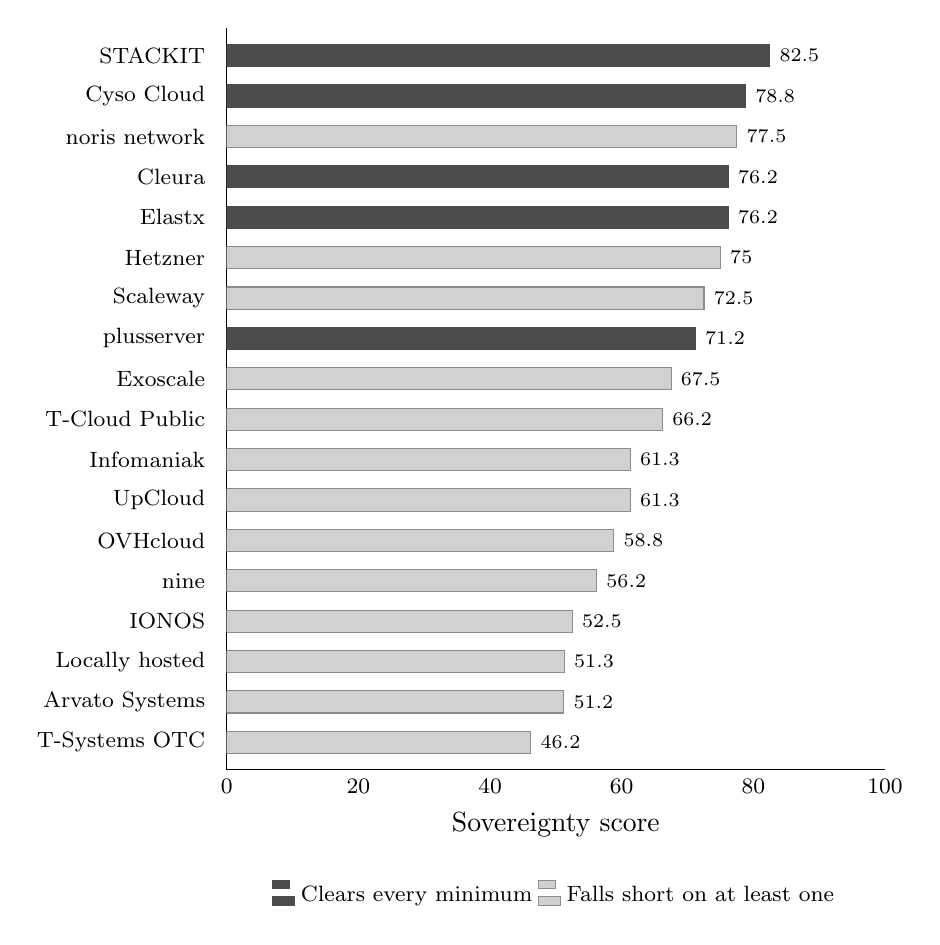
\begin{tikzpicture}
    \begin{axis}[
      xbar,
      width=0.82\textwidth, height=11cm,
      xmin=0, xmax=100,
      xlabel={Sovereignty score},
      bar width=8pt,
      enlarge y limits=0.04,
      symbolic y coords={{T-Systems OTC},{Arvato Systems},{Locally hosted},
                         {IONOS},{nine},{OVHcloud},{UpCloud},{Infomaniak},
                         {T-Cloud Public},{Exoscale},{plusserver},{Scaleway},
                         {Hetzner},{Elastx},{Cleura},{noris network},
                         {Cyso Cloud},{STACKIT}},
      ytick={{T-Systems OTC},{Arvato Systems},{Locally hosted},{IONOS},
             {nine},{OVHcloud},{UpCloud},{Infomaniak},{T-Cloud Public},
             {Exoscale},{plusserver},{Scaleway},{Hetzner},{Elastx},
             {Cleura},{noris network},{Cyso Cloud},{STACKIT}},
      yticklabel style={font=\footnotesize},
      xticklabel style={font=\footnotesize},
      nodes near coords,
      nodes near coords style={font=\scriptsize, text=black},
      legend style={at={(0.5,-0.14)}, anchor=north, legend columns=2,
                    font=\footnotesize, draw=none},
      tick style={draw=none},
      axis x line*=bottom, axis y line*=left,
    ]
      \addplot[xbar, bar shift=0pt, fill=black!70, draw=black!70]
        coordinates {(71.2,{plusserver}) (76.2,{Elastx}) (76.2,{Cleura})
                     (78.8,{Cyso Cloud}) (82.5,{STACKIT})};
      \addplot[xbar, bar shift=0pt, fill=black!18, draw=black!45]
        coordinates {(46.2,{T-Systems OTC}) (51.2,{Arvato Systems})
                     (51.3,{Locally hosted}) (52.5,{IONOS}) (56.2,{nine})
                     (58.8,{OVHcloud}) (61.3,{UpCloud}) (61.3,{Infomaniak})
                     (66.2,{T-Cloud Public}) (67.5,{Exoscale})
                     (72.5,{Scaleway}) (75.0,{Hetzner}) (77.5,{noris network})};
      \legend{Clears every minimum, Falls short on at least one}
    \end{axis}
  \end{tikzpicture}
  \caption{Sovereignty scores for the eighteen providers, with those clearing
           every minimum shown in dark.}
  \label{fig:sov-ranking}
\end{figure}

The dark bars are not the top five. Five providers clear every minimum, but three
that score higher than one of them do not: noris network reaches 77.5 and fails
on supply chain, while plusserver passes on 71.2. Ranking by score alone would
place noris network third and plusserver eighth, and would put forward a provider
that does not meet the requirements.

The two Deutsche Telekom entries also separate sharply. T-Cloud Public scores
66.2 against 46.2 for Open Telekom Cloud --- twenty points between two names for
what the company describes as one platform. That difference is examined in
\cref{sec:study1}.


\section{Study 2 --- Capability Gap Analysis}
\label{sec:method-study2}

This study measures how much of the enterprise's current platform a European
provider could replace. It works from a fixed list of sixty \acs{AWS} services
and asks of every provider whether it offers an equivalent, so what follows
describes where that list came from and how the answers were scored.

The instrument has two parts: a catalogue of services grouped into eleven
categories, and two further dimensions assessed directly rather than from the
catalogue.

\subsection*{The reference catalogue}

The list is drawn from the \acs{AWS} product catalogue
\cite{AWS_Products}, narrowed to what the enterprise uses. Fifty of the sixty
services come from a checklist completed by Alps Alpine
\cite{AlpsAlpine_Checklist}, which asked, for each capability, whether it
was necessary previously, now or later, and named the \acs{AWS} service that
provides it. Fifty-eight lines were marked as needed; several name the same
product, leaving fifty distinct services. A further ten in common use elsewhere
were added, so that a provider is not credited with completeness merely because
the enterprise does not currently need a category.

\todo{The sources for the ten added services.}

The checklist was completed against the platform shown in
\cref{fig:alps-infrastructure} in \cref{app:checklist}, which maps the services the department runs, is
investigating, or expects to need. It is arranged in six stages, from the
networking and identity foundation on the left through to the applications users
see on the right, and it shows why the catalogue is weighted as it is: security
and identity carry the largest number of distinct services, and the specialised
categories --- machine learning and device management --- sit furthest from the
foundation.

\acs{AWS} is the baseline. Every one of the sixty services is its own, so it
scores full marks on every dimension by construction, and each European provider
is measured by how much of the catalogue it matches. The consequence noted in
\cref{sec:research-design} follows from this: a provider offering something
\acs{AWS} does not offer earns nothing for it.

\subsection*{The thirteen dimensions}

The eleven categories are scored from the services they contain. Two further
dimensions --- scalability and performance --- cannot be settled by counting
services, and were assessed instead from what each provider publishes about its
regions, its scaling, its largest instances, its service-level commitments and
its certifications. \Cref{tab:readiness-dimensions} lists all thirteen.

\begin{table}[htbp]
  \centering
  \caption{The thirteen readiness dimensions. Eleven are scored from the
           services they contain; scalability and performance are assessed from
           published documentation.}
  \label{tab:readiness-dimensions}
  \small
  \begin{tabularx}{\textwidth}{@{}l r X@{}}
    \toprule
    \textbf{Dimension} & \textbf{Services} & \textbf{What it covers} \\
    \midrule
    Scalability  & --- & Regions and zones, auto-scaling, largest instance available \\
    Performance  & --- & Published service-level commitments, certifications, storage and network specification \\
    \midrule
    Web and App Hosting &  1 & Managed web and application hosting \\
    Compute      &  6 & Virtual machines, containers, serverless functions, batch \\
    Storage      &  5 & Object, block, archival, backup and shared file storage \\
    Database     &  7 & Relational, document, key-value, time-series, cache, warehouse \\
    Networking   &  7 & Load balancing, private networking, \acs{DNS}, \acs{API} gateway, \acs{CDN}, dedicated links \\
    AI/ML        &  6 & Image recognition, model training, language models, \acs{ETL}, analytics \\
    Security     & 12 & Identity, keys, secrets, certificates, threat detection, firewall, audit logging \\
    Monitoring   &  4 & Metrics, logs, alerting, incident management, cost reporting \\
    Dev/Deploy   &  5 & Build, deployment, pipelines, container registry, infrastructure as code \\
    IoT          &  2 & Device connectivity and fleet management \\
    Messaging    &  5 & Queues, event bus, workflow orchestration, email, streaming \\
    \midrule
    & \textbf{60} & \\
    \bottomrule
  \end{tabularx}
\end{table}

The categories are of very unequal size, which matters when reading a dimension
score. Web and app hosting contains one service, so a provider either scores nothing
there or scores full marks; security contains twelve, so a single service moves
it by four points. The dimensions are therefore comparable as proportions of what
each contains, not as equally fine measurements.

\subsection*{The sixty services}

\Cref{tab:readiness-services} gives the catalogue, grouped by dimension. Services
shown without a mark are those Alps Alpine Europe uses or expects to need; the
ten marked with a dagger are widely used elsewhere and were added so that a
provider is not credited with completeness merely because the department does not
currently need a category.

\begin{table}[htbp]
\centering
\caption{The sixty reference services, by dimension. Unmarked services are used
  by Alps Alpine Europe \cite{AlpsAlpine_Checklist};
  \quad{\normalfont($^{\dagger}$ = popular elsewhere in the industry, added for
  completeness)}}
\label{tab:readiness-services}
\resizebox{\linewidth}{!}{%
\renewcommand{\arraystretch}{1.15}
\begin{tabularx}{1.62\linewidth}{XXXXXXX}
\toprule
\textbf{Scalability}        & \textbf{Performance}       & \textbf{Web and App Hosting (1)} &
\textbf{Compute (6)}        & \textbf{Storage (5)}       & \textbf{Database (7)}    &
\textbf{Networking (7)} \\
\midrule
\textit{Assessed}           & \textit{Assessed}          & Amplify                  &
Lambda                      & S3                         & RDS                      &
App.\ Load Balancer \\
\textit{directly}           & \textit{directly}          &                          &
ECS                         & S3 Glacier                 & DocumentDB               &
Net.\ Load Balancer \\
                            &                            &                          &
EKS                         & EBS                        & DynamoDB                 &
VPC \\
                            &                            &                          &
EC2                         & Backup                     & Timestream               &
Route~53 \\
                            &                            &                          &
Batch                       & EFS$^{\dagger}$            & Aurora$^{\dagger}$       &
API Gateway \\
                            &                            &                          &
Elastic Beanstalk$^{\dagger}$ &                          & ElastiCache$^{\dagger}$  &
CloudFront$^{\dagger}$ \\
                            &                            &                          &
                            &                            & Redshift$^{\dagger}$     &
Direct Connect$^{\dagger}$ \\
\midrule
\textbf{AI/ML (6)}          & \textbf{Security (12)}     & \textbf{Monitoring (4)}  &
\textbf{Dev/Deploy (5)}     & \textbf{IoT (2)}           & \textbf{Messaging (5)}   &
\\
\midrule
Rekognition                 & IAM                        & CloudWatch               &
CodeBuild                   & IoT Core                   & SQS                      & \\
SageMaker                   & Cognito                    & SNS                      &
CodeDeploy                  & IoT Device Mgmt.           & EventBridge              & \\
Bedrock                     & IAM Identity Center        & Systems Manager          &
CodePipeline                &                            & Step Functions           & \\
Glue                        & KMS                        & Cost Explorer            &
ECR                         &                            & SES                      & \\
EMR                         & Secrets Manager            &                          &
CloudFormation$^{\dagger}$  &                            & Kinesis$^{\dagger}$      & \\
Athena                      & Certificate Manager        &                          &
                            &                            &                          & \\
                            & GuardDuty                  &                          &
                            &                            &                          & \\
                            & Security Hub               &                          &
                            &                            &                          & \\
                            & Config                     &                          &
                            &                            &                          & \\
                            & Shield                     &                          &
                            &                            &                          & \\
                            & WAF                        &                          &
                            &                            &                          & \\
                            & CloudTrail$^{\dagger}$     &                          &
                            &                            &                          & \\
\bottomrule
\end{tabularx}
}
\end{table}

\subsection*{The verdicts}

Each service takes one of three verdicts, answered from the provider's published
service documentation:

\begin{itemize}
  \item \textbf{Full (Y)} --- a managed equivalent exists, generally available,
        with comparable function. Two points.
  \item \textbf{Partial (P)} --- an equivalent exists but is in beta,
        feature-limited, or requires a workaround. One point.
  \item \textbf{None (N)} --- no managed equivalent; the capability has to be
        built and run on the provider's raw infrastructure. No points.
\end{itemize}

A verdict of none does not mean the work cannot be done. It means the provider
does not do it for the customer, so the customer does it instead. The gap this
study measures is therefore a transfer of work rather than a hard obstacle, which
is why it is reported separately from the sovereignty result and not merged with
it.

\subsection*{From verdicts to a score}

A dimension score is the points earned across its services as a share of the
points available. Writing $S_c$ for the services in category $c$ and $v_p(s)$ for
the points provider $p$ earned on service $s$:

\begin{equation}
  \label{eq:readiness-dimension}
  d_{p,c} = \frac{\displaystyle\sum_{s \in S_c} v_p(s)}{2\,\lvert S_c \rvert}
            \times 100
\end{equation}

Scalability and performance are not computed this way; each is assigned directly
on the same scale of 0 to 100, against \acs{AWS} at 100.

A provider's overall coverage is the mean of all thirteen dimensions, and its gap
is what remains to the baseline. Since \acs{AWS} scores 100 everywhere, the two
are complements:

\begin{equation}
  \label{eq:readiness-coverage}
  C_p = \frac{1}{13}\sum_{d \in D} d_{p,d}
  \qquad\qquad
  G_p = 100 - C_p
\end{equation}

Worked through: storage contains five services, so ten points are available.
STACKIT offers object storage, block storage and managed backup in full, a cold
storage tier that is less capable than the \acs{AWS} equivalent, and no shared
file system --- six points for the three full, one for the partial, none for the
last, giving seven of ten and a storage score of 70.

\subsection*{What the method produces}

\Cref{tab:readiness-matrix} gives the score on every dimension for the seventeen
providers, with the two Deutsche Telekom platforms treated as one, as explained
in \cref{sec:provider-selection}. The final row is the mean across the providers
for that dimension.

\begin{table}[htbp]
  \centering
  \caption{Coverage by dimension, as a percentage of the \acs{AWS} baseline,
           ranked by mean coverage.}
  \label{tab:readiness-matrix}
  \scriptsize
  \renewcommand{\arraystretch}{1.25}
  \setlength{\tabcolsep}{3.2pt}
  \begin{tabular*}{\textwidth}{@{\extracolsep{\fill}}l *{13}{c} r r@{}}
    \toprule
    \textbf{Provider}
    & \textbf{Scal} & \textbf{Perf} & \textbf{Web} & \textbf{Comp}
    & \textbf{Stor} & \textbf{Data} & \textbf{Netw} & \textbf{AI}
    & \textbf{Sec} & \textbf{Mon} & \textbf{Dev} & \textbf{IoT}
    & \textbf{Msg} & \textbf{Mean} & \textbf{Gap} \\
    \midrule
    T-Systems      & 74 & 87 & 50 & 75 & 90 & 43 & 93 & 50 & 67 & 88 & 70 & 100 & 50 & 72 & 28 \\
    OVHcloud       & 68 & 83 & 50 & 67 & 90 & 43 & 93 & 17 & 62 & 62 & 30 & 25 & 40 & 56 & 44 \\
    STACKIT        & 32 & 80 &  0 & 67 & 70 & 36 & 79 &  8 & 79 & 62 & 30 &  0 & 30 & 44 & 56 \\
    Scaleway       & 42 & 75 &  0 & 83 & 60 & 29 & 50 &  8 & 42 & 50 & 20 & 25 & 40 & 40 & 60 \\
    Exoscale       & 42 & 80 &  0 & 33 & 50 & 29 & 57 &  0 & 21 & 38 &  0 &  0 & 20 & 28 & 72 \\
    plusserver     & 35 & 80 &  0 & 33 & 50 & 21 & 57 &  0 & 29 & 38 & 20 &  0 &  0 & 28 & 72 \\
    UpCloud        & 48 & 83 &  0 & 33 & 60 & 29 & 50 &  0 & 21 & 38 &  0 &  0 &  0 & 28 & 72 \\
    IONOS          & 45 & 78 &  0 & 33 & 50 & 14 & 50 &  0 & 21 & 38 & 20 &  0 &  0 & 27 & 73 \\
    Cleura         & 40 & 77 &  0 & 25 & 50 &  7 & 50 &  0 & 21 & 38 & 10 &  0 & 10 & 25 & 75 \\
    Infomaniak     & 35 & 78 &  0 & 33 & 50 & 14 & 43 &  0 & 25 & 38 & 10 &  0 &  0 & 25 & 75 \\
    Elastx         & 32 & 78 &  0 & 33 & 50 &  7 & 36 &  0 & 21 & 38 & 10 &  0 &  0 & 23 & 77 \\
    Hetzner        & 35 & 72 &  0 & 33 & 50 &  0 & 50 &  0 & 25 & 38 &  0 &  0 &  0 & 23 & 77 \\
    Arvato Systems & 28 & 80 &  0 & 25 & 60 &  7 & 43 &  0 & 17 & 38 &  0 &  0 &  0 & 23 & 77 \\
    Cyso Cloud     & 28 & 75 &  0 & 25 & 50 &  7 & 36 &  0 & 21 & 38 & 10 &  0 &  0 & 22 & 78 \\
    nine           & 25 & 78 &  0 & 25 & 50 &  7 & 36 &  0 & 21 & 38 & 10 &  0 &  0 & 22 & 78 \\
    noris network  & 22 & 82 &  0 & 25 & 50 &  7 & 50 &  0 & 12 & 38 &  0 &  0 &  0 & 22 & 78 \\
    Locally hosted & 15 & 65 &  0 &  8 & 20 &  0 &  7 &  0 &  0 &  0 &  0 &  0 &  0 &  9 & 91 \\
    \midrule
    \textit{mean}  & 38 & 78 &  6 & 39 & 56 & 18 & 52 &  5 & 30 & 42 & 14 &  9 & 11 & & \\
    \bottomrule
  \end{tabular*}
\end{table}

The final row is the more revealing part of the table. Performance is the one
dimension on which European providers are close to the baseline, averaging 78,
and it is also the dimension that separates them least --- every provider falls
between 65 and 87. Storage and networking follow at 56 and 52. At the other end,
the average on \acs{AI} and machine learning is 5 and on web and app hosting 6:
these are not weak areas but largely absent ones.

Six of the sixty services have no equivalent at any provider in the set:
managed application deployment, the key-value store, the time-series database,
the high-performance relational database, the language-model service and workflow
orchestration. Nothing in the assessment can distinguish providers on these,
because none of them offers anything.

\Cref{fig:readiness-profile} draws the four highest-scoring providers against the
\acs{AWS} ceiling, dimension by dimension.

\begin{figure}[htbp]
  \centering
  \begin{tikzpicture}
    \begin{axis}[
      width=\textwidth, height=7.6cm,
      ymin=0, ymax=105,
      ylabel={Coverage of baseline (\%)},
      ylabel style={font=\footnotesize},
      symbolic x coords={Scal,Perf,App,Comp,Stor,Data,Netw,AI,Sec,Mon,Dev,IoT,Msg},
      xtick=data,
      xticklabels={Scal,Perf,Web,Comp,Stor,Data,Netw,AI,Sec,Mon,Dev,IoT,Msg},
      x tick label style={rotate=45, anchor=east, font=\footnotesize},
      yticklabel style={font=\footnotesize},
      ytick={0,20,40,60,80,100},
      grid=major, grid style={black!12},
      legend style={at={(0.5,-0.30)}, anchor=north, legend columns=4,
                    font=\footnotesize, draw=none},
      tick style={draw=none},
      axis x line*=bottom, axis y line*=left,
    ]
      \addplot[cBase, dashed, very thick, mark=none] coordinates {
        (Scal,100) (Perf,100) (App,100) (Comp,100) (Stor,100) (Data,100)
        (Netw,100) (AI,100) (Sec,100) (Mon,100) (Dev,100) (IoT,100) (Msg,100)};
      \addplot[cProvA, thick, mark=*, mark size=1.8pt] coordinates {
        (Scal,74) (Perf,87) (App,50) (Comp,75) (Stor,90) (Data,43)
        (Netw,93) (AI,50) (Sec,67) (Mon,88) (Dev,70) (IoT,100) (Msg,50)};
      \addplot[cProvB, thick, mark=square*, mark size=1.6pt] coordinates {
        (Scal,68) (Perf,83) (App,50) (Comp,67) (Stor,90) (Data,43)
        (Netw,93) (AI,17) (Sec,62) (Mon,62) (Dev,30) (IoT,25) (Msg,40)};
      \addplot[cProvC, thick, mark=triangle*, mark size=2.1pt] coordinates {
        (Scal,32) (Perf,80) (App,0) (Comp,67) (Stor,70) (Data,36)
        (Netw,79) (AI,8) (Sec,79) (Mon,62) (Dev,30) (IoT,0) (Msg,30)};
      \legend{\acs{AWS} baseline, T-Systems, OVHcloud, STACKIT}
    \end{axis}
  \end{tikzpicture}
  \caption{Coverage by dimension for the three leading providers against the
           \acs{AWS} baseline.}
  \label{fig:readiness-profile}
\end{figure}

The same three are shown as coverage profiles in \cref{fig:readiness-radar},
where the area enclosed by each shape is the share of the catalogue it reaches.
The shapes are not merely smaller than the baseline; they are indented in
different places, which is what makes the providers hard to rank on a single
figure.

\begin{figure}[htbp]
  \centering
  \begin{tikzpicture}
    \begin{polaraxis}[
      scale only axis,
      width=8.4cm, height=8.4cm,
      ymin=0, ymax=100,
      xtick={0,27.692,55.385,83.077,110.769,138.462,166.154,193.846,
             221.538,249.231,276.923,304.615,332.308},
      xticklabels={Scal,Perf,Web,Comp,Stor,Data,Netw,AI,Sec,Mon,Dev,IoT,Msg},
      xticklabel style={font=\scriptsize},
      ytick={20,40,60,80,100},
      yticklabel style={font=\tiny, black!55},
      grid=both, grid style={black!15},
      legend style={at={(0.5,-0.06)}, anchor=north, legend columns=4,
                    font=\footnotesize, draw=none},
    ]
      \addplot[cBase, dashed, very thick, mark=none] coordinates {
        (0,100) (27.692,100) (55.385,100) (83.077,100) (110.769,100)
        (138.462,100) (166.154,100) (193.846,100) (221.538,100)
        (249.231,100) (276.923,100) (304.615,100) (332.308,100) (360,100)};
      \addplot[cProvA, thick, mark=*, mark size=1.5pt,
               fill=cProvA, fill opacity=0.12] coordinates {
        (0,74) (27.692,87) (55.385,50) (83.077,75) (110.769,90)
        (138.462,43) (166.154,93) (193.846,50) (221.538,67)
        (249.231,88) (276.923,70) (304.615,100) (332.308,50) (360,74)};
      \addplot[cProvB, thick, mark=square*, mark size=1.4pt,
               fill=cProvB, fill opacity=0.12] coordinates {
        (0,68) (27.692,83) (55.385,50) (83.077,67) (110.769,90)
        (138.462,43) (166.154,93) (193.846,17) (221.538,62)
        (249.231,62) (276.923,30) (304.615,25) (332.308,40) (360,68)};
      \addplot[cProvC, thick, mark=triangle*, mark size=1.8pt,
               fill=cProvC, fill opacity=0.12] coordinates {
        (0,32) (27.692,80) (55.385,0) (83.077,67) (110.769,70)
        (138.462,36) (166.154,79) (193.846,8) (221.538,79)
        (249.231,62) (276.923,30) (304.615,0) (332.308,30) (360,32)};
      \legend{\acs{AWS} baseline, T-Systems, OVHcloud, STACKIT}
    \end{polaraxis}
  \end{tikzpicture}
  \caption{Coverage profiles of the three leading providers against the
           \acs{AWS} baseline, across the thirteen dimensions.}
  \label{fig:readiness-radar}
\end{figure}

\Cref{fig:readiness-verdicts} shows what lies behind the dimension scores: how
many of the sixty services each provider covers fully, partly, or not at all.

\begin{figure}[htbp]
  \centering
  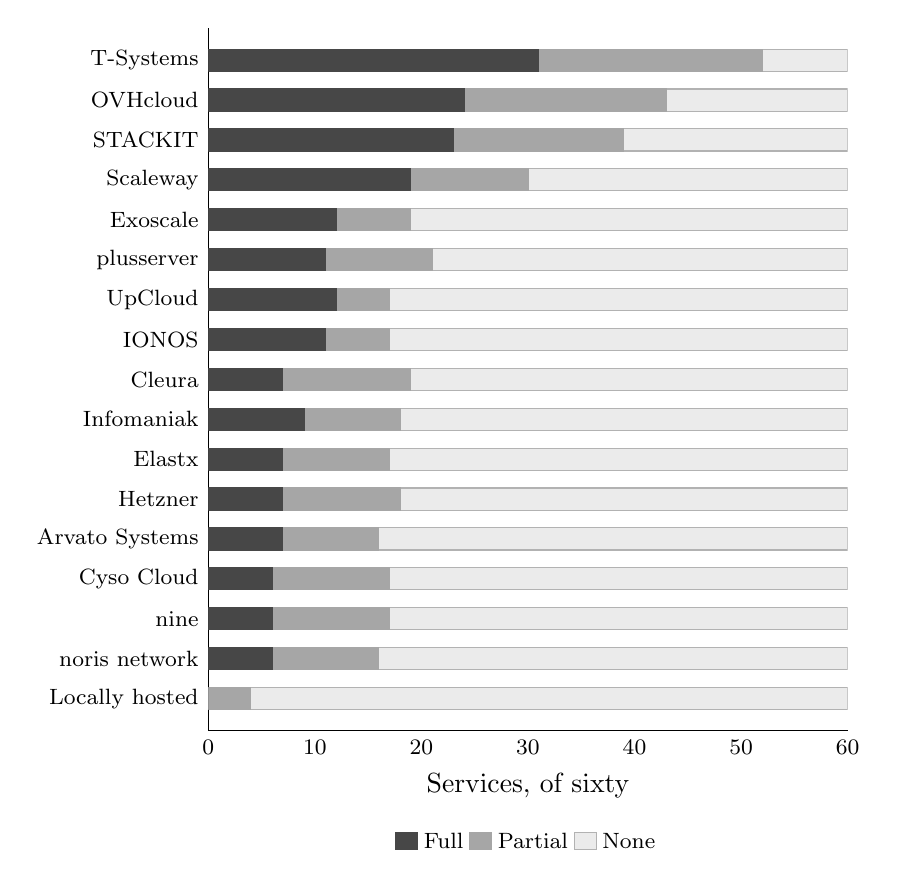
\begin{tikzpicture}
    \begin{axis}[
      xbar stacked,
      width=0.80\textwidth, height=10.5cm,
      xmin=0, xmax=60,
      xlabel={Services, of sixty},
      bar width=8pt,
      enlarge y limits=0.05,
      symbolic y coords={{Locally hosted},{noris network},{nine},{Cyso Cloud},
                         {Arvato Systems},{Hetzner},{Elastx},{Infomaniak},
                         {Cleura},{IONOS},{UpCloud},{plusserver},{Exoscale},
                         {Scaleway},{STACKIT},{OVHcloud},{T-Systems}},
      ytick={{Locally hosted},{noris network},{nine},{Cyso Cloud},
             {Arvato Systems},{Hetzner},{Elastx},{Infomaniak},{Cleura},
             {IONOS},{UpCloud},{plusserver},{Exoscale},{Scaleway},
             {STACKIT},{OVHcloud},{T-Systems}},
      yticklabel style={font=\footnotesize},
      xticklabel style={font=\footnotesize},
      legend style={at={(0.5,-0.13)}, anchor=north, legend columns=3,
                    font=\footnotesize, draw=none},
      tick style={draw=none},
      axis x line*=bottom, axis y line*=left,
    ]
      \addplot[fill=black!72, draw=black!72] coordinates {
        (0,{Locally hosted}) (6,{noris network}) (6,{nine}) (6,{Cyso Cloud})
        (7,{Arvato Systems}) (7,{Hetzner}) (7,{Elastx}) (9,{Infomaniak})
        (7,{Cleura}) (11,{IONOS}) (12,{UpCloud}) (11,{plusserver})
        (12,{Exoscale}) (19,{Scaleway}) (23,{STACKIT}) (24,{OVHcloud})
        (31,{T-Systems})};
      \addplot[fill=black!35, draw=black!35] coordinates {
        (4,{Locally hosted}) (10,{noris network}) (11,{nine}) (11,{Cyso Cloud})
        (9,{Arvato Systems}) (11,{Hetzner}) (10,{Elastx}) (9,{Infomaniak})
        (12,{Cleura}) (6,{IONOS}) (5,{UpCloud}) (10,{plusserver})
        (7,{Exoscale}) (11,{Scaleway}) (16,{STACKIT}) (19,{OVHcloud})
        (21,{T-Systems})};
      \addplot[fill=black!8, draw=black!30] coordinates {
        (56,{Locally hosted}) (44,{noris network}) (43,{nine}) (43,{Cyso Cloud})
        (44,{Arvato Systems}) (42,{Hetzner}) (43,{Elastx}) (42,{Infomaniak})
        (41,{Cleura}) (43,{IONOS}) (43,{UpCloud}) (39,{plusserver})
        (41,{Exoscale}) (30,{Scaleway}) (21,{STACKIT}) (17,{OVHcloud})
        (8,{T-Systems})};
      \legend{Full, Partial, None}
    \end{axis}
  \end{tikzpicture}
  \caption{Verdicts across the sixty reference services, ordered by mean
           coverage.}
  \label{fig:readiness-verdicts}
\end{figure}

The figure separates two groups. Four providers --- T-Systems, OVHcloud, STACKIT
and Scaleway --- cover between a third and a half of the catalogue outright. The
remaining twelve cluster tightly: six to twelve services in full, most of the
rest missing. Locally hosted infrastructure marks the floor, with no managed
equivalent to anything and four partials.

Behind those totals is a service-by-service picture.
\Cref{tab:readiness-services-compare} sets the four leading providers against
the baseline one service at a time, and gives for each service how many of the
seventeen offer a full equivalent.

\footnotesize
\begin{longtable}{@{}p{4.9cm} *{4}{>{\centering\arraybackslash}p{1.75cm}} r@{}}
  \caption{Service-by-service comparison against the \acs{AWS} baseline for
           the four leading providers. Y = a managed equivalent exists in
           full, P = partial, -- = none. The last column counts how many of
           the seventeen offer a full equivalent.}
  \label{tab:readiness-services-compare}\\
  \toprule
  \textbf{\acs{AWS} service} & \textbf{T-Systems} & \textbf{OVHcloud} & \textbf{STACKIT} & \textbf{Scaleway} & \textbf{Full/17} \\
  \midrule
  \endfirsthead
  \toprule
  \textbf{\acs{AWS} service} & \textbf{T-Systems} & \textbf{OVHcloud} & \textbf{STACKIT} & \textbf{Scaleway} & \textbf{Full/17} \\
  \midrule
  \endhead
  \bottomrule
  \endfoot
  \multicolumn{6}{@{}l}{\textit{Web and App Hosting}}\\
  Amplify & P & P & -- & -- & 0 \\
  \midrule
  \multicolumn{6}{@{}l}{\textit{Compute}}\\
  Lambda & Y & P & P & Y & 2 \\
  ECS & Y & Y & Y & Y & 4 \\
  EKS & Y & Y & Y & Y & 10 \\
  EC2 & Y & Y & Y & Y & 16 \\
  Batch & P & P & P & Y & 1 \\
  Elastic Beanstalk & -- & -- & -- & -- & 0 \\
  \midrule
  \multicolumn{6}{@{}l}{\textit{Storage}}\\
  S3 & Y & Y & Y & Y & 16 \\
  S3 Glacier & P & Y & P & P & 1 \\
  EBS & Y & Y & Y & Y & 16 \\
  Backup & Y & Y & Y & P & 5 \\
  EFS & Y & P & -- & -- & 1 \\
  \midrule
  \multicolumn{6}{@{}l}{\textit{Database}}\\
  RDS & Y & Y & Y & Y & 9 \\
  DocumentDB & P & P & -- & P & 0 \\
  DynamoDB & -- & -- & -- & -- & 0 \\
  Timestream & -- & -- & -- & -- & 0 \\
  Aurora & -- & -- & -- & -- & 0 \\
  ElastiCache & Y & Y & Y & P & 5 \\
  Redshift & P & P & P & -- & 0 \\
  \midrule
  \multicolumn{6}{@{}l}{\textit{Networking}}\\
  Application Load Balancer & Y & Y & Y & Y & 9 \\
  Network Load Balancer & Y & Y & Y & P & 4 \\
  VPC & Y & Y & Y & Y & 16 \\
  Route 53 & Y & Y & Y & Y & 10 \\
  API Gateway & Y & P & P & -- & 1 \\
  CloudFront & P & Y & -- & -- & 1 \\
  Direct Connect & Y & Y & Y & -- & 5 \\
  \midrule
  \multicolumn{6}{@{}l}{\textit{AI/ML}}\\
  Rekognition & P & -- & -- & -- & 0 \\
  SageMaker & Y & P & P & P & 1 \\
  Bedrock & -- & -- & -- & -- & 0 \\
  Glue & P & -- & -- & -- & 0 \\
  EMR & P & P & -- & -- & 0 \\
  Athena & P & -- & -- & -- & 0 \\
  \midrule
  \multicolumn{6}{@{}l}{\textit{Security}}\\
  IAM & Y & Y & Y & Y & 14 \\
  Cognito & -- & P & P & -- & 0 \\
  IAM Identity Center & -- & P & P & -- & 0 \\
  KMS & Y & Y & Y & Y & 4 \\
  Secrets Manager & P & P & Y & Y & 2 \\
  Certificate Manager & Y & Y & Y & Y & 4 \\
  GuardDuty & P & P & P & -- & 0 \\
  Security Hub & P & -- & P & -- & 0 \\
  Config & P & -- & P & -- & 0 \\
  Shield & Y & Y & Y & P & 3 \\
  WAF & Y & Y & Y & -- & 3 \\
  CloudTrail & Y & P & Y & P & 2 \\
  \midrule
  \multicolumn{6}{@{}l}{\textit{Monitoring}}\\
  CloudWatch & Y & P & P & P & 1 \\
  SNS & Y & P & P & P & 1 \\
  Systems Manager & P & P & P & -- & 0 \\
  Cost Explorer & Y & Y & Y & Y & 16 \\
  \midrule
  \multicolumn{6}{@{}l}{\textit{Dev/Deploy}}\\
  CodeBuild & P & -- & -- & -- & 0 \\
  CodeDeploy & P & -- & -- & -- & 0 \\
  CodePipeline & P & -- & -- & -- & 0 \\
  ECR & Y & Y & Y & Y & 6 \\
  CloudFormation & Y & P & P & -- & 1 \\
  \midrule
  \multicolumn{6}{@{}l}{\textit{IoT}}\\
  IoT Core & Y & P & -- & P & 1 \\
  IoT Device Management & Y & -- & -- & -- & 1 \\
  \midrule
  \multicolumn{6}{@{}l}{\textit{Messaging}}\\
  SQS & Y & Y & Y & Y & 4 \\
  EventBridge & P & -- & -- & -- & 0 \\
  Step Functions & -- & -- & -- & -- & 0 \\
  SES & P & Y & P & Y & 2 \\
  Kinesis & P & -- & -- & -- & 0 \\
\end{longtable}
\normalsize

\Cref{fig:readiness-ranking} ranks the providers by mean coverage, with the
remaining gap to the baseline shown alongside.

\begin{figure}[htbp]
  \centering
  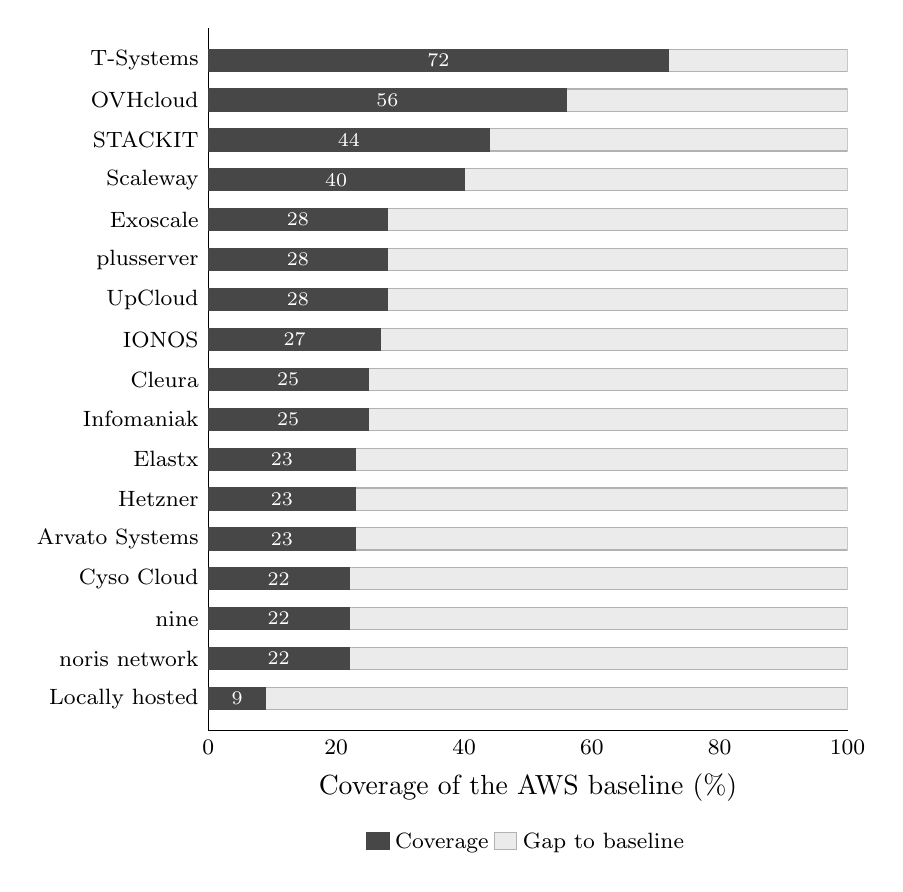
\begin{tikzpicture}
    \begin{axis}[
      xbar stacked,
      width=0.80\textwidth, height=10.5cm,
      xmin=0, xmax=100,
      xlabel={Coverage of the \acs{AWS} baseline (\%)},
      bar width=8pt,
      enlarge y limits=0.05,
      symbolic y coords={{Locally hosted},{noris network},{nine},{Cyso Cloud},
                         {Arvato Systems},{Hetzner},{Elastx},{Infomaniak},
                         {Cleura},{IONOS},{UpCloud},{plusserver},{Exoscale},
                         {Scaleway},{STACKIT},{OVHcloud},{T-Systems}},
      ytick={{Locally hosted},{noris network},{nine},{Cyso Cloud},
             {Arvato Systems},{Hetzner},{Elastx},{Infomaniak},{Cleura},
             {IONOS},{UpCloud},{plusserver},{Exoscale},{Scaleway},
             {STACKIT},{OVHcloud},{T-Systems}},
      yticklabel style={font=\footnotesize},
      xticklabel style={font=\footnotesize},
      legend style={at={(0.5,-0.13)}, anchor=north, legend columns=2,
                    font=\footnotesize, draw=none},
      tick style={draw=none},
      axis x line*=bottom, axis y line*=left,
    ]
      \addplot[fill=black!72, draw=black!72,
               nodes near coords,
               nodes near coords style={font=\scriptsize, text=white}]
        coordinates {
        (9,{Locally hosted}) (22,{noris network}) (22,{nine}) (22,{Cyso Cloud})
        (23,{Arvato Systems}) (23,{Hetzner}) (23,{Elastx}) (25,{Infomaniak})
        (25,{Cleura}) (27,{IONOS}) (28,{UpCloud}) (28,{plusserver})
        (28,{Exoscale}) (40,{Scaleway}) (44,{STACKIT}) (56,{OVHcloud})
        (72,{T-Systems})};
      \addplot[fill=black!8, draw=black!30] coordinates {
        (91,{Locally hosted}) (78,{noris network}) (78,{nine}) (78,{Cyso Cloud})
        (77,{Arvato Systems}) (77,{Hetzner}) (77,{Elastx}) (75,{Infomaniak})
        (75,{Cleura}) (73,{IONOS}) (72,{UpCloud}) (72,{plusserver})
        (72,{Exoscale}) (60,{Scaleway}) (56,{STACKIT}) (44,{OVHcloud})
        (28,{T-Systems})};
      \legend{Coverage, Gap to baseline}
    \end{axis}
  \end{tikzpicture}
  \caption{Mean coverage across the thirteen dimensions, with the remaining gap
           to the \acs{AWS} baseline.}
  \label{fig:readiness-ranking}
\end{figure}

This ranking runs close to the opposite of the sovereignty ranking in
\cref{fig:sov-ranking}. T-Systems Open Telekom Cloud scored lowest of the
eighteen on sovereignty and covers most of the catalogue here. STACKIT scored
highest on sovereignty and comes third. noris network was third on sovereignty
and sixteenth here. The two results are measuring different things, and a
provider that does well on one gives no reason to expect it will do well on the
other --- which is why they are kept apart until \cref{ch:evaluation}.


\section{Study 3 --- Financial Viability}
\label{sec:method-study3}

Sovereignty has to be paid for. The first two studies asked whether a provider is
legally able to protect the data it holds and technically able to run the work,
but both of those are things a provider must keep buying. Data centres, servers
and network capacity are not bought once, and a provider that cannot fund them
cannot offer the services counted in \cref{sec:method-study2}, whatever its legal
standing. A provider that runs out of money altogether offers nothing at all.

The economics make this harder for a European entrant than for the incumbent.
The \ac{OECD} finds that establishing a cloud service carries high fixed costs,
and that most of the capital involved --- data centres, network infrastructure,
servers and hardware --- is sunk, in the sense that it cannot be recovered if the
provider withdraws \cite{OECD_CloudCompetition_2025}. Committing to build is
therefore close to irreversible. Scale then compounds the difficulty: because the
largest providers can invest at a level almost no entrant can match, they operate
at lower marginal cost, and the same report concludes that a supplier unwilling
to match those investment levels \enquote{will likely incur higher costs to
deliver the same level of service as the hyperscalers}
\cite{OECD_CloudCompetition_2025}.

That is the position every provider in this study occupies, and it carries a
consequence for sovereignty that the first two studies cannot see. A sovereign
alternative exists in practice only if somebody can afford to build and keep
running it. A provider may hold the strongest legal position in Europe and still
be unable to fund the next data centre, in which case the sovereignty it offers
is available only for the workloads it already supports.

This study therefore examines the money behind each provider, and what it implies
for the years a contract has to run: how fast each is closing the capability gap
against the \acs{AWS} baseline and when it would draw level, what it earns, what
it spends to gain that ground, and where that money comes from. The aim is to
establish how far finance accounts for the progress these providers have made,
and for the distance still left.

Five providers are carried into this study, with \acs{AWS} again as the baseline.
\Cref{tab:study3-providers} gives them, and what the first two studies found
about each.

\begin{table}[htbp]
  \centering
  \caption{The five providers carried into Study~3, with their results from the
           first two studies.}
  \label{tab:study3-providers}
  \small
  \begin{tabularx}{\textwidth}{@{}l l r r X@{}}
    \toprule
    \textbf{Provider} & \textbf{Parent company}
      & \textbf{Sov.} & \textbf{Cap.}
      & \textbf{Reason for inclusion} \\
    \midrule
    \acs{AWS}      & Amazon.com, Inc.      & ---  & 100 & Baseline \\
    \midrule
    T-Cloud Public & Deutsche Telekom \acs{AG} & 66.2 & 72 & Highest capability \\
    OVHcloud       & OVH Groupe            & 58.8 & 56 & Second highest capability \\
    STACKIT        & Schwarz Group         & 82.5 & 44 & Third highest capability \\
    Scaleway       & iliad Group           & 72.5 & 40 & Fourth highest capability \\
    IONOS          & United Internet \acs{AG} & 52.5 & 27 & Finances publicly accessible \\
    \bottomrule
  \end{tabularx}
\end{table}

Four of the five are the highest-ranked on capability in
\cref{sec:method-study2}. IONOS was included because it publishes financial
accounts of its own, which is what this study needs. 

Sovereignty rank played no part in the selection, and the table shows why it
could not have: only STACKIT clears every minimum in \cref{sec:method-study1}.
Carrying forward only the providers that passed would have left a single
candidate and nothing to compare it against. This study aims to evaluate whether
the financial position of the providers is consistent with the sovereignty and
capability they offer. 


\subsection{Closing the gap to AWS}

Will these \acs{EU} cloud providers catch up with hyperscalers like \acs{AWS}?
Two figures are used to answer that: the \textbf{parity speed}, the rate of
growth in capability each provider has achieved since it launched, and the
\textbf{parity year}, the year it would reach the same capability as \acs{AWS} if
that growth continues.

Both rest on a starting year, and the providers do not share one. To establish
it, the development phase of each was examined, as shown in
\cref{fig:launch-dates}, and the external launch date was considered --- the year the platform was made available to the general public, not to internal teams or a free trial.

\begin{figure}[htbp]
  \centering
  % Years are plotted as an offset from 1999: using the year itself as a
  % coordinate multiplies out past TikZ's maximum dimension.
  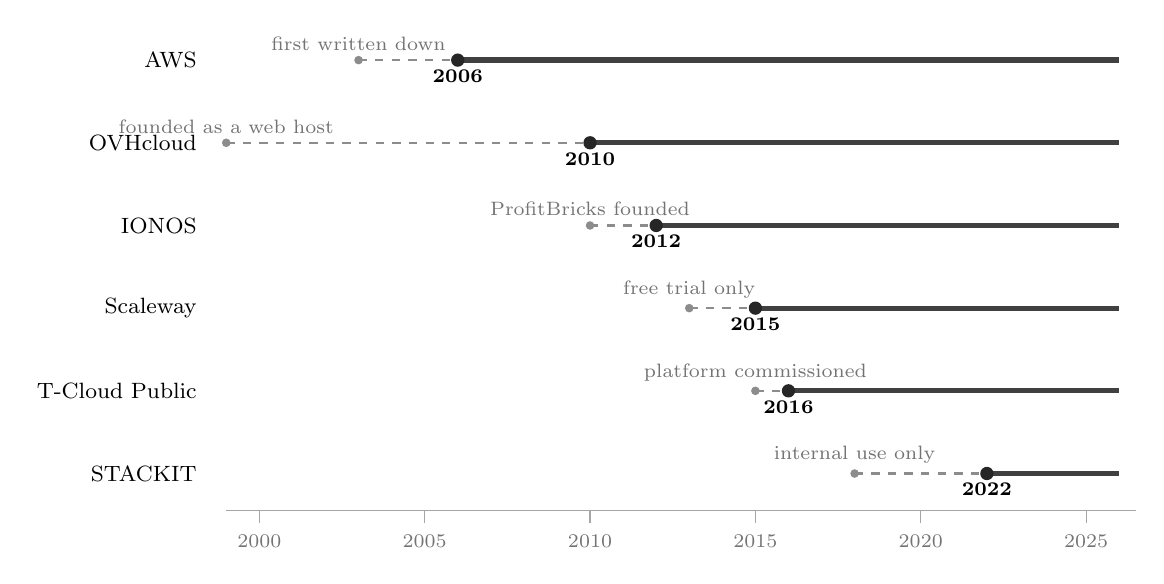
\begin{tikzpicture}[x=0.42cm, y=1.05cm]
    \def\yzero{1999}
    \draw[black!35] (0,-0.45) -- (27.5,-0.45);
    \foreach \yr in {2000,2005,2010,2015,2020,2025} {
      \pgfmathsetmacro\xx{\yr-\yzero}
      \draw[black!35] (\xx,-0.45) -- (\xx,-0.60);
      \node[below, font=\scriptsize, black!55] at (\xx,-0.62) {\yr};
    }
    \foreach \row/\start/\launch/\name/\origin in {%
      5/2003/2006/{\acs{AWS}}/{first written down},
      4/1999/2010/{OVHcloud}/{founded as a web host},
      3/2010/2012/{IONOS}/{ProfitBricks founded},
      2/2013/2015/{Scaleway}/{free trial only},
      1/2015/2016/{T-Cloud Public}/{platform commissioned},
      0/2018/2022/{STACKIT}/{internal use only}}
    {
      \pgfmathsetmacro\xs{\start-\yzero}
      \pgfmathsetmacro\xl{\launch-\yzero}
      \node[left, font=\footnotesize] at (-0.6,\row) {\name};
      \draw[black!45, dashed, line width=0.9pt] (\xs,\row) -- (\xl,\row);
      \node[circle, fill=black!45, inner sep=1.1pt] at (\xs,\row) {};
      \node[above, font=\scriptsize, black!55] at (\xs,\row) {\origin};
      \draw[black!75, line width=1.9pt] (\xl,\row) -- (27,\row);
      \node[circle, fill=black!85, inner sep=1.7pt] at (\xl,\row) {};
      \node[below, font=\scriptsize\bfseries] at (\xl,\row) {\launch};
    }
  \end{tikzpicture}
  \caption{Launch phase of each provider — the time taken from the beginning of development until the service is made publicly available.}
  \label{fig:launch-dates}
\end{figure}

The dashed part is the time spent building before anything could be bought; the solid part is the time
on sale. The external launch year used in the calculation is shown in
bold. 

\begin{itemize}
  \item \textbf{\acs{AWS}} --- the idea was written down inside Amazon in 2003
        and built from 2004 \cite{Black_EC2Origins_2009}. Its storage service
        went on sale in \textbf{2006}, the year used
        \cite{AWS_FirstFiveYears}.
  \item \textbf{OVHcloud} --- founded in 1999, but as a web hosting company. It
        began building its own data centres in 2006 and sold no cloud product
        until \textbf{2010}, the year used \cite{OVHcloud_History}.
  \item \textbf{IONOS} --- the platform is ProfitBricks, founded in Berlin in
        2010 \cite{IONOS_ProfitBricks_2018} and selling by \textbf{2012}, the
        year used: it had around a thousand customers by that November
        \cite{ProfitBricks_DCK_2012}. United Internet bought it in 2017 and the
        business was renamed IONOS in 2018
        \cite{IONOS_ProfitBricks_2018}, so the familiar name is six years
        younger than the platform behind it.
  \item \textbf{Scaleway} --- ran from 2013 as a free trial under the name
        Online Labs. It went on sale as Scaleway in \textbf{2015}, the year
        used \cite{Scaleway_About}.
  \item \textbf{T-Cloud Public} --- the platform was commissioned in 2015 under
        a partnership with Huawei and opened to customers as Open Telekom Cloud
        in \textbf{2016}, the year used \cite{OTC_GoesLive_2016}.
  \item \textbf{STACKIT} --- built in 2018 to run Lidl and Kaufland alone. It
        opened to customers outside the Schwarz group in \textbf{2022}, the year
        used \cite{STACKIT_Launch_2022}.
\end{itemize}

The dashed part is therefore left out in every case, the baseline included.
\acs{AWS} ran three years before it had anything to sell, and STACKIT four;
neither is credited with them.

With a start year fixed, the capability score becomes a rate. The parity speed is
the score divided by the years the provider has been selling, and the parity year
is the point at which that speed would carry it to the baseline of 100. The year
of assessment is 2026 throughout.

\begin{align}
  \label{eq:parity-speed}
  \text{parity speed (points/year)}
    &= \frac{\text{score}}{2026 - \text{launch year}} \\[0.6em]
  \label{eq:parity-year}
  \text{parity year}
    &\approx 2026 + \frac{100 - \text{score}}{\text{parity speed}}
\end{align}

Worked through for T-Cloud Public: it scores 72.1 and has been selling since
2016, so ten years for 72.1 points, a rate of 7.2 points a year. The remaining
27.9 points at that rate take a further four years, giving 2030.

The parity year is an illustration, not a forecast, for three reasons. First, no
provider has undertaken to keep improving at the rate it has managed so far, and
none is obliged to. Second, it assumes progress is even, which it is not: the first
services a provider builds are the ones its customers ask for most, and the
remainder get harder.

Third, it holds the baseline still. \acs{AWS} sits at 100 throughout, but it is not
a fixed target. It adds services continuously, and the catalogue used in
\cref{sec:method-study2} records only what it offered at the time of assessment.
A provider closing on 100 is therefore closing on where \acs{AWS} stood in 2026,
not where it will stand in 2038, for example. Every date that follows is the earliest a
provider could arrive, on the most favourable reading available to it, and the
real distance is wider than the chart can show. Whether it is wider by a few
years or by an unbridgeable margin depends on how fast \acs{AWS} keeps extending
its own catalogue, which this study does not attempt to predict.

The figure is reported because it expresses the gap in years rather than points,
and years are the unit a contract is written in.

\Cref{fig:parity-projection} draws the result. The solid lines are the record so
far, from launch to the year of assessment. The dashed lines carry each rate
forward to the baseline.

\begin{figure}[htbp]
  \centering
  \begin{tikzpicture}
    \begin{axis}[
      width=0.96\textwidth, height=8.2cm,
      xmin=2006, xmax=2066, ymin=0, ymax=108,
      xlabel={Year}, ylabel={Capability score},
      xlabel style={font=\footnotesize}, ylabel style={font=\footnotesize},
      xtick={2006,2016,2026,2036,2046,2056,2066},
      ytick={0,20,40,60,80,100},
      ticklabel style={font=\footnotesize},
      % years are years, not quantities: suppress the thousands separator
      scaled x ticks=false,
      x tick label style={/pgf/number format/1000 sep={}},
      grid=major, grid style={black!10},
      axis on top,
      legend style={at={(0.5,-0.22)}, anchor=north, legend columns=3,
                    font=\footnotesize, draw=none, column sep=1ex},
      tick style={draw=none},
      axis x line*=bottom, axis y line*=left,
      clip=false,
    ]
      % projection zone, everything right of the year of assessment
      \fill[black!4] (axis cs:2026,0) rectangle (axis cs:2066,108);
      % the baseline the providers are measured against
      \addplot[cBase, dashed, very thick, mark=none, forget plot]
        coordinates {(2006,100) (2066,100)};
      \node[anchor=south east, font=\scriptsize, cBase]
        at (axis cs:2066,100) {\acs{AWS} baseline};
      % year of assessment, and the Digital Decade target
      \draw[black!45, dashed] (axis cs:2026,0) -- (axis cs:2026,108);
      \node[anchor=south, font=\scriptsize, black!55, rotate=90]
        at (axis cs:2025.2,2) {assessed 2026};
      \draw[black!45, dashed] (axis cs:2030,0) -- (axis cs:2030,108);
      \node[anchor=south, font=\scriptsize, black!55, rotate=90]
        at (axis cs:2029.2,2) {2030 EC Digital Decade};

      % record so far (solid) and the rate carried forward (dashed)
      \addplot[cProvA, very thick] coordinates {(2016,0) (2026,72.1)};
      \addplot[cProvA, thick, dashed, mark=*, mark size=1.6pt,
               forget plot] coordinates {(2026,72.1) (2029.9,100)};
      \addplot[cProvC, very thick] coordinates {(2022,0) (2026,44.1)};
      \addplot[cProvC, thick, dashed, mark=*, mark size=1.6pt,
               forget plot] coordinates {(2026,44.1) (2031.1,100)};
      \addplot[cProvB, very thick] coordinates {(2010,0) (2026,56.2)};
      \addplot[cProvB, thick, dashed, mark=*, mark size=1.6pt,
               forget plot] coordinates {(2026,56.2) (2038.5,100)};
      \addplot[cProvD, very thick] coordinates {(2015,0) (2026,40.3)};
      \addplot[cProvD, thick, dashed, mark=*, mark size=1.6pt,
               forget plot] coordinates {(2026,40.3) (2042.3,100)};
      \addplot[cProvE, very thick] coordinates {(2012,0) (2026,26.8)};
      \addplot[cProvE, thick, dashed, mark=*, mark size=1.6pt,
               forget plot] coordinates {(2026,26.8) (2064.2,100)};
      \legend{T-Cloud Public, STACKIT, OVHcloud, Scaleway, IONOS}
    \end{axis}
  \end{tikzpicture}
  \caption{Capability added since launch (solid) and the same rate carried
           forward to the \acs{AWS} baseline (dashed). The shaded area is
           projection rather than record.}
  \label{fig:parity-projection}
\end{figure}

The steepest line belongs to the youngest provider. STACKIT has been selling for
four years and has added capability faster than anyone in the set, which is what
places it at the baseline in 2031 despite starting last. T-Cloud Public arrives a
year earlier from a higher score and a gentler slope. Both fall close to the
Union's 2030 target for digital capability, and the remaining three do not:
OVHcloud in 2038, Scaleway in 2042, and IONOS not until the 2060s.

The IONOS figure indicates a direction rather than a date. Thirty-eight years is
past any horizon a procurement decision occupies, and the figure reflects what
IONOS is: a business whose capability score is low because it sells hosting and
domains rather than infrastructure, not because it is building infrastructure
slowly. The projection assumes every provider is running the same race, and that
is the assumption it exposes.

\subsection{Cloud Providers, and their parent company}

The parity speed shows how fast each provider has been adding capability, but not
what that capability cost or who paid for it. Those are the questions the rest of
this study addresses, and it addresses them by assessing each provider together
with the company that owns it rather than on its own.

\Cref{tab:study3-providers} shows why. Every provider sits inside a parent
company, the baseline included --- Amazon reports
\acs{AWS}'s results separately within its own accounts. A provider with an owner
behind it can be funded
through years of losses, can build at a scale its own revenue would never
support, and can be sustained for strategic reasons that have nothing to do with
whether the cloud business itself is profitable.

The parents are not alike, and the difference matters more than the fact of
having one. Deutsche Telekom, Schwarz, iliad and Amazon all run substantial
businesses outside cloud. Deutsche Telekom and iliad are telecommunications
operators; Schwarz and Amazon are retailers. From any of them a cloud arm can
be subsidised indefinitely. OVH Groupe does not:
it is the listed holding company for the cloud business and essentially nothing
else, majority-held by the founding family. When OVHcloud needs capital it goes
to the markets, which is what it did in 2021 \cite{OVHcloud_IPO}. When STACKIT
needs capital it asks Schwarz \cite{SchwarzDigits_Luebbenau_2025}.


The owners also differ in how much they are willing to say, and that turns out to
shape what this study can measure. \Cref{tab:study3-disclosure} sets out what each
one actually publishes.

\begin{table}[htbp]
  \centering
  \caption{What each owner publishes about its cloud business.}
  \label{tab:study3-disclosure}
  \footnotesize
  \begin{tabularx}{\textwidth}{@{}l l X l@{}}
    \toprule
    Provider & Owner & Revenue of the cloud business & Revenue by country \\
    \midrule
    \acs{AWS}      & Amazon           & Published, as one of three reporting segments & Not published \\
    OVHcloud       & OVH Groupe       & Published --- it is the whole company          & Published, three regions \\
    IONOS          & United Internet  & Published separately since 2020                & German and non-German only \\
    T-Cloud Public & Deutsche Telekom & Not published                                  & Published, as percentages \\
    Scaleway       & iliad            & Not published                                  & Published, country by country \\
    STACKIT        & Schwarz Group    & Not published                                  & Not published \\
    \bottomrule
  \end{tabularx}

  \vspace{2pt}
  \footnotesize
  Sources. \cite{Amazon_10K_2025,OVHcloud_URD_2025,IONOS_AR_2025,UnitedInternet_AR_2025,%
  DT_AR_2025,Iliad_AFR_2025,Schwarz_Figures_FY2025}.
\end{table}

The pattern follows how each owner is held. Amazon, OVH Groupe, United Internet
and IONOS are listed and publish the most. Deutsche Telekom is listed and iliad
was until 2021, and both publish where their revenue is earned but not what their
cloud business takes in. The Schwarz Group is privately held, answers to no
stock-market regulator on the point, and publishes one worldwide turnover figure a
year and nothing more \cite{Schwarz_Figures_FY2025}.


\subsection{Investments and commitments}
\label{sec:study3-investment}

Building the tools and services that customers' use cases require costs a great
deal in resources --- data centres, hardware, and the staff to run both --- and
none of that appears in a rate of improvement. This section therefore establishes
how much capital stands behind each provider, where that capital came from, and on
what timetable it was committed.

\Cref{fig:investment-timeline} presents that capital in full. Each row is a
provider and each circle a single commitment, positioned at the year it was
announced, with circle area proportional to the amount. A dashed, open circle marks
a commitment announced without a figure: a sum was committed, but its size was
never disclosed, so no area can represent it.

\begin{figure}[htbp]
  \centering
  \begin{tikzpicture}
    \begin{axis}[
      width=0.95\textwidth, height=7.4cm,
      xmin=2014.3, xmax=2026.9,
      xtick={2015,2016,2017,2018,2019,2020,2021,2022,2023,2024,2025,2026},
      xticklabel style={font=\scriptsize, rotate=45, anchor=north east,
                        /pgf/number format/1000 sep={}},
      ymin=0.4, ymax=6.6,
      ytick={1,2,3,4,5,6},
      yticklabels={STACKIT,Scaleway,{T-Cloud Public},IONOS,OVHcloud,{\acs{AWS} in Europe}},
      yticklabel style={font=\scriptsize},
      xmajorgrids=true, ymajorgrids=true, grid style={gray!20},
      axis lines*=left,
      clip=false,
    ]
      \draw[draw=black!45, line width=0.6pt] (axis cs:2024.00,6) circle[radius=15.25pt];
      \draw[draw=black!45, line width=0.6pt] (axis cs:2025.30,2) circle[radius=2.45pt];
      \draw[draw=black!45, line width=0.6pt] (axis cs:2024.00,4) circle[radius=2.41pt];
      \draw[draw=black!45, line width=0.6pt] (axis cs:2026.00,3) circle[radius=1.96pt];
      \draw[draw=black!40, line width=0.5pt, dash pattern=on 1.4pt off 1.2pt] (axis cs:2026.00,5) circle[radius=2.30pt];
      \draw[draw=black!40, line width=0.5pt, dash pattern=on 1.4pt off 1.2pt] (axis cs:2026.00,2) circle[radius=2.30pt];
      \draw[draw=black!40, line width=0.5pt, dash pattern=on 1.4pt off 1.2pt] (axis cs:2026.40,1) circle[radius=2.30pt];
      \draw[fill=black!35, draw=black!45, line width=0.3pt] (axis cs:2018.00,4) circle[radius=1.50pt];
      \draw[fill=black!35, draw=black!45, line width=0.3pt] (axis cs:2016.20,3) circle[radius=1.50pt];
      \draw[fill=black!35, draw=black!45, line width=0.3pt] (axis cs:2015.00,2) circle[radius=1.50pt];
      \draw[fill=black!35, draw=black!45, line width=0.3pt] (axis cs:2022.00,1) circle[radius=1.50pt];
      \draw[fill=cBase, fill opacity=0.75, draw=cBase!65!black, line width=0.4pt] (axis cs:2026.00,6) circle[radius=8.11pt];
      \draw[fill=cBase, fill opacity=0.75, draw=cBase!65!black, line width=0.4pt] (axis cs:2023.62,6) circle[radius=7.66pt];
      \draw[fill=cProvE, fill opacity=0.75, draw=cProvE!65!black, line width=0.4pt] (axis cs:2025.00,1) circle[radius=6.64pt];
      \draw[fill=cBase, fill opacity=0.75, draw=cBase!65!black, line width=0.4pt] (axis cs:2024.00,6) circle[radius=6.09pt];
      \draw[fill=cBase, fill opacity=0.75, draw=cBase!65!black, line width=0.4pt] (axis cs:2023.00,6) circle[radius=5.82pt];
      \draw[fill=cProvE, fill opacity=0.75, draw=cProvE!65!black, line width=0.4pt] (axis cs:2025.90,1) circle[radius=5.14pt];
      \draw[fill=cProvA, fill opacity=0.75, draw=cProvA!65!black, line width=0.4pt] (axis cs:2024.85,2) circle[radius=4.14pt];
      \draw[fill=cBase, fill opacity=0.75, draw=cBase!65!black, line width=0.4pt] (axis cs:2022.00,6) circle[radius=3.64pt];
      \draw[fill=cBase, fill opacity=0.75, draw=cBase!65!black, line width=0.4pt] (axis cs:2024.38,6) circle[radius=3.13pt];
      \draw[fill=cProvB, fill opacity=0.75, draw=cProvB!65!black, line width=0.4pt] (axis cs:2025.00,5) circle[radius=3.10pt];
      \draw[fill=cProvC, fill opacity=0.75, draw=cProvC!65!black, line width=0.4pt] (axis cs:2025.00,3) circle[radius=2.98pt];
      \draw[fill=cProvD, fill opacity=0.75, draw=cProvD!65!black, line width=0.4pt] (axis cs:2022.72,4) circle[radius=2.81pt];
      \draw[fill=cProvE, fill opacity=0.75, draw=cProvE!65!black, line width=0.4pt] (axis cs:2021.00,1) circle[radius=2.62pt];
      \draw[fill=cProvB, fill opacity=0.75, draw=cProvB!65!black, line width=0.4pt] (axis cs:2021.00,5) circle[radius=2.46pt];
      \draw[fill=cProvD, fill opacity=0.75, draw=cProvD!65!black, line width=0.4pt] (axis cs:2017.00,4) circle[radius=2.46pt];
      \draw[fill=cProvD, fill opacity=0.75, draw=cProvD!65!black, line width=0.4pt] (axis cs:2023.00,4) circle[radius=2.46pt];
      \draw[fill=cProvB, fill opacity=0.75, draw=cProvB!65!black, line width=0.4pt] (axis cs:2017.00,5) circle[radius=2.40pt];
      \draw[fill=cProvB, fill opacity=0.75, draw=cProvB!65!black, line width=0.4pt] (axis cs:2015.00,5) circle[radius=2.22pt];
      \draw[fill=cProvB, fill opacity=0.75, draw=cProvB!65!black, line width=0.4pt] (axis cs:2016.00,5) circle[radius=2.19pt];
      \draw[fill=cProvC, fill opacity=0.75, draw=cProvC!65!black, line width=0.4pt] (axis cs:2024.00,3) circle[radius=2.16pt];
      \draw[fill=cProvC, fill opacity=0.75, draw=cProvC!65!black, line width=0.4pt] (axis cs:2022.85,3) circle[radius=2.12pt];
      \draw[fill=cProvB, fill opacity=0.75, draw=cProvB!65!black, line width=0.4pt] (axis cs:2022.00,5) circle[radius=2.11pt];
      \draw[fill=cProvA, fill opacity=0.75, draw=cProvA!65!black, line width=0.4pt] (axis cs:2023.00,2) circle[radius=2.01pt];
      \draw[fill=cProvC, fill opacity=0.75, draw=cProvC!65!black, line width=0.4pt] (axis cs:2015.85,3) circle[radius=1.90pt];
      \draw[fill=cProvD, fill opacity=0.75, draw=cProvD!65!black, line width=0.4pt] (axis cs:2023.28,4) circle[radius=1.61pt];
      \draw[fill=cProvC!8, draw=cProvC!70!black, line width=0.6pt, dash pattern=on 1.6pt off 1.2pt] (axis cs:2021.00,3) circle[radius=2.30pt];
      \draw[fill=cProvC!8, draw=cProvC!70!black, line width=0.6pt, dash pattern=on 1.6pt off 1.2pt] (axis cs:2023.20,3) circle[radius=2.30pt];
    \end{axis}
  \end{tikzpicture}

  \vspace{4pt}
  {\footnotesize\raggedright
  \tikz[baseline=-0.55ex]\draw[fill=black!55, fill opacity=0.75, draw=black!70,
    line width=0.4pt] (0,0) circle[radius=2.6pt];~counted as capital \quad
  \tikz[baseline=-0.55ex]\draw[fill=black!8, draw=black!65, line width=0.6pt,
    dash pattern=on 1.6pt off 1.2pt] (0,0) circle[radius=2.3pt];~amount not published \quad
  \tikz[baseline=-0.55ex]\draw[draw=black!45, line width=0.6pt]
    (0,0) circle[radius=2.6pt];~not capital, counted nowhere \quad
  \tikz[baseline=-0.55ex]\draw[fill=black!35, draw=black!45, line width=0.3pt]
    (0,0) circle[radius=1.5pt];~launch,\par
  \vspace{3pt}
  Circle area is proportional to the amount; colour identifies the provider.
  \Cref{tab:study3-milestones} lists every circle shown.\par}
  \caption{Capital commitments year by year, 2015--2026.}
  \label{fig:investment-timeline}
\end{figure}

\Cref{tab:study3-milestones} lists every circle on the chart.

\begin{table}[htbp]
  \centering
  \caption{Every capital commitment on the timeline, 2015--2026, in millions of euros.}
  \label{tab:study3-milestones}
  \footnotesize
  \setlength{\tabcolsep}{4pt}
  \begin{tabularx}{\textwidth}{@{}l X l r l@{}}
    \toprule
    Year & What & From & Amount & Notes \\
    \midrule
    \multicolumn{5}{@{}l}{\textit{\acs{AWS} in Europe}} \\
    2022 & \acs{AWS} Europe (Milan) Region            & Amazon & 2\,000  &  \\
    2023 & European Sovereign Cloud, Brandenburg      & Amazon & 7\,800  & To 2040 \\
    2024 & \acs{AWS} Europe (Frankfurt) Region        & Amazon & 8\,800  & 2024--2026 \\
    2024 & \acs{AWS} Europe (Spain) Region, Arag\'on  & Amazon & 15\,700 & Over a decade \\
    2024 & Milan Region expansion                     & Amazon & 1\,200  & Five years \\
    2024 & Amazon capital spending, all businesses    & Amazon & 76\,682 &  one year worldwide \\
    2026 & Spain increase                             & Amazon & 18\,000 & To 2035 \\
    \midrule
    \multicolumn{5}{@{}l}{\textit{OVHcloud}} \\
    2015 & First syndicated debt                      & Debt   &    267  &  \\
    2016 & KKR and TowerBrook stake                   & Equity &    250  &  \\
    2017 & Syndicated loan                            & Debt   &    400  &  \\
    2021 & Euronext Paris listing                     & Equity &    450  &  \\
    2022 & \acs{EIB} green loan                       & Debt   &    200  &  \\
    2025 & High-yield bond and green loan             & Debt   & 1\,150  &  \\
    2026 & \acs{EC} framework contract                &        &         &  contract won \\
    \midrule
    \multicolumn{5}{@{}l}{\textit{IONOS}} \\
    2017 & Warburg Pincus, 33.3\,\% of the business   & Equity &    450  &  \\
    2018 & Cloud portfolio launch                     &        &         &  \\
    2023 & Frankfurt listing                          & Equity &    447  &  \\
    2023 & Syndicated loan                            & Debt   &    800  &  \\
    2023 & \acs{IPCEI}-CIS, granted portion           & \acs{EU} &   17  &  \\
    2024 & ITZBund framework                          &        &    410  &  ceiling on revenue \\
    \midrule
    \multicolumn{5}{@{}l}{\textit{T-Cloud Public}} \\
    2016 & Service launch                             &        &         &  \\
    2016 & Biere phase 2 syndicated loan              & Debt   &    100  &  \\
    2021 & Amsterdam twin data centre                 & Deutsche Telekom & & Undisclosed figure \\
    2023 & Systems Solutions cash capex               & Deutsche Telekom & 210 & Reported spending \\
    2023 & \acs{IPCEI}-CIS participation              & \acs{EU} &  & Undisclosed figure \\
    2024 & Systems Solutions cash capex               & Deutsche Telekom & 229 & Reported spending \\
    2025 & Industrial \acs{AI} Cloud Munich, with NVIDIA & Deutsche Telekom & 1\,000 &  \\
    2026 & Federal \acs{AI} cloud                     &        &    125  &  contract won \\
    \midrule
    \multicolumn{5}{@{}l}{\textit{Scaleway}} \\
    2015 & Rebranded to Scaleway                      &        &         &  \\
    2023 & \acs{IPCEI}-CIS grant                      & \acs{EU} &  150  &  \\
    2025 & iliad \acs{AI} commitment                  & iliad  & 3\,000  &  \\
    2025 & OpCore stake sold                          &        &    440  &  proceeds of a sale \\
    2026 & \acs{EC} framework contract                &        &         &  contract won \\
    \midrule
    \multicolumn{5}{@{}l}{\textit{STACKIT}} \\
    2021 & XM~Cyber acquisition                       & Schwarz &   592  &  \\
    2022 & Commercial launch                          &        &         &  \\
    2025 & L\"ubbenau data centre                     & Schwarz & 11\,000 & Phase 1 by 2027 \\
    2026 & Dummerstorf data centre                    & Schwarz & 5\,600  & To 2033 \\
    2026 & \acs{EC} framework contract                &        &         &  contract won \\
    \bottomrule
  \end{tabularx}

  \vspace{4pt}
  {\footnotesize\raggedright
  Sources. \cite{AWS_SovereignCloud_Investment_2024,AWS_Frankfurt_Investment_2024,%
  Amazon_Spain_Investment_2026,OVHcloud_IPO,OVHcloud_RegDoc_2021,OVHcloud_URD_2025,%
  IONOS_AR_2025,UnitedInternet_AR_2025,IPCEI_CIS_2023,DT_AR_2025,%
  Iliad_AIInvestment_2025,Schwarz_XMCyber_2021,SchwarzDigits_Luebbenau_2025,%
  SchwarzDigits_Dummerstorf_2026}.\par}
\end{table}

Few of these announcements say when the money will be spent. Only seven of them
give a completion date or a duration, and all seven come from two owners: five
from Amazon and two from the Schwarz Group. OVHcloud, IONOS, Deutsche Telekom and
iliad attached no timetable to any of their commitments. Only two figures in the
whole table, both from Deutsche Telekom, record money that was actually spent,
because they come from an annual report rather than from an announcement. No
provider publishes what it has built against what it announced, so the table
records intentions and money raised, not construction.

Three of the counted figures are also less precise than they appear:

\begin{enumerate}
  \item \textbf{Deutsche Telekom's capital spending overstates the cloud
  investment.} The figures for 2023 and 2024 cover the whole Systems Solutions
  segment, of which Open Telekom Cloud is only one part. Deutsche Telekom
  publishes no figure for the cloud service alone, so the amount actually spent
  on it is smaller than the 439 million euros shown \cite{DT_AR_2025}.

  \item \textbf{Only part of iliad's 3 billion euros is for Scaleway.} The
  commitment is shared between Scaleway, the data-centre company OpCore and the
  Kyutai research laboratory, and iliad did not say how it is divided or by when
  it will be spent \cite{Iliad_AIInvestment_2025}. Scaleway's own share is
  therefore unknown.

  \item \textbf{STACKIT's only counted spending before 2025 was not on cloud
  infrastructure.} The 592 million euros is the Schwarz Group's purchase of the
  security software company XM~Cyber for 700 million US dollars in 2021
  \cite{Schwarz_XMCyber_2021}. It is counted because it was part of Schwarz's
  digital build-out, but it means that no Schwarz spending on STACKIT's
  infrastructure itself was disclosed before the L\"ubbenau announcement.
\end{enumerate}

The timeline reveals four features of how these providers have been funded:

\begin{enumerate}
  \item \textbf{The providers raised their money in two different patterns.}
  OVHcloud and IONOS each show a series of moderate amounts spread over ten years:
  six for OVHcloud and four for IONOS, the largest being OVHcloud's 1.15 billion
  euros in 2025. T-Cloud Public follows a similar pattern, with four amounts
  between 100 million and 1 billion euros. STACKIT and Scaleway show the opposite:
  almost no announced investment for several years, followed by one or two very
  large commitments at the end of the period. The difference reflects where the
  money came from, which is discussed in the next part of this section.

  \item \textbf{The largest commitments are all recent.} No commitment of 3 billion
  euros or more was announced before 2023. As \Cref{tab:study3-milestones} shows,
  none of the largest \acs{EU} commitments has yet reached the completion date set
  in its own announcement: they run to 2027 or 2033, or give no date at all.

  \item \textbf{Deutsche Telekom has left two commitments unquantified.} It is the
  only owner to have announced capital commitments without stating their size:
  the Amsterdam twin data centre in 2021 and its participation in the
  \acs{IPCEI}-CIS programme in 2023. Neither can therefore be included in any
  total.

  \item \textbf{AWS follows the same pattern as STACKIT, but earlier and on a
  larger scale.} Its row also consists of a few very large commitments rather than
  many smaller ones. In both cases the money comes from a parent company whose
  resources far exceed those of the cloud business itself: Amazon for \acs{AWS},
  and the Schwarz Group for STACKIT.
\end{enumerate}

\subsubsection*{Scope of what is counted as capital}

Eleven of the circles in \Cref{fig:investment-timeline} are drawn in grey and are
not counted in any total in this study. Four of them are product launches, which
carry no amount. The remaining seven fall into four categories:

\begin{enumerate}
  \item \textbf{Contracts won.} A contract is money a provider expects to earn,
  not money it has invested. When the German Federal IT Centre awarded IONOS a
  five-year framework contract in April 2024, the widely reported figure of 410
  million euros was a ceiling with no guarantee of orders, and IONOS itself
  expected revenue in the low hundreds of millions \cite{IONOS_ITZBund_2024}.
  T-Systems' share of the German federal \acs{AI} cloud contract is the same kind
  of figure.

  \item \textbf{Sale of an asset.} When iliad sold half of its data-centre
  subsidiary OpCore to InfraVia in 2025, the 440 million euros it received was
  income from a sale, not an investment \cite{Iliad_Results_FY2025}.

  \item \textbf{Contracts with no published value.} In April 2026 the European
  Commission awarded four sovereign cloud contracts, three of them to OVHcloud,
  Scaleway and STACKIT, under a combined ceiling of 180 million euros over six
  years. No value was published for any individual contract, so none can be
  recorded \cite{EC_SovereignCloudTender_2026}.

  \item \textbf{Amazon's worldwide capital spending.} Amazon spent about 77
  billion euros on property and equipment in 2024, and this figure is often
  quoted beside European providers to show the size of the gap. It is not a
  fair comparison. It covers the whole of Amazon worldwide, including warehouses,
  delivery vehicles and retail as well as cloud; Amazon does not report capital
  spending by segment; and it is one year of spending rather than a commitment
  to a project \cite{Amazon_10K_2025}. The fair comparison is with what
  \acs{AWS} has committed to cloud infrastructure in Europe, which Amazon
  announces project by project and which the coloured circles in the top row
  show.
\end{enumerate}

\subsubsection*{Sources of capital behind each provider}

The \enquote{From} column of \Cref{tab:study3-milestones} explains the two
patterns described above. OVHcloud and IONOS raised their money on the open market:
bonds, bank facilities, a stock-market listing, private investors. Every circle on
those two rows had to be agreed with somebody outside the company, which is why
there are many of them and why none is very large. STACKIT, Scaleway and T-Cloud
Public are funded by a parent --- Schwarz, iliad and Deutsche Telekom. Only the
Biere loan of 2016 keeps T-Cloud Public from being wholly parent-funded.

Neither funding route guarantees sovereignty. Capital raised on the market takes
one of two forms: debt, which must be repaid, or equity, which transfers part of
the ownership to outside investors. In 2017, for instance, the United States
private equity firm Warburg Pincus acquired a third of IONOS, and listed shares,
such as those of IONOS in Frankfurt and OVHcloud on Euronext Paris, are in
principle open to foreign buyers, subject to national investment screening rules.
Funding from a parent company avoids these conditions but introduces a different
dependency: it can be extended or withdrawn at the parent's discretion, with little
visibility for customers. European public funding appears only twice in
\Cref{fig:investment-timeline}, totalling 167 million euros.

\Cref{tab:study3-investment} adds up the counted commitments for each provider.

\begin{table}[htbp]
  \centering
  \caption{Capital behind each cloud business, 2015--2026, in millions of euros.}
  \label{tab:study3-investment}
  \footnotesize
  \setlength{\tabcolsep}{5pt}
  \begin{tabular}{@{}l r r r l@{}}
    \toprule
                   & Total    & Of which still & & \\
    Provider       & announced & within its deadline & Rest & Where the money comes from \\
    \midrule
    \acs{AWS} in Europe & 53\,500 & 42\,700 & 10\,800 & Amazon, project by project \\
    STACKIT        & 17\,192 & 16\,600 &    592 & Schwarz Group \\
    Scaleway       &  3\,150 &  3\,000 &    150 & iliad, and one \acs{EU} grant \\
    OVHcloud       &  2\,717 &       0 & 2\,717 & Borrowing, listing, private capital \\
    IONOS          &  1\,714 &       0 & 1\,714 & Borrowing, listing, private capital \\
    T-Cloud Public &  1\,539 &       0 & 1\,539 & Deutsche Telekom, as yearly budget \\
    \midrule
    The five \acs{EU} providers & 26\,312 & 19\,600 & 6\,712 & \\
    \bottomrule
  \end{tabular}

  \vspace{4pt}
  {\footnotesize\raggedright
  Computed from \Cref{tab:study3-milestones} and the sources listed there. The
  middle column is money whose announcement set a completion date that has not
  yet arrived. Whether any of it has been spent is not something these companies
  publish, so no claim about spending is made here; the rest is money raised or
  committed under a timetable that has already run out.\par}
\end{table}

The totals establish two findings, which pull in opposite directions:

\begin{enumerate}
  \item \textbf{Most of the money behind the \acs{EU} providers is still inside its
  own deadline.} Of the 26.3 billion euros announced, 19.6 billion --- three
  quarters --- belongs to commitments whose completion date has not yet arrived,
  and 16.6 billion of that is STACKIT's alone. Without the L\"ubbenau and
  Dummerstorf announcements, 6.7 billion euros remains, raised or committed under
  timetables that have already run out. The figures do not show how much of any of
  this has been spent, because these companies publish announcements rather than
  construction accounts. The large circles at the right-hand edge of
  \Cref{fig:investment-timeline} therefore record intentions on a stated schedule,
  not completed investment.

  \item \textbf{On European cloud investment, AWS is within reach.} This is the
  only measure in this study on which \acs{AWS} and the \acs{EU} providers are
  close. \acs{AWS} has announced 53.5 billion euros for cloud infrastructure in
  Europe, twice the 26.3 billion of the five \acs{EU} providers combined. Counting
  only commitments whose timetable has already run out, the figures are 10.8
  billion against 6.7 billion, a factor of 1.6. The revenue gap reported in
  \Cref{tab:study3-growth} is roughly a hundredfold, so on investment the
  difference is of a far smaller order. \acs{AWS} is also in the same position as
  the \acs{EU} providers: four fifths of its European total is still inside its
  deadline, running to 2035 for Spain and 2040 for the European Sovereign Cloud
  \cite{AWS_SovereignCloud_Investment_2024,Amazon_Spain_Investment_2026}.
\end{enumerate}


\subsection{Revenue --- What each company earns Globally, and from cloud}

A provider that cannot pay for its own growth will not close the gap described
above, whatever its current pace. This section therefore establishes how much
money each of these businesses takes in, and how much of it comes from cloud.

Total revenue is published by all six parent companies once a year, and those
figures are collected in \Cref{tab:study3-revenue}. Cloud revenue is published by
only three of them, and that gap in disclosure is itself one of the findings of
this study.

\begin{table}[htbp]
  \centering
  \caption{Group revenue and cloud revenue, in millions of euros.}
  \label{tab:study3-revenue}
  \footnotesize
  \begin{tabularx}{\textwidth}{@{}l l r r r l l@{}}
    \toprule
    & & \multicolumn{3}{c}{Group revenue} & \multicolumn{2}{c}{Cloud revenue} \\
    \cmidrule(lr){3-5}\cmidrule(lr){6-7}
    Provider & Owner & 2015 & 2020 & 2025 & 2015 & 2025 \\
    \midrule
    \acs{AWS}       & Amazon           & 96{,}444 & 338{,}001 & 634{,}456 & 7{,}102 & 113{,}918 \\
    STACKIT         & Schwarz Group    & ---      & 125{,}300 & 185{,}600 & not published & not published \\
    T-Cloud Public  & Deutsche Telekom & 69{,}200 & 100{,}999 & 119{,}081 & not published & not published \\
    Scaleway        & iliad            & 4{,}414  & 5{,}870   & 10{,}349  & not published & not published \\
    IONOS           & United Internet  & 3{,}716  & 5{,}367   & 6{,}104   & ---           & 1{,}317 \\
    OVHcloud        & OVH Groupe       & ---      & 632       & 1{,}085   & ---           & 1{,}085 \\
    \bottomrule
  \end{tabularx}

  \vspace{2pt}
  \footnotesize
  Sources. Amazon \cite{Amazon_10K_2017,Amazon_10K_2021,Amazon_10K_2025};
  Schwarz Group \cite{Schwarz_Figures_FY2020,Schwarz_Figures_FY2025};
  Deutsche Telekom \cite{DT_Results_2015,DT_AR_2020,DT_AR_2025};
  iliad \cite{Iliad_RegDoc_2016,Iliad_Impact_2025,Iliad_Results_FY2025};
  United Internet \cite{UnitedInternet_AR_2019,UnitedInternet_AR_2020,UnitedInternet_AR_2025};
  IONOS \cite{IONOS_AR_2025};
  OVHcloud \cite{OVHcloud_Results_FY2021,OVHcloud_URD_2025}.
\end{table}

OVHcloud was privately owned until 2021 and published no audited revenue
before then, so there is nothing to report for 2015 \cite{OVHcloud_RegDoc_2021}.
The Schwarz Group is privately held to this day and announces its turnover in a
yearly press release rather than a filed report; those releases were traced back
to the 2018 financial year but no further \cite{Schwarz_Sustainability_2019}.

Amazon's results are published in US dollars and are converted here year by year,
each at the European Central Bank's average rate for that same year
\cite{ECB_EURUSD}. A single rate for the whole period would have distorted the
series, because the euro and the dollar moved considerably between 2015 and 2025:
applied to 2018 and 2021, the 2024 rate would have overstated the euro figures by
about eight per cent.

\begin{figure}[htbp]
  \centering
  \begin{tikzpicture}
    \begin{groupplot}[
      group style={group size=3 by 2, horizontal sep=1.35cm, vertical sep=1.5cm},
      width=0.345\textwidth, height=4.3cm,
      ybar stacked, /pgf/bar width=2.6pt,
      xmin=2014.2, xmax=2025.8,
      xtick={2015,2019,2023}, 
      scaled x ticks=false, x tick label style={/pgf/number format/1000 sep={}},
      ticklabel style={font=\scriptsize},
      ymin=0,
      grid=major, grid style={black!8},
      tick style={draw=none},
      axis x line*=bottom, axis y line*=left,
      title style={font=\footnotesize\bfseries, yshift=-1pt},
    ]

      % ---- AWS, inside Amazon ----
      \nextgroupplot[title={AWS \textcolor{black!45}{\normalfont in Amazon}}, ymax=800,
                     ylabel={\scriptsize EUR bn}, ylabel style={yshift=-6pt}]
        \addplot[fill=black!14, draw=none] coordinates {(2015,89.34) (2016,111.81) (2017,141.99) (2018,175.48) (2019,219.30) (2020,298.28) (2021,344.64) (2022,412.03) (2023,447.65) (2024,490.03) (2025,520.54)};
        \addplot[draw=none, fill=none] coordinates {(2015,0.00) (2016,0.00) (2017,0.00) (2018,0.00) (2019,0.00) (2020,0.00) (2021,0.00) (2022,0.00) (2023,0.00) (2024,0.00) (2025,0.00)};
        \addplot[fill=cBase, draw=none] coordinates {(2015,7.10) (2016,11.04) (2017,15.45) (2018,21.72) (2019,31.29) (2020,39.72) (2021,52.59) (2022,76.06) (2023,83.94) (2024,99.37) (2025,113.92)};

      % ---- STACKIT, inside Schwarz Group ----
      \nextgroupplot[title={STACKIT \textcolor{black!45}{\normalfont in Schwarz Group}}, ymax=200,
                     ylabel={\scriptsize EUR bn}, ylabel style={yshift=-6pt}]
        \addplot[fill=black!14, draw=none] coordinates {(2018,0.00) (2019,0.00) (2020,0.00) (2021,0.00) (2022,0.00) (2023,0.00) (2024,0.00) (2025,0.00)};
        \addplot[pattern=north east lines, pattern color=cProvC!55, draw=none]
          coordinates {(2018,105.30) (2019,114.30) (2020,125.30) (2021,133.60) (2022,154.10) (2023,167.20) (2024,175.40) (2025,185.60)};
        \addplot[fill=cProvC, draw=none] coordinates {(2018,0.00) (2019,0.00) (2020,0.00) (2021,0.00) (2022,0.00) (2023,0.00) (2024,0.00) (2025,0.00)};

      % ---- T-Cloud Public, inside Deutsche Telekom ----
      \nextgroupplot[title={T-Cloud Public \textcolor{black!45}{\normalfont in Deutsche Telekom}}, ymax=125,
                     ylabel={\scriptsize EUR bn}, ylabel style={yshift=-6pt}]
        \addplot[fill=black!14, draw=none] coordinates {(2015,0.00) (2016,0.00) (2017,0.00) (2018,0.00) (2019,0.00) (2020,0.00) (2021,0.00) (2022,0.00) (2023,0.00) (2024,0.00) (2025,0.00)};
        \addplot[pattern=north east lines, pattern color=cProvA!55, draw=none]
          coordinates {(2015,69.20) (2016,73.09) (2017,74.95) (2018,75.66) (2019,80.53) (2020,101.00) (2021,107.81) (2022,114.41) (2023,111.98) (2024,115.77) (2025,119.08)};
        \addplot[fill=cProvA, draw=none] coordinates {(2015,0.00) (2016,0.00) (2017,0.00) (2018,0.00) (2019,0.00) (2020,0.00) (2021,0.00) (2022,0.00) (2023,0.00) (2024,0.00) (2025,0.00)};

      % ---- Scaleway, inside iliad ----
      \nextgroupplot[title={Scaleway \textcolor{black!45}{\normalfont in iliad}}, ymax=12.5,
                     ylabel={\scriptsize EUR bn}, ylabel style={yshift=-6pt}]
        \addplot[fill=black!14, draw=none] coordinates {(2015,0.00) (2016,0.00) (2017,0.00) (2018,0.00) (2019,0.00) (2020,0.00) (2021,0.00) (2022,0.00) (2023,0.00) (2024,0.00) (2025,0.00)};
        \addplot[pattern=north east lines, pattern color=cProvD!55, draw=none]
          coordinates {(2015,4.41) (2016,4.72) (2017,4.99) (2018,4.89) (2019,5.33) (2020,5.87) (2021,7.59) (2022,8.37) (2023,9.24) (2024,10.02) (2025,10.35)};
        \addplot[fill=cProvD, draw=none] coordinates {(2015,0.00) (2016,0.00) (2017,0.00) (2018,0.00) (2019,0.00) (2020,0.00) (2021,0.00) (2022,0.00) (2023,0.00) (2024,0.00) (2025,0.00)};

      % ---- IONOS, inside United Internet ----
      \nextgroupplot[title={IONOS \textcolor{black!45}{\normalfont in United Internet}}, ymax=8,
                     ylabel={\scriptsize EUR bn}, ylabel style={yshift=-6pt}]
        \addplot[fill=black!14, draw=none] coordinates {(2015,0.00) (2016,0.00) (2017,0.00) (2018,0.00) (2019,0.00) (2020,4.38) (2021,4.54) (2022,4.62) (2023,4.76) (2024,4.43) (2025,4.79)};
        \addplot[pattern=north east lines, pattern color=cProvE!55, draw=none]
          coordinates {(2015,3.72) (2016,3.81) (2017,4.21) (2018,5.10) (2019,5.19) (2020,0.00) (2021,0.00) (2022,0.00) (2023,0.00) (2024,0.00) (2025,0.00)};
        \addplot[fill=cProvE, draw=none] coordinates {(2015,0.00) (2016,0.00) (2017,0.00) (2018,0.00) (2019,0.00) (2020,0.99) (2021,1.10) (2022,1.29) (2023,1.42) (2024,1.56) (2025,1.32)};

      % ---- OVHcloud, inside OVH Groupe ----
      \nextgroupplot[title={OVHcloud \textcolor{black!45}{\normalfont in OVH Groupe}}, ymax=1.25,
                     ylabel={\scriptsize EUR bn}, ylabel style={yshift=-6pt}]
        \addplot[fill=black!14, draw=none] coordinates {(2017,0.00) (2018,0.00) (2019,0.00) (2020,0.00) (2021,0.00) (2022,0.00) (2023,0.00) (2024,0.00) (2025,0.00)};
        \addplot[draw=none, fill=none] coordinates {(2017,0.00) (2018,0.00) (2019,0.00) (2020,0.00) (2021,0.00) (2022,0.00) (2023,0.00) (2024,0.00) (2025,0.00)};
        \addplot[fill=cProvB, draw=none] coordinates {(2017,0.40) (2018,0.51) (2019,0.58) (2020,0.63) (2021,0.66) (2022,0.79) (2023,0.90) (2024,0.99) (2025,1.08)};

    \end{groupplot}

    % A groupplot has no shared legend, so one is drawn by hand beneath the
    % bottom row. The first swatch carries three of the provider colours,
    % because each panel uses its own.
    \node[anchor=north, yshift=-0.95cm, font=\footnotesize]
      at (group c2r2.south) {%
      \begin{tabular}{@{}c@{\,}l@{\hspace{10pt}}c@{\,}l@{\hspace{10pt}}c@{\,}l@{}}
        \tikz[baseline=-0.45ex]{%
          \fill[cBase]  (0,0)    rectangle (0.16,0.24);
          \fill[cProvA] (0.16,0) rectangle (0.32,0.24);
          \fill[cProvB] (0.32,0) rectangle (0.48,0.24);}
          & the cloud business
        & \tikz[baseline=-0.45ex]\fill[black!14] (0,0) rectangle (0.48,0.24);
          & everything else the owner does
        & \tikz[baseline=-0.45ex]\fill[pattern=north east lines,
                                        pattern color=black!45]
                                        (0,0) rectangle (0.48,0.24);
          & cloud revenue not published \\
      \end{tabular}};
  \end{tikzpicture}
  \caption{Yearly revenue of each owner, 2015 to 2025.}
  \label{fig:global-revenue}
\end{figure}

\Cref{fig:global-revenue} shows the same figures year by year. Amazon's cloud arm
is a growing share of a business that is still mostly retail. OVHcloud's revenue
is entirely cloud, because the group is a cloud company and nothing else. IONOS's
cloud revenue can be separated from its parent's only from 2020, when it began
reporting on its own. Each panel has its own scale, because Amazon took in roughly
six hundred times what OVH Groupe did in 2025.

\subsection{Public disclosure constraints}

The right-hand columns of \Cref{tab:study3-revenue} are largely empty: three of the
six companies publish what their cloud business earns, and three do not. The division follows from the reporting requirements that apply
to each company and from how each is owned.

Companies listed in Europe report under a standard called \acs{IFRS}~8. It does
not ask a company to break out every activity it owns. A part of the business has
to be shown on its own line only if it is large enough: broadly, if it reaches a
tenth of the group's revenue, a tenth of its profit, or a tenth of its assets
\cite{IFRS8}. Below that line a company may fold it into something larger, and
most do.

That single number explains \Cref{fig:cloud-share}. \acs{AWS} is 18 percent
of Amazon and is one of the three segments Amazon's own management reviews, so it
appears on its own line every year \cite{Amazon_10K_2025}. IONOS is above the line
inside United Internet and is in any case separately listed, so it publishes full
accounts of its own \cite{IONOS_AR_2025}. OVHcloud raises no threshold question at
all, because the cloud business is the whole company \cite{OVHcloud_URD_2025}. The
three that do not appear are all far below the line. The whole of T-Systems is
3.4 per cent of Deutsche Telekom, Schwarz Digits is 1.2 per cent of the Schwarz
Group, and Scaleway's French company is 1.2 per cent of iliad --- and in each case
the cloud business is only part of that, so it is smaller again. None of them comes
near a tenth, and none of the three appears in \Cref{fig:cloud-share} at all.

\begin{figure}[htbp]
  \centering
  \begin{tikzpicture}
    \begin{axis}[
      width=0.96\textwidth, height=8.0cm,
      xmin=2014.6, xmax=2025.4, ymin=0, ymax=105,
      xlabel={Year}, ylabel={Cloud business as a share of its group (\%)},
      xlabel style={font=\footnotesize}, ylabel style={font=\footnotesize},
      xtick={2015,2017,2019,2021,2023,2025},
      ytick={0,20,40,60,80,100},
      ticklabel style={font=\footnotesize},
      scaled x ticks=false,
      x tick label style={/pgf/number format/1000 sep={}},
      grid=major, grid style={black!10},
      axis on top,
      legend style={at={(0.5,-0.20)}, anchor=north, legend columns=3,
                    font=\footnotesize, draw=none, column sep=1ex},
      tick style={draw=none},
      axis x line*=bottom, axis y line*=left,
      clip=false,
    ]
      % published figures. OVHcloud is flat at 100 per cent because the cloud
      % business and the company are the same thing; the first year plotted is
      % the one from which its revenue is public.
      \addplot[cProvB, very thick, mark=*, mark size=1.1pt] coordinates {
        (2017,100) (2018,100) (2019,100) (2020,100) (2021,100) (2022,100)
        (2023,100) (2024,100) (2025,100)};
      \addlegendentry{OVHcloud in OVH Groupe}
      \addplot[cBase, very thick, mark=*, mark size=1.1pt] coordinates {
        (2015,7.4) (2016,9.0) (2017,9.8) (2018,11.0) (2019,12.5) (2020,11.8)
        (2021,13.2) (2022,15.6) (2023,15.8) (2024,16.9) (2025,18.0)};
      \addlegendentry{\acs{AWS} in Amazon}
      \addplot[cProvE, very thick, mark=*, mark size=1.1pt] coordinates {
        (2020,18.4) (2021,19.5) (2022,21.9) (2023,23.0) (2024,26.0) (2025,21.6)};
      \addlegendentry{IONOS in United Internet}

    \end{axis}
  \end{tikzpicture}
  \caption{The cloud business measured against the company that owns it. For every year, it shows what percentage the cloud business contributes to the parent company.}
  \label{fig:cloud-share}
\end{figure}

Aboud and Roberts report that the risk of informing a competitor is a
particularly relevant reason for companies to disclose less once the rules became
principles-based \cite{AboudRoberts_2018}. A young cloud business inside a large
group is the case in which the incentive to report separately is weakest. The
figure is small, its release would inform a competitor, and no threshold compels
it. The
Schwarz Group is a step further removed again: it is privately held, files no
consolidated accounts of this kind at all, and reports its turnover once a year in
a press release \cite{Schwarz_Figures_FY2025}.

The same number looks different from the parent's side. A business worth less
than a tenth of the group is, by the same rule, too small for the group to have
to account for on its own. It can be funded generously or experimented with without
affecting the group's published figures and without any obligation to explain why.
None of this indicates that any of the three will retreat from cloud. It does mean
that each parent is far larger than its cloud business, and could change its
commitment to it without that change appearing in the figures it publishes.

For customers, this is where the difficulty becomes practical. Sovereignty is a
promise about the long term: where data will sit, who can reach it and under whose
law, for the life of a contract that may run five or ten years. Judging whether a
provider can keep such a promise requires knowing whether the business behind it
is profitable, and whether it could be sold to a non-European owner that would then
be subject to laws such as the \ac{CLOUD Act} and \ac{FISA} Section~702. The revenue
and growth of the parent company and of the cloud business therefore bear directly
on whether sovereignty can be sustained over the long term.


\Cref{fig:cloud-share} separates the six into three groups.

\acs{AWS} has grown from just over 7 percent of Amazon in 2015 to 18 
percent in 2025 \cite{Amazon_10K_2017,Amazon_10K_2025}. It grew faster than the
company holding it, at an average of 32 percent a year against Amazon's
21 percent; the exception is 2020, when the pandemic lifted Amazon's retail sales by
38 percent and \acs{AWS} by 30 percent
\cite{Amazon_10K_2021}.  A business growing faster than
its owner is one the owner has every reason to keep funding.

IONOS sits a little higher still, at around a fifth to a quarter of United
Internet \cite{IONOS_AR_2025}. The dip in the final year is not a decline in the
business. IONOS moved its advertising division out of its continuing operations
in September 2025 and restated the previous year to match, which lowers the
figure without anything having been lost \cite{IONOS_AR_2025}. OVHcloud, named at
the top of the chart, is the extreme case: it is the entire business, so there is
no smaller part to compare against.

The other three providers cannot be placed on the chart, because none of their
owners publishes revenue figures for its cloud business. The closest available
measure is the smallest division each owner does report: 3.4 percent of
Deutsche Telekom \cite{DT_AR_2025} and 1.2 percent of the Schwarz Group
\cite{Schwarz_Figures_FY2025}, and the cloud arm is only a part of that. In both
companies, cloud is a small corner of a much bigger business.

The same figures also show whether each cloud business is growing faster than the
company that owns it, and how far behind the baseline it is in revenue.
\Cref{tab:study3-growth} sets out both.

\begin{table}[htbp]
  \centering
  \caption{Average yearly growth of each cloud business against its owner, and
           the size of \acs{AWS} beside it.}
  \label{tab:study3-growth}
  \footnotesize
  \setlength{\tabcolsep}{4pt}
  \begin{tabular}{@{}l r r l l@{}}
    \toprule
    & Owner & Cloud business & Outgrowing & \acs{AWS} cloud business \\
    Provider & grows & grows & its owner? & is bigger by \\
    \midrule
    \acs{AWS}      & 20.7\,\%/yr & 32.0\,\%/yr         & \textbf{Yes}, by 11.3 pts & --- \\
    OVHcloud       & 13.3\,\%/yr & 13.3\,\%/yr         & The same company          & 105 times \\
    IONOS          &  5.1\,\%/yr &  5.9\,\%/yr         & \textbf{Yes}, by 0.8 pts  & 86 times \\
    T-Cloud Public &  5.6\,\%/yr &  1.0\,\%/yr\,$^{a}$ & Cannot be said            & at least 28 times \\
    Scaleway       &  8.9\,\%/yr & 10.4\,\%/yr\,$^{b}$ & Cannot be said            & no more than 738 times \\
    STACKIT        &  8.4\,\%/yr &  7.6\,\%/yr\,$^{c}$ & Cannot be said            & at least 52 times \\
    \bottomrule
  \end{tabular}

  \vspace{4pt}
  {\footnotesize\raggedright
  $^{a}$~all of T-Systems, not the cloud arm. \quad
  $^{b}$~Scaleway's French company only. \quad
  $^{c}$~Schwarz Digits, not the cloud arm.\par
  \vspace{2pt}
  Years covered: owners 2015--2025, except OVH Groupe 2017--2025 and the Schwarz
  Group 2018--2025; cloud businesses \acs{AWS} 2015--2025, OVHcloud 2017--2025 and
  IONOS 2020--2025; substitutes $a$, $b$ and $c$ cover 2020--2025, 2019--2022 and
  2023--2025. The comparison with \acs{AWS} is for 2025 in every case except
  Scaleway, whose last published figure is for 2022. Computed from the revenue in
  \Cref{tab:study3-revenue} and the sources listed there.\par}
\end{table}



The last column is the financial counterpart to the capability gap of
\Cref{fig:parity-projection}. In 2025 \acs{AWS} took in about 114 billion euros
from cloud alone. OVHcloud took in 1.1 billion and IONOS 1.3 billion, which makes
\acs{AWS} roughly a hundred times the size of either.

In \Cref{tab:study3-growth}, the entries for T-Cloud Public, Scaleway and STACKIT read \enquote{at least} or
\enquote{no more than} rather than a plain number. Where a cloud figure is
missing, the multiple has been worked out against
the nearest published business instead, and the direction of the error is known.
Schwarz Digits contains STACKIT, so STACKIT is smaller than it and the true gap
is wider than fifty-two times, not narrower. The Scaleway accounts cover only the
French company, so all of Scaleway is larger than that and the true gap is
narrower than seven hundred times, not wider. In neither case can the exact figure
be derived from what the companies publish, but the direction of the error can,
which is why a bound is given rather than a blank.

\subsection{Revenue earned within Europe}

Size is one question. Location is a different one, and for a study about
sovereignty it may be the more telling of the two. A European cloud service owned
by a company that earns most of its money outside Europe is a different
proposition from one owned by a company that does not.

\Cref{fig:europe-share} shows how much of each owner's revenue is earned in
Europe. The figures are for the parent company, because that is the only level at
which geography is reported; for OVHcloud the two are the same thing, since the
group is the cloud business.

Two of the six cannot be shown at all. Amazon reports \acs{AWS} as a single
worldwide segment with no geographic split \cite{Amazon_10K_2025}, and although
its European contracting company has filed accounts in Luxembourg since 2016, that
company covers Bahrain, Israel, Kuwait, Saudi Arabia and the United Arab Emirates
alongside Switzerland and the United Kingdom, and reports transfers between Amazon
companies rather than sales to customers
\cite{AWS_EMEA_Accounts,AWS_Europe_Territory}. The Schwarz Group publishes one
worldwide turnover figure and no geographic split of any kind
\cite{Schwarz_Figures_FY2025}, so STACKIT cannot be placed either. The chart
therefore compares four providers rather than six.

\begin{figure}[htbp]
  \centering
  \begin{tikzpicture}
    \begin{axis}[
      width=0.96\textwidth, height=7.6cm,
      xmin=2014.6, xmax=2025.4, ymin=25, ymax=105,
      xlabel={Year}, ylabel={Revenue earned in Europe (\%)},
      xlabel style={font=\footnotesize}, ylabel style={font=\footnotesize},
      xtick={2015,2017,2019,2021,2023,2025},
      ytick={30,40,50,60,70,80,90,100},
      ticklabel style={font=\footnotesize},
      scaled x ticks=false,
      x tick label style={/pgf/number format/1000 sep={}},
      grid=major, grid style={black!10},
      axis on top,
      legend style={at={(0.5,-0.22)}, anchor=north, legend columns=2,
                    font=\footnotesize, draw=none, column sep=1ex},
      tick style={draw=none},
      axis x line*=bottom, axis y line*=left,
      clip=false,
    ]
      \addplot[cProvD, very thick, mark=*, mark size=1.1pt] coordinates {
        (2015,100) (2016,100) (2017,100) (2018,100) (2019,100) (2020,100)
        (2021,100) (2022,100) (2023,100) (2024,100) (2025,100)};
      \addlegendentry{iliad (owner of Scaleway)}
      \addplot[cProvB, very thick, mark=*, mark size=1.1pt] coordinates {
        (2020,80.5) (2021,80.8) (2022,77.8) (2023,78.1) (2024,79.0) (2025,77.2)};
      \addlegendentry{OVH Groupe (OVHcloud)}
      \addplot[cProvA, very thick, mark=*, mark size=1.1pt] coordinates {
        (2018,50.8) (2019,49.0) (2020,38.9) (2021,36.7) (2022,33.6) (2023,34.9)
        (2024,34.6) (2025,34.0)};
      \addlegendentry{Deutsche Telekom (T-Cloud Public)}
      % United Internet reports only a German figure, for two years. Joining the
      % two marks would claim the years in between, so they are left as marks.
      \addplot[cProvE, only marks, mark=triangle*, mark size=3pt]
        coordinates {(2020,91.5) (2025,90.4)};
      \addlegendentry{United Internet (IONOS), German revenue only}
      \node[anchor=south, font=\scriptsize, cProvE] at (axis cs:2020,92.6) {at least 91.5\%};
      \node[anchor=south, font=\scriptsize, cProvE] at (axis cs:2025,91.5) {at least 90.4\%};
    \end{axis}
  \end{tikzpicture}
  \caption{Share of each owner's revenue earned in Europe, 2015 to 2025.}
  \label{fig:europe-share}
\end{figure}

The four do not cluster, and the spread is wide.

iliad earns every euro it reports in France, Italy and Poland
\cite{Iliad_AFR_2025}. Scaleway therefore sits inside a business that is entirely
European, which no other provider in the set can claim. OVHcloud earns a little
over three quarters of its revenue in Europe and has drifted slowly downwards as
its American and Asian regions have grown \cite{OVHcloud_URD_2025}.

United Internet appears as two triangles rather than a line, because it reports
its revenue split only into German and non-German, not into European and
non-European, and its non-German revenue mixes European countries with an American
subsidiary in Philadelphia \cite{UnitedInternet_AR_2025}. Germany alone is about
nine tenths of the total, so the European share is at least that high. How much
higher cannot be determined from what United Internet publishes, so the chart
shows only that lower bound.

Deutsche Telekom is the outlier, and the movement is what matters. Europe was
half its revenue in 2018 and is roughly a third of it in 2025
\cite{DT_AR_2018,DT_AR_2025}. Nothing shrank in Europe; its American business
grew, until the United States accounted for around two thirds of the group
\cite{DT_AR_2025}. Open Telekom Cloud is therefore a European sovereign cloud
service owned by a company that now earns most of its money in the United States.
That fact does not by itself disqualify the service, and it says nothing about
where the data sits, but it belongs in a sovereignty assessment rather than
outside one.

\subsection{Addressing the research questions}

This study set out to answer two research questions, both concerning the
relationship between money and sovereign capability. The figures assembled in
this section answer both.

\subsubsection*{Capital efficiency and the readiness gap}

The first question is whether \acs{EU} providers gain meaningful sovereign
readiness from each euro committed, or whether scale alone decides.
\Cref{fig:capital-gap} sets money committed, on a logarithmic scale, against
readiness, measured against \acs{AWS} at 100.

The two quantities are measured independently. Money is not an input to the
readiness score, which is the capability score established in
\Cref{sec:method-study2}. Any relationship between them therefore arises from the
data rather than from the way either was calculated.

\begin{figure}[htbp]
  \centering
  \begin{tikzpicture}
    \begin{semilogxaxis}[
      width=0.92\textwidth, height=7.2cm,
      xmin=95, xmax=95000,
      xtick={200,500,1000,2000,5000,10000,20000,50000},
      xticklabels={200,500,{1\,000},{2\,000},{5\,000},{10\,000},{20\,000},{50\,000}},
      xticklabel style={font=\scriptsize},
      xlabel={Money committed, millions of euros},
      ymin=0, ymax=118,
      ytick={0,20,40,60,80,100},
      yticklabel style={font=\scriptsize},
      ylabel={Readiness, \acs{AWS}${}=100$},
      label style={font=\scriptsize},
      xmajorgrids=true, ymajorgrids=true, grid style={gray!20},
      axis lines*=left,
      clip=false,
    ]
      \draw[gray!55, dashed] (axis cs:110,100) -- (axis cs:90000,100);

      % providers with a commitment still inside its deadline: a second point
      % further right, and an arrow for the room that money leaves to climb
      \draw[cBase!70!black, dashed, line width=0.7pt]
        (axis cs:10800,100) -- (axis cs:53500,100);
      \draw[cProvE!70!black, dashed, line width=0.7pt]
        (axis cs:592,44.1) -- (axis cs:17192,44.1);
      \draw[cProvA!70!black, dashed, line width=0.7pt]
        (axis cs:150,40.3) -- (axis cs:3150,40.3);

      \draw[->, cProvE!75!black, line width=0.9pt]
        (axis cs:17192,48) -- (axis cs:17192,64);
      \draw[->, cProvA!75!black, line width=0.9pt]
        (axis cs:3150,46) -- (axis cs:3150,61);

      % money outside any running deadline
      \draw[fill=cBase,  draw=cBase!65!black]  (axis cs:10800,100) circle[radius=3.2pt];
      \draw[fill=cProvC, draw=cProvC!65!black] (axis cs:1539,72.1) circle[radius=3.2pt];
      \draw[fill=cProvB, draw=cProvB!65!black] (axis cs:2717,56.2) circle[radius=3.2pt];
      \draw[fill=cProvE, draw=cProvE!65!black] (axis cs:592,44.1)  circle[radius=3.2pt];
      \draw[fill=cProvA, draw=cProvA!65!black] (axis cs:150,40.3)  circle[radius=3.2pt];
      \draw[fill=cProvD, draw=cProvD!65!black] (axis cs:1714,26.8) circle[radius=3.2pt];

      % the same provider counting everything announced
      \draw[fill=white, draw=cBase!75!black,  line width=0.8pt, dash pattern=on 1.6pt off 1.2pt]
        (axis cs:53500,100) circle[radius=3.2pt];
      \draw[fill=white, draw=cProvE!75!black, line width=0.8pt, dash pattern=on 1.6pt off 1.2pt]
        (axis cs:17192,44.1) circle[radius=3.2pt];
      \draw[fill=white, draw=cProvA!75!black, line width=0.8pt, dash pattern=on 1.6pt off 1.2pt]
        (axis cs:3150,40.3) circle[radius=3.2pt];

      \node[anchor=south, font=\scriptsize, cBase!65!black]  at (axis cs:10800,102) {\acs{AWS}};
      \node[anchor=south, font=\scriptsize, cProvC!65!black] at (axis cs:1539,74)   {T-Cloud Public};
      \node[anchor=south, font=\scriptsize, cProvB!65!black] at (axis cs:2717,58)   {OVHcloud};
      \node[anchor=south, font=\scriptsize, cProvE!65!black] at (axis cs:592,46.5)  {STACKIT};
      \node[anchor=north, font=\scriptsize, cProvA!65!black] at (axis cs:150,38.2)  {Scaleway};
      \node[anchor=north, font=\scriptsize, cProvD!65!black] at (axis cs:1714,24.5) {IONOS};
    \end{semilogxaxis}
  \end{tikzpicture}

  \vspace{2pt}
  {\footnotesize\raggedright
  A solid circle is money committed under a timetable that has already run out. A
  dashed circle adds that provider's commitments whose stated deadline has not yet
  arrived, and the arrow marks room to climb once they are built --- no height is
  claimed for it, because nothing in this data fixes one. A provider that has
  announced nothing new has a single circle and does not move.\par}
  \caption{Money committed against the gap to \acs{AWS}.}
  \label{fig:capital-gap}
\end{figure}

The answer to both parts of the question is negative.

\textbf{Scale does not decide.} If it did, readiness would rise with money from
left to right across the chart, and it does not. T-Cloud Public reaches 72 on the
smallest total commitment of the five \acs{EU} providers, while IONOS reaches only
27 on a larger one. STACKIT, whose total is more than five times that of any other
\acs{EU} provider, stands at 44, below two providers that have committed a
fraction of that amount. Across the range from 150 to 2\,700 million euros,
readiness varies between 27 and 72 with no relationship to the sum committed.

\textbf{Nor does each euro buy a consistent amount of readiness.} Dividing
readiness by money would give Scaleway 269 readiness points per billion euros,
STACKIT 74 and \acs{AWS} 9, making Scaleway almost thirty times as efficient as
\acs{AWS}. That result is an artefact, because the denominator is a different kind
of money for each provider: for OVHcloud and IONOS it is money raised from lenders
and investors, for T-Cloud Public its parent's reported spending, for Scaleway a
single European grant, and for STACKIT the purchase of a security software
company. Such a ratio measures nothing, and for that reason this study presents
money and readiness side by side rather than combining them.

The chart does establish three narrower findings. Similar levels of readiness have
been reached at very different costs; the ranking of providers by money does not
match their ranking by capability; and the largest \acs{EU} commitment belongs to
a provider in the middle of the readiness ranking. Money is therefore not
sufficient for readiness. Whether it is necessary cannot be determined from these
data, because the three providers with the largest commitments --- \acs{AWS},
STACKIT and Scaleway --- have most of that money inside deadlines that have not
yet arrived.

\subsubsection*{Capital structure and sovereign control}

The second question is whether capital structure --- funding raised on the open
market as against funding supplied by a parent --- shapes each provider's path to
sovereignty. \Cref{fig:capital-structure} shows each provider's capital by the
source it came from.

\begin{figure}[htbp]
  \centering
  \begin{tikzpicture}
    \begin{axis}[
      width=0.92\textwidth, height=6.2cm,
      ybar stacked,
      bar width=22pt,
      symbolic x coords={OVHcloud,IONOS,TCloud,Scaleway,STACKIT},
      xticklabels={OVHcloud,IONOS,{T-Cloud Public},Scaleway,STACKIT},
      xtick=data,
      ymin=0, ymax=18500,
      ytick={0,5000,10000,15000},
      yticklabels={0,{5\,000},{10\,000},{15\,000}},
      scaled y ticks=false,
      ylabel={Capital, millions of euros},
      tick label style={font=\scriptsize},
      label style={font=\scriptsize},
      legend style={font=\scriptsize, at={(0.5,-0.20)}, anchor=north,
                    legend columns=4, draw=none, column sep=1.1em},
      ymajorgrids=true, grid style={gray!20},
      axis lines*=left,
    ]
      \addplot+[fill=cProvC, draw=cProvC!60!black] coordinates {
        (OVHcloud,0) (IONOS,0) (TCloud,1439) (Scaleway,3000) (STACKIT,17192)};
      \addplot+[fill=cProvB, draw=cProvB!60!black] coordinates {
        (OVHcloud,2017) (IONOS,800) (TCloud,100) (Scaleway,0) (STACKIT,0)};
      \addplot+[fill=cProvD, draw=cProvD!60!black] coordinates {
        (OVHcloud,700) (IONOS,897) (TCloud,0) (Scaleway,0) (STACKIT,0)};
      \addplot+[fill=cBase, draw=cBase!60!black] coordinates {
        (OVHcloud,0) (IONOS,17) (TCloud,0) (Scaleway,150) (STACKIT,0)};
      \legend{Parent, Borrowing, Shares sold, \acs{EU} programmes}
    \end{axis}
  \end{tikzpicture}
  \caption{Where each provider's capital came from.}
  \label{fig:capital-structure}
\end{figure}

The five providers divide almost completely into two groups. OVHcloud and IONOS
raised all of their capital on the open market: borrowing accounts for 74 and 47
per cent of it respectively, and the sale of shares for 26 and 52 per cent.
STACKIT, Scaleway and T-Cloud Public are funded by a parent, which supplies 100,
95 and 94 per cent of their capital respectively. The only exception is the
syndicated loan T-Systems took for the Biere site in 2016. European public money
appears twice and amounts to 167 million euros, about half a per cent of the
total.

As \Cref{sec:study3-investment} set out, each route
carries its own dependency: market capital must be repaid or transfers ownership
to outside investors, while parent capital can be withdrawn at the parent's
discretion. Parent funding explains how STACKIT came to hold the largest \acs{EU}
commitment in this study from a late start, and it also concentrates the risk:
16.6 of STACKIT's 17.2 billion euros rests on two announcements by a single
privately held company that publishes no segment accounts
\cite{Schwarz_Figures_FY2025}.

Capital structure therefore shapes the \emph{kind} of exposure a provider carries
rather than its size. Market-funded providers are exposed through who may come to
own them; parent-funded providers through who already does. Neither structure has
produced a capability advantage: in \Cref{fig:capital-gap} the two groups are
interleaved on the readiness axis, with market-funded IONOS lowest, parent-funded
T-Cloud Public highest, and the others in between.

\subsubsection*{Limits of the published record}

Both answers are limited in the same way. Three quarters of the \acs{EU} money in
\Cref{tab:study3-investment} sits inside a deadline that has not yet arrived: the
L\"ubbenau campus is due in phases from 2027, Dummerstorf by 2033, and iliad's
commitment carries no date at all. None of these companies publishes what it has
built against what it announced. This study can therefore establish what has been
committed, from which source, and on what stated timetable, and can set that
beside measured capability. Whether the money still inside those deadlines will
turn into readiness cannot yet be determined from the published record for any of
the providers, \acs{AWS} included.


\section{Study 4 --- Technical Benchmarking}
\label{sec:method-study4}

\pgfplotsset{benchh/.style={
    xbar, /pgf/bar shift=0pt, /pgf/bar width=9pt,
    width=0.82\textwidth, height=5.4cm,
    y dir=reverse, symbolic y coords={OVH,SCW,ION,STK,TCL,AWS}, ytick={OVH,SCW,ION,STK,TCL,AWS},
    yticklabels={OVHcloud,Scaleway,IONOS,STACKIT,{T-Cloud Public},AWS},
    enlarge y limits=0.13,
    tick label style={font=\scriptsize}, label style={font=\scriptsize},
    xticklabel style={/pgf/number format/1000 sep={\,}},
    scaled x ticks=false,
    xmajorgrids=true, grid style={gray!25, dashed},
    axis lines*=left,
    nodes near coords style={font=\tiny, anchor=west, black!75},
  }}
\definecolor{bSerA}{HTML}{2563EB}
\definecolor{bSerB}{HTML}{93C5FD}
\definecolor{bNavy}{HTML}{1E3A5F}

The first three studies established whether a European provider can lawfully
protect the data it holds, whether it offers the services an enterprise needs,
and whether it has the money to keep offering them. None of them established how
well those services perform once they are running. A provider's catalogue
describes a virtual machine by its size --- two virtual processors and eight
gigabytes of memory, for instance --- but not by how quickly it computes, reads
from its disk or moves data across the network. Gillam et al.\ identified the
same gap more than a decade ago: providers state how much storage comes with a
machine, but not how fast that storage is \cite{Gillam_FairBenchmarking_2013}.
Two machines sold under the same description can therefore deliver quite
different amounts of work for the same hourly price.

This study measures that difference directly. It answers the question set for it
in \cref{tab:study-overview}: whether European providers are fast enough, and at
a price worth paying. Gillam et al.\ framed the same question as one of value for
money --- whether the cloud user gets what they pay for, or pays for what they
get \cite{Gillam_FairBenchmarking_2013}. Their Fair Benchmarking project, which
assessed Amazon, Rackspace, IBM and a private OpenStack installation with one
common set of tests, supplied the method followed here: a small number of
established benchmarks, each addressing one component of the machine, run
without any tuning for the test and compared against the best result achieved
for that benchmark \cite{Gillam_FairBenchmarking_2013}.


\subsection{Previous research on cloud benchmarking}

Benchmarking public clouds has been studied continuously since commercial
clouds first appeared, and the findings have changed as the clouds have
\cite{LeitnerCito_Chaos_2016}. The earliest studies found cloud machines both
slower and less predictable than dedicated hardware. Iosup et al.\ evaluated four
commercial cloud services, Amazon EC2 among them, and concluded that they would
need an order-of-magnitude improvement in performance to be useful for
scientific computing \cite{Iosup_ManyTasks_2011}. Schad et al.\ measured EC2 for
a month and found that its performance often fell into two distinct bands, which
corresponded to different underlying system types behind the same offer; the
variance was high enough that timing experiments on it could be run only with
considerable care \cite{Schad_Runtime_2010}.

Later work found the variation reduced but not removed, and different from one
provider to the next. Leitner and Cito reviewed the existing literature,
formulated fifteen hypotheses from it and tested them on Amazon EC2, Google
Compute Engine, Microsoft Azure and IBM Softlayer. They found substantial
differences between providers, less hardware heterogeneity than earlier studies
had reported, and a strong effect of other customers' workloads on performance,
but only at some providers \cite{LeitnerCito_Chaos_2016}. They also observed that
cloud benchmarking aims at a moving target, since providers change their
hardware and software over time \cite{LeitnerCito_Chaos_2016}. Scheuner and
Leitner then found remarkably low variability on EC2 and showed that
micro-benchmarks --- small tests of one component each, of the kind used in this
study --- could estimate the running time of a scientific application to within
10 per cent and the response time of a web application to within 10 to 20 per
cent \cite{ScheunerLeitner_MicroBench_2018}. Micro-benchmarks therefore offer a
sound basis for comparing providers when a customer's own applications cannot be
run on every one of them.

The literature has also settled what a sound cloud benchmark should report.
Bermbach et al.\ treat cloud benchmarking from the client's side: the quality of
a service is what a customer measures when using it
\cite{Bermbach_CloudServiceBenchmarking_2017}. Papadopoulos et al.\ proposed
eight principles for reproducible performance evaluation in the cloud: repeating
experiments, covering the relevant workloads and configurations, describing the
experimental set-up, making the artefacts available, describing results as
distributions rather than single values, evaluating them statistically, stating
units, and reporting cost. Their review of studies published between 2012 and
2017 found that more than two-thirds had performed no repeated experiments or
long runs, and only 21 per cent had done both \cite{Papadopoulos_Principles_2021}.
This study follows those principles where its resources allowed: every test is
repeated and reported with its lowest and highest value, the set-up and units are
stated, and cost is part of the comparison. Where it falls short of them is set
out in \cref{sec:bench-findings}.


\subsection{Existing sources of benchmark data}

Measuring six providers directly takes time and money, so the first step was to
establish whether suitable results had already been published. Gillam et al.\
surveyed the websites available when they began their work and found none of
them adequate for a fair comparison \cite{Gillam_FairBenchmarking_2013}.
CloudHarmony, which monitored some thirty-eight cloud services, sold access to
its results by the token and displayed one benchmark at a time; many of its
figures were the average of at most two measurements, and some were more than a
year old. CloudSleuth displayed response times and availability on a world map
but reported no benchmarks at all. OpenBenchmarking.org published results from
the Phoronix Test Suite for several providers, including Amazon and Rackspace,
but recorded neither the base image nor the region in which a test had been run,
so the test could not be repeated \cite{Gillam_FairBenchmarking_2013}.
CloudHarmony was reportedly absorbed into Gartner in 2015
\cite{Fortune_CloudHarmony_2015}.

Comparable sources exist today, and four were examined for the six machines in
this study:

\begin{enumerate}
  \item \textbf{Cloud Mercato} publishes measurements per provider and instance
  type in its Public Cloud Reference. It covers four of the six providers. For
  \acs{AWS}, Scaleway and T-Cloud Public it publishes network bandwidth for exactly
  the instance types tested here \cite{CloudMercato_AWS_m6i,CloudMercato_Scaleway_POP2,CloudMercato_TSystems_s3}.
  For OVHcloud and IONOS it publishes other instance sizes but not those used in
  this study, and STACKIT is not covered.

  \item \textbf{Nexxwave} published a comparison in January 2024 using the same five
  Phoronix Test Suite profiles adopted in this study, and included OVHcloud and
  Scaleway \cite{Nexxwave_2024}. It tested machines with two processors and four
  gigabytes of memory, and with four processors and eight or sixteen gigabytes,
  rather than the two-processor, eight-gigabyte size used here, and it presented
  its results only as chart images.

  \item \textbf{VPSBenchmarks} ranks virtual private server plans from a large
  number of providers, among them OVHcloud, IONOS, Scaleway and \acs{AWS}
  \cite{VPSBenchmarks_2024}. Its subjects are hosting plans grouped by monthly
  price rather than the cloud instance types assessed here, and it does not
  include STACKIT or T-Cloud Public.

  \item \textbf{OpenBenchmarking.org} still hosts the Phoronix Test Suite profiles
  and the results its users upload \cite{OpenBenchmarking_org}. No uploaded result
  was found for any of the six instance types used in this study.
\end{enumerate}

The search therefore produced one usable set of results: Cloud Mercato's network
measurements for \acs{AWS}, Scaleway and T-Cloud Public, which are used in this
study. Everything else had to be measured. Assembling partial results from
several sources would have reproduced the difficulty Gillam et al.\ describe, of
combining tests run separately with different settings, some stated and some not,
into a comparison that cannot be relied upon \cite{Gillam_FairBenchmarking_2013}.
The remaining measurements that could not be found elsewhere, were therefore measured on 10 August 2026,
by spinning up multiple machines provisioned at each provider, with the same operating
system and the same tests run throughout.


\subsection{Test environment}

Every provider was tested at the same size: two virtual processors and eight
gigabytes of memory. This is the smallest size that all six providers sell as a
machine whose full speed is included in its advertised price. Some providers
also sell cheaper machines that guarantee only a basic speed and charge extra
when they are kept busy for long periods; the \acs{AWS} T3 family works this way
\cite{AWS_T3}. The tests in this study keep a machine fully busy for their whole
duration, so on such a machine the price paid would not be the price advertised.
Each provider's standard machine was therefore used instead. Every machine ran
the same operating system, Ubuntu 22.04 LTS. \Cref{tab:bench-instances} lists the six machines, ordered by the
composite score established in \cref{sec:bench-composite}.

\begin{table}[htbp]
  \centering
  \caption{The six machines tested and where they ran, ordered by composite score.}
  \label{tab:bench-instances}
  \scriptsize
  \setlength{\tabcolsep}{3pt}
  \begin{tabularx}{\textwidth}{@{}r l >{\raggedright\arraybackslash}p{1.9cm} l c c >{\raggedright\arraybackslash}X r r@{}}
    \toprule
    \# & Provider & Instance & Location (region) & vCPU & RAM & Storage & Per hour & Comp. \\
    \midrule
    1 & AWS & \texttt{m6i.large} & Frankfurt, DE (eu-central-1) & 2 & 8\,GB & EBS gp3 (100 GB) & \texteuro0.106 & 88.4 \\[2pt]
    2 & OVHcloud & \texttt{b3-8} & Gravelines, FR (GRA) & 2 & 8\,GB & 50 GB local NVMe & \texteuro0.060 & 87.4 \\[2pt]
    3 & STACKIT & \texttt{g1a.2d} & Heilbronn, DE (EU01) & 2 & 8\,GB & Block storage (NVMe-class) & \texteuro0.098 & 82.8 \\[2pt]
    4 & IONOS & \texttt{2 vCPU /\allowbreak  8 GB flexible} & Frankfurt, DE (DE1) & 2 & 8\,GB & 100 GB SSD Premium & \texteuro0.041 & 78.0 \\[2pt]
    5 & T-Cloud Public & \texttt{s3.large.4} & Magdeburg and Biere, DE (EU-DE) & 2 & 8\,GB & EVS block storage & \texteuro0.114 & 76.0 \\[2pt]
    6 & Scaleway & \texttt{POP2-2C-8G} & Paris, FR (PAR) & 2 & 8\,GB & SBS block storage (NVMe) & \texteuro0.074 & 74.6 \\[2pt]
    \bottomrule
  \end{tabularx}
\end{table}

One difference between the machines is a property of the products rather than
of the test. OVHcloud's b3-8 keeps its data on an NVMe drive inside the same
physical server as the virtual machine, so every read and write travels over the
server's internal bus. The other five use network block storage: the disk sits on
a separate storage cluster and is reached over the provider's internal network,
which adds a delay to every operation but allows the data to be replicated. The
effect is clearest in the disk results of \cref{sec:bench-disk}, and it is
reported as measured.


\subsection{Benchmark selection}

Following Gillam et al., the tests were chosen to address the components of a
cloud machine one at a time: memory, processor, disk, a working application and
the network \cite{Gillam_FairBenchmarking_2013}. Each is introduced below by the
limitation it exposes and then by the tool used to measure it. Five of the tests
come from the Phoronix Test Suite, an open-source platform that installs and runs
standard benchmarks in a uniform way on any Linux machine
\cite{PhoronixTestSuite}; the other three measure the network and the time a
machine takes to become usable.

\begin{enumerate}
  \item \textbf{Memory (\texttt{pts/stream}).} The rate at which a processor can exchange data with memory
  limits many workloads regardless of the processor's speed, yet no provider
  publishes it. STREAM measures the bandwidth that can be sustained, rather than a
  theoretical peak, using four operations on arrays larger than the processor's
  cache: COPY moves data unchanged, SCALE multiplies it by a constant, ADD combines
  two arrays, and TRIAD combines a multiplication with an addition
  \cite{McCalpin_STREAM,Gillam_FairBenchmarking_2013}. TRIAD is the most demanding
  of the four and the closest to real workloads, and it is the one carried into the
  overall comparison.

  \item \textbf{Processor, single core (\texttt{pts/hint}).} Much real work --- serving one request,
  running a script, working through a chain of dependent calculations --- runs on
  one core at a time, and additional cores do nothing to speed it up. HINT
  (Hierarchical INTegration) isolates the speed of a single core by computing
  progressively finer estimates of an integral and counting the operations it
  completes per second, reported here in millions.

  \item \textbf{Processor, multiple cores (\texttt{pts/compress-7zip}).} A server handling many tasks at once uses
  all its cores together, and the question is whether they deliver their combined
  capacity or compete for shared resources. The 7-Zip benchmark compresses and
  decompresses data on every core simultaneously and reports the millions of
  instructions completed per second (MIPS). The compression figure is carried into
  the overall comparison.

  \item \textbf{Disk (\texttt{pts/postmark}).} Databases, mail servers and any application that handles many
  small files depend on the speed of storage, which providers describe by capacity
  rather than by rate \cite{Gillam_FairBenchmarking_2013}. PostMark creates a pool
  of small files and performs a mixture of reads, writes, appends and deletions on
  them, reporting the transactions completed per second.

  \item \textbf{Application (\texttt{pts/apache}).} A web server under load draws on the processor, the
  operating system's networking and its management of processes at the same time.
  The Apache benchmark starts an Apache web server on the machine and uses Apache
  Bench to send it requests from many simultaneous clients, reporting the number of
  requests served per second \cite{ApacheBench}. The result indicates how many
  users a machine of this size could serve before its responses begin to slow.

  \item \textbf{Network (\texttt{iperf3}).} Any application built from more than one machine depends on
  how quickly those machines can exchange data. iperf3 measures this by running as
  a server on one machine and as a client on a second machine in the same zone,
  sending data across the private network and recording the throughput in each
  direction \cite{iperf3_ESnet,Gillam_FairBenchmarking_2013}.

  \item \textbf{Provisioning (boot and set-up time).} Gillam et al.\ describe the use of a cloud machine as a
  sequence --- request, boot, set-up, run and release --- in which charging
  typically begins as soon as the request is received
  \cite{Gillam_FairBenchmarking_2013}. The time spent booting and setting up is
  therefore paid for while producing no work. Boot time is measured from the
  request to create the machine until it first accepts a secure-shell (SSH)
  connection. Set-up time is measured from that point until cloud-init, the
  component that configures a Linux machine on its first start, has finished
  initialising the operating system \cite{CloudInit}.
\end{enumerate}

\Cref{tab:bench-profiles} summarises the eight measurements.

\begin{table}[htbp]
  \centering
  \caption{The eight measurements, grouped by the categories of Gillam et al.}
  \label{tab:bench-profiles}
  \footnotesize
  \setlength{\tabcolsep}{4pt}
  \begin{tabularx}{\textwidth}{@{}l l X l c@{}}
    \toprule
    Category & Test & What it measures & Unit & Better \\
    \midrule
    Memory         & \texttt{pts/stream} (TRIAD) & Sustainable memory bandwidth         & MB/s          & higher \\
    CPU, single    & \texttt{pts/hint}           & Speed of one core                    & million MIPS  & higher \\
    CPU, multiple  & \texttt{pts/compress-7zip}  & All cores working together           & MIPS          & higher \\
    Disk           & \texttt{pts/postmark}       & Small-file transactions              & per second    & higher \\
    Application    & \texttt{pts/apache}         & Web requests served                  & per second    & higher \\
    Network        & \texttt{iperf3}             & Bandwidth between two machines       & Mbit/s        & higher \\
    Provisioning   & Boot time                   & Request until SSH is available        & seconds       & lower  \\
    Provisioning   & Set-up time                 & SSH until cloud-init has finished    & seconds       & lower  \\
    \bottomrule
  \end{tabularx}
\end{table}


\subsection{Results by component}

The results are presented in the order of the tests. Each figure shows the
average of the runs for each provider. The lowest and highest value and the
number of runs behind every average are given in \cref{tab:bench-heatmap}.

\subsubsection{Memory bandwidth}
\label{sec:bench-memory}

\begin{figure}[htbp]
  \centering
  \begin{tikzpicture}
    \begin{groupplot}[benchh,
      group style={group size=2 by 2, horizontal sep=0.6cm, vertical sep=1.35cm},
      width=0.5\textwidth, height=5cm, xmin=0, xmax=36000,
      xtick={0,10000,20000,30000}, xticklabels={0,10k,20k,30k},
      title style={font=\scriptsize\bfseries, yshift=-4pt},
      nodes near coords={\pgfmathprintnumber[fixed, precision=0, 1000 sep={\,}]{\pgfplotspointmeta}},
      nodes near coords style={font=\tiny, anchor=west, black!75},
      point meta=x]
    \nextgroupplot[title={COPY}]
      \addplot[fill=cProvB, draw=cProvB!70!black] coordinates {(30313.0,OVH)};
      \addplot[fill=cProvA, draw=cProvA!70!black] coordinates {(28583.6,SCW)};
      \addplot[fill=cProvD, draw=cProvD!70!black] coordinates {(23987.0,ION)};
      \addplot[fill=cProvE, draw=cProvE!70!black] coordinates {(27983.7,STK)};
      \addplot[fill=cProvC, draw=cProvC!70!black] coordinates {(29983.8,TCL)};
      \addplot[fill=cBase, draw=cBase!70!black] coordinates {(25247.0,AWS)};
    \nextgroupplot[title={SCALE}, yticklabels={}]
      \addplot[fill=cProvB, draw=cProvB!70!black] coordinates {(14674.7,OVH)};
      \addplot[fill=cProvA, draw=cProvA!70!black] coordinates {(16903.7,SCW)};
      \addplot[fill=cProvD, draw=cProvD!70!black] coordinates {(18346.9,ION)};
      \addplot[fill=cProvE, draw=cProvE!70!black] coordinates {(16546.9,STK)};
      \addplot[fill=cProvC, draw=cProvC!70!black] coordinates {(17646.9,TCL)};
      \addplot[fill=cBase, draw=cBase!70!black] coordinates {(19233.8,AWS)};
    \nextgroupplot[title={ADD}]
      \addplot[fill=cProvB, draw=cProvB!70!black] coordinates {(16809.3,OVH)};
      \addplot[fill=cProvA, draw=cProvA!70!black] coordinates {(19237.1,SCW)};
      \addplot[fill=cProvD, draw=cProvD!70!black] coordinates {(20243.7,ION)};
      \addplot[fill=cProvE, draw=cProvE!70!black] coordinates {(18843.7,STK)};
      \addplot[fill=cProvC, draw=cProvC!70!black] coordinates {(19960.4,TCL)};
      \addplot[fill=cBase, draw=cBase!70!black] coordinates {(21343.7,AWS)};
    \nextgroupplot[title={TRIAD}, yticklabels={}]
      \addplot[fill=cProvB, draw=cProvB!70!black] coordinates {(16944.3,OVH)};
      \addplot[fill=cProvA, draw=cProvA!70!black] coordinates {(19383.8,SCW)};
      \addplot[fill=cProvD, draw=cProvD!70!black] coordinates {(20393.7,ION)};
      \addplot[fill=cProvE, draw=cProvE!70!black] coordinates {(18993.7,STK)};
      \addplot[fill=cProvC, draw=cProvC!70!black] coordinates {(20100.4,TCL)};
      \addplot[fill=cBase, draw=cBase!70!black] coordinates {(21477.1,AWS)};
    \end{groupplot}
  \end{tikzpicture}
  \caption{Memory bandwidth, \texttt{pts/stream}, in MB/s.}
  \label{fig:bench-stream}
\end{figure}

The four operations do not place the providers in the same order.
\Cref{fig:bench-stream} shows OVHcloud with the highest bandwidth of the six on
COPY, at 30\,313 MB/s, and the lowest on each of the other three operations. On
TRIAD, the operation closest to real workloads, \acs{AWS} leads at 21\,477 MB/s,
followed by IONOS, T-Cloud Public, Scaleway and STACKIT, with OVHcloud last at
16\,944 MB/s --- a difference of 27 per cent between first and last. OVHcloud's memory
therefore moves data quickly when nothing is computed along the way, but slows
more than the others once arithmetic is added, which is the pattern most real
programs follow.

\subsubsection{Processor performance}

\begin{figure}[htbp]
  \centering
  \begin{tikzpicture}
    \begin{axis}[benchh, xmin=0, xmax=520, xlabel={million MIPS},nodes near coords={\pgfmathprintnumber[fixed, precision=1, fixed zerofill]{\pgfplotspointmeta}},point meta=x]
      \addplot[fill=cProvB, draw=cProvB!70!black] coordinates {(445.27,OVH)};
      \addplot[fill=cProvA, draw=cProvA!70!black] coordinates {(437.52,SCW)};
      \addplot[fill=cProvD, draw=cProvD!70!black] coordinates {(415.62,ION)};
      \addplot[fill=cProvE, draw=cProvE!70!black] coordinates {(424.26,STK)};
      \addplot[fill=cProvC, draw=cProvC!70!black] coordinates {(418.50,TCL)};
      \addplot[fill=cBase, draw=cBase!70!black] coordinates {(443.59,AWS)};
    \end{axis}
  \end{tikzpicture}
  \caption{Processor speed on a single core, \texttt{pts/hint}, in millions of MIPS.}
  \label{fig:bench-hint}
\end{figure}

\begin{figure}[htbp]
  \centering
  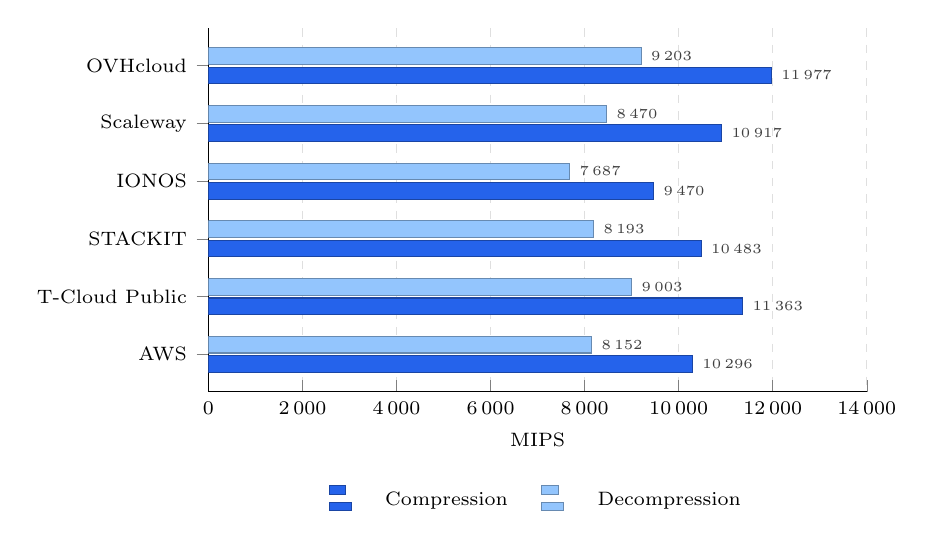
\begin{tikzpicture}
    \begin{axis}[benchh, xbar, /pgf/bar shift=0pt, height=6.2cm, xmin=0, xmax=14000,
      xlabel={MIPS},
      /pgf/bar width=6pt,
      legend style={font=\scriptsize, at={(0.5,-0.24)}, anchor=north,
                    legend columns=2, draw=none, column sep=1em},
      nodes near coords={\pgfmathprintnumber[fixed, precision=0, 1000 sep={\,}]{\pgfplotspointmeta}},
      point meta=x]
      \addplot[fill=bSerA, draw=bSerA!70!black, /pgf/bar shift=-3.5pt] coordinates {(11976.67,OVH) (10916.70,SCW) (9470.00,ION) (10483.30,STK) (11363.33,TCL) (10296.00,AWS)};
      \addplot[fill=bSerB, draw=bSerB!70!black, /pgf/bar shift=3.5pt] coordinates {(9203.33,OVH) (8470.00,SCW) (7686.70,ION) (8193.30,STK) (9003.33,TCL) (8151.70,AWS)};
      \legend{Compression, Decompression}
    \end{axis}
  \end{tikzpicture}
  \caption{Processor throughput across all cores, \texttt{pts/compress-7zip}.}
  \label{fig:bench-7zip}
\end{figure}

On a single core the six providers are close. \Cref{fig:bench-hint} shows that
the slowest, IONOS, completes 93 per cent of the operations of the fastest,
OVHcloud, and that \acs{AWS} is second by a margin of less than half of one per
cent. Once every core is working, as in \cref{fig:bench-7zip}, the spread widens:
OVHcloud compresses 26 per cent faster than IONOS, and \acs{AWS} falls to fifth of
the six, behind OVHcloud, T-Cloud Public, Scaleway and STACKIT. Decompression
places the providers in the same order. On a single core, then, the European
providers are close to \acs{AWS}: OVHcloud is slightly faster, and the others are
between 1 and 6 per cent slower. When all cores are used together, OVHcloud,
T-Cloud Public, Scaleway and STACKIT are all faster than \acs{AWS}, and IONOS
is the only European provider slower than it.

\subsubsection{Disk and application performance}
\label{sec:bench-disk}

\begin{figure}[htbp]
  \centering
  \begin{tikzpicture}
    \begin{axis}[benchh, xmin=0, xmax=10000, xlabel={transactions per second},nodes near coords={\pgfmathprintnumber[fixed, precision=0, 1000 sep={\,}]{\pgfplotspointmeta}},point meta=x]
      \addplot[fill=cProvB, draw=cProvB!70!black] coordinates {(8363.33,OVH)};
      \addplot[fill=cProvA, draw=cProvA!70!black] coordinates {(6513.00,SCW)};
      \addplot[fill=cProvD, draw=cProvD!70!black] coordinates {(5893.00,ION)};
      \addplot[fill=cProvE, draw=cProvE!70!black] coordinates {(6203.00,STK)};
      \addplot[fill=cProvC, draw=cProvC!70!black] coordinates {(6063.00,TCL)};
      \addplot[fill=cBase, draw=cBase!70!black] coordinates {(4470.00,AWS)};
    \end{axis}
  \end{tikzpicture}
  \caption{Disk transactions per second, \texttt{pts/postmark}.}
  \label{fig:bench-postmark}
\end{figure}

\begin{figure}[htbp]
  \centering
  \begin{tikzpicture}
    \begin{axis}[benchh, xmin=0, xmax=38000, xlabel={requests per second},nodes near coords={\pgfmathprintnumber[fixed, precision=0, 1000 sep={\,}]{\pgfplotspointmeta}},point meta=x]
      \addplot[fill=cProvB, draw=cProvB!70!black] coordinates {(32477.17,OVH)};
      \addplot[fill=cProvA, draw=cProvA!70!black] coordinates {(29423.80,SCW)};
      \addplot[fill=cProvD, draw=cProvD!70!black] coordinates {(27790.30,ION)};
      \addplot[fill=cProvE, draw=cProvE!70!black] coordinates {(28790.30,STK)};
      \addplot[fill=cProvC, draw=cProvC!70!black] coordinates {(31183.73,TCL)};
      \addplot[fill=cBase, draw=cBase!70!black] coordinates {(30126.90,AWS)};
    \end{axis}
  \end{tikzpicture}
  \caption{Web requests served per second, \texttt{pts/apache}.}
  \label{fig:bench-apache}
\end{figure}

The disk results show the effect of OVHcloud's local storage.
\Cref{fig:bench-postmark} places OVHcloud first by a wide margin, at 8\,363
transactions per second, 87 per cent more than \acs{AWS}. The five machines with
network storage lie between 4\,470 and 6\,513, and \acs{AWS}, whose storage is also
network-attached, is the slowest of the six. The web server results in
\cref{fig:bench-apache} are closer together: OVHcloud serves 32\,477 requests per
second and IONOS, the slowest, 27\,790, a spread of 17 per cent. T-Cloud Public is
second and \acs{AWS} third.

\subsubsection{Network bandwidth}

\begin{figure}[htbp]
  \centering
  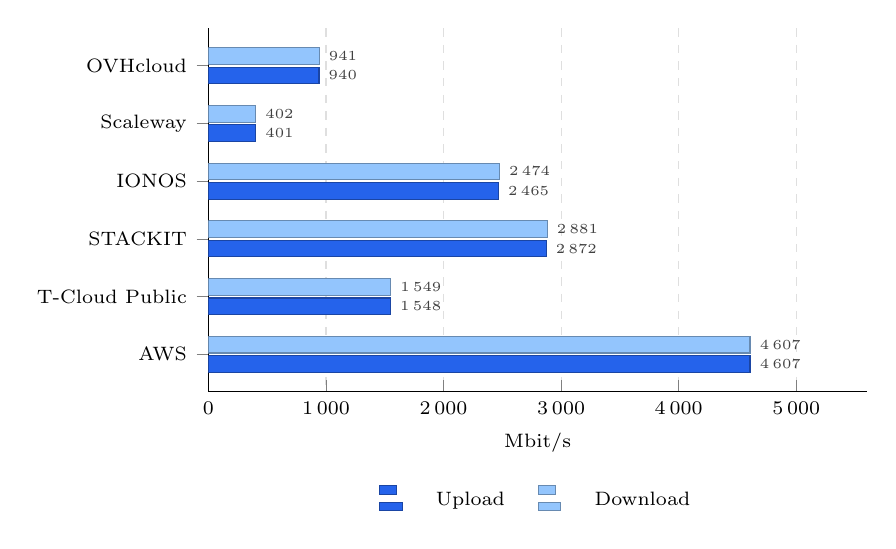
\begin{tikzpicture}
    \begin{axis}[benchh, xbar, /pgf/bar shift=0pt, height=6.2cm, xmin=0, xmax=5600,
      xlabel={Mbit/s}, /pgf/bar width=6pt,
      legend style={font=\scriptsize, at={(0.5,-0.24)}, anchor=north,
                    legend columns=2, draw=none, column sep=1em},
      nodes near coords={\pgfmathprintnumber[fixed, precision=0, 1000 sep={\,}]{\pgfplotspointmeta}},
      point meta=x]
      \addplot[fill=bSerA, draw=bSerA!70!black, /pgf/bar shift=-3.5pt] coordinates {(940.27,OVH) (400.99,SCW) (2465.30,ION) (2871.97,STK) (1548.00,TCL) (4607.00,AWS)};
      \addplot[fill=bSerB, draw=bSerB!70!black, /pgf/bar shift=3.5pt] coordinates {(941.20,OVH) (401.51,SCW) (2474.30,ION) (2880.97,STK) (1549.00,TCL) (4607.00,AWS)};
      \legend{Upload, Download}
    \end{axis}
  \end{tikzpicture}
  \caption{Network bandwidth between two machines in the same zone, \texttt{iperf3}.}
  \label{fig:bench-iperf}
\end{figure}

Network bandwidth separates the providers more than any other measurement.
\Cref{fig:bench-iperf} shows \acs{AWS} at 4\,607 Mbit/s, followed by STACKIT at 2\,872 and
IONOS at 2\,465; T-Cloud Public reaches 1\,548, OVHcloud 940, and Scaleway 401. The
bandwidth of \acs{AWS}, the fastest, is 11.5 times that of Scaleway, the slowest.
Upload and download are almost identical
for every provider.

Four of these results come from Cloud Mercato rather than from this study's own
measurements, and they were obtained differently. Cloud Mercato ran iperf3
between two machines in the same zone many times, varying the number of parallel
streams: 80 runs in each direction with one to four streams for \acs{AWS}, 50 with
one, two and four for T-Cloud Public, and 20 with two for Scaleway and StackIT
\cite{CloudMercato_AWS_m6i,CloudMercato_TSystems_s3,CloudMercato_Scaleway_POP2}.
The other two providers were measured in this study with three runs each. The
two sets are comparable in what they measure, but not in the number of runs
behind each figure.

The \acs{AWS} figure is the least stable of any in this study. The reported 80 runs range
from 758 to 11\,271 Mbit/s, and the spread does not follow the number of streams: with
one, two, three or four streams alike, results ran from about 760 to more than
9\,000 Mbit/s \cite{CloudMercato_AWS_m6i}. The average of 4\,607 Mbit/s therefore summarises a
result that varies by a factor of more than ten from one run to the next. The
Scaleway figure, by contrast, is stable and matches the product: Cloud Mercato
lists the network of this instance type at 381 Mbps, and the measured runs lie
between 390 and 462 \cite{CloudMercato_Scaleway_POP2}. The low figure for Scaleway
reflects the bandwidth the instance is sold with, not a fault in the
measurement.

\subsubsection{Provisioning time}

\begin{figure}[htbp]
  \centering
  \begin{tikzpicture}
    \begin{groupplot}[benchh,
      group style={group size=2 by 1, horizontal sep=0.6cm},
      width=0.5\textwidth, height=5.4cm, xmin=0,
      title style={font=\scriptsize\bfseries, yshift=-4pt},
      nodes near coords={\pgfmathprintnumber[fixed, precision=1, fixed zerofill]{\pgfplotspointmeta}}, point meta=x]
    \nextgroupplot[title={Boot time}, xmax=19, xlabel={seconds}]
      \addplot[fill=cProvB, draw=cProvB!70!black] coordinates {(10.63,OVH)};
      \addplot[fill=cProvA, draw=cProvA!70!black] coordinates {(14.10,SCW)};
      \addplot[fill=cProvD, draw=cProvD!70!black] coordinates {(15.27,ION)};
      \addplot[fill=cProvE, draw=cProvE!70!black] coordinates {(13.13,STK)};
      \addplot[fill=cProvC, draw=cProvC!70!black] coordinates {(15.80,TCL)};
      \addplot[fill=cBase, draw=cBase!70!black] coordinates {(13.30,AWS)};
    \nextgroupplot[title={Set-up time}, xmax=48, xlabel={seconds}, yticklabels={}]
      \addplot[fill=cProvB, draw=cProvB!70!black] coordinates {(22.27,OVH)};
      \addplot[fill=cProvA, draw=cProvA!70!black] coordinates {(34.43,SCW)};
      \addplot[fill=cProvD, draw=cProvD!70!black] coordinates {(28.80,ION)};
      \addplot[fill=cProvE, draw=cProvE!70!black] coordinates {(26.23,STK)};
      \addplot[fill=cProvC, draw=cProvC!70!black] coordinates {(39.80,TCL)};
      \addplot[fill=cBase, draw=cBase!70!black] coordinates {(23.40,AWS)};
    \end{groupplot}
  \end{tikzpicture}
  \caption{Time to boot until SSH is available, and to complete set-up, in seconds.}
  \label{fig:bench-bootsetup}
\end{figure}

\begin{figure}[htbp]
  \centering
  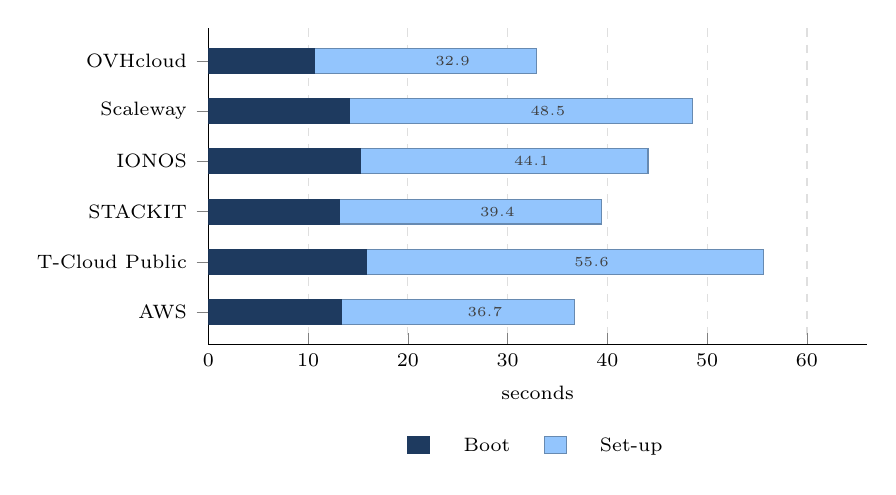
\begin{tikzpicture}
    \begin{axis}[benchh, xbar stacked, /pgf/bar shift=0pt, height=5.6cm, xmin=0, xmax=66,
      xlabel={seconds},
      legend style={font=\scriptsize, at={(0.5,-0.26)}, anchor=north,
                    legend columns=2, draw=none, column sep=1em}]
      \addplot[fill=bNavy, draw=bNavy] coordinates {(10.63,OVH) (14.10,SCW) (15.27,ION) (13.13,STK) (15.80,TCL) (13.30,AWS)};
      \addplot[fill=bSerB, draw=bSerB!70!black,
        nodes near coords={\pgfmathprintnumber[fixed, precision=1, fixed zerofill]{\pgfplotspointmeta}},
        point meta=explicit] coordinates {(22.27,OVH) [32.9] (34.43,SCW) [48.5] (28.80,ION) [44.1] (26.23,STK) [39.4] (39.80,TCL) [55.6] (23.40,AWS) [36.7]};
      \legend{Boot, Set-up}
    \end{axis}
  \end{tikzpicture}
  \caption{Total provisioning time, boot and set-up combined, in seconds.}
  \label{fig:bench-total}
\end{figure}

Every machine was ready for work in under a minute. OVHcloud boots fastest, in
10.63 seconds, and completes set-up fastest, in 22.27, so that it is ready in 32.9 seconds
in total (\cref{fig:bench-bootsetup,fig:bench-total}). \acs{AWS} follows at 36.7
seconds and STACKIT at 39.4. T-Cloud Public takes longest, at 55.6 seconds, most of
the difference arising in set-up rather than in boot. The scale of these times has
changed considerably since Gillam et al.\ took their measurements: they recorded
average boot times of around two minutes for \acs{AWS} machines
\cite{Gillam_FairBenchmarking_2013}, against between 10.63 and 15.8 seconds for every
provider here.

\subsection{Normalised comparison}
\label{sec:bench-composite}

Each test reports in its own unit, and the units cannot be added together. To
combine them, each result is expressed as a score out of 100 relative to the best
of the six providers on that test. For the six tests where a higher value is
better, the score is the provider's value divided by the best value; for boot and
set-up time, where a lower value is better, it is the best value divided by the
provider's. The composite score is the unweighted average of the eight:

\begin{equation}
  \label{eq:bench-score}
  s_{i} = 100 \times \frac{x_{i}}{\max_{j} x_{j}}
  \quad\text{or}\quad
  s_{i} = 100 \times \frac{\min_{j} x_{j}}{x_{i}},
  \qquad
  \text{composite} = \frac{1}{8}\sum_{m=1}^{8} s_{i,m}
\end{equation}

This follows Gillam et al.\ in setting each provider against the best result
achieved rather than against an external standard
\cite{Gillam_FairBenchmarking_2013}. \Cref{tab:bench-heatmap} gives every
measurement with its range, in the manner of their results tables, and colours
each cell by its score.

\begin{table}[htbp]
  \centering
  \caption{All eight measurements: the average, with the highest and lowest run
           beside it. Cell colour shows the score out of 100, and a box marks the
           best result in each column.}
  \label{tab:bench-heatmap}
  \scriptsize
  \setlength{\tabcolsep}{1.2pt}
  \renewcommand{\arraystretch}{1.5}
  \begin{tabular}{@{}>{\raggedright\arraybackslash}m{1.25cm} *{8}{>{\centering\arraybackslash}m{1.55cm}} >{\centering\arraybackslash}m{0.8cm}@{}}
    \toprule
    Provider & \shortstack{\textbf{Memory}\\[-1pt]{\tiny TRIAD}} & \shortstack{\textbf{CPU single}\\[-1pt]{\tiny hint}} & \shortstack{\textbf{CPU multi}\\[-1pt]{\tiny 7-zip}} & \shortstack{\textbf{Disk}\\[-1pt]{\tiny postmark}} & \shortstack{\textbf{Web}\\[-1pt]{\tiny apache}} & \shortstack{\textbf{Network}\\[-1pt]{\tiny iperf3}} & \shortstack{\textbf{Boot}\\[-1pt]{\tiny s, lower}} & \shortstack{\textbf{Set-up}\\[-1pt]{\tiny s, lower}} & \shortstack{\textbf{Comp.}\\[-1pt]{\tiny of 8}} \\
    \midrule
    AWS & \cellcolor[RGB]{187,247,208}\color[HTML]{14532D}{\setlength{\fboxsep}{1.2pt}\setlength{\fboxrule}{0.7pt}\color[RGB]{202,138,4}\fbox{\color[HTML]{14532D}\begin{tabular}{@{}r@{\hspace{2.5pt}}l@{}}{\fontsize{4.6}{5.3}\selectfont\color[HTML]{6D947D}\shortstack[r]{$\uparrow$21\,590\\$\downarrow$21\,351}} & \textbf{21\,477}\end{tabular}}} & \cellcolor[RGB]{187,247,208}\color[HTML]{14532D}\begin{tabular}{@{}r@{\hspace{2.5pt}}l@{}}{\fontsize{4.6}{5.3}\selectfont\color[HTML]{6D947D}\shortstack[r]{$\uparrow$445.9\\$\downarrow$441.3}} & 443.6\end{tabular} & \cellcolor[RGB]{206,248,196}\color[HTML]{14532D}\begin{tabular}{@{}r@{\hspace{2.5pt}}l@{}}{\fontsize{4.6}{5.3}\selectfont\color[HTML]{6D947D}\shortstack[r]{$\uparrow$10\,319\\$\downarrow$10\,275}} & 10\,296\end{tabular} & \cellcolor[RGB]{250,252,169}\color[HTML]{713F12}\begin{tabular}{@{}r@{\hspace{2.5pt}}l@{}}{\fontsize{4.6}{5.3}\selectfont\color[HTML]{A7886C}\shortstack[r]{$\uparrow$4\,510\\$\downarrow$4\,420}} & 4\,470\end{tabular} & \cellcolor[RGB]{196,248,202}\color[HTML]{14532D}\begin{tabular}{@{}r@{\hspace{2.5pt}}l@{}}{\fontsize{4.6}{5.3}\selectfont\color[HTML]{6D947D}\shortstack[r]{$\uparrow$30\,421\\$\downarrow$29\,850}} & 30\,127\end{tabular} & \cellcolor[RGB]{187,247,208}\color[HTML]{14532D}{\setlength{\fboxsep}{1.2pt}\setlength{\fboxrule}{0.7pt}\color[RGB]{202,138,4}\fbox{\color[HTML]{14532D}\begin{tabular}{@{}r@{\hspace{2.5pt}}l@{}}{\fontsize{4.6}{5.3}\selectfont\color[HTML]{6D947D}\shortstack[r]{$\uparrow$11\,271\\$\downarrow$758}} & \textbf{4\,607}\end{tabular}}} & \cellcolor[RGB]{214,249,191}\color[HTML]{14532D}\begin{tabular}{@{}r@{\hspace{2.5pt}}l@{}}{\fontsize{4.6}{5.3}\selectfont\color[HTML]{6D947D}\shortstack[r]{$\uparrow$13.8\\$\downarrow$12.9}} & 13.3\end{tabular} & \cellcolor[RGB]{194,248,204}\color[HTML]{14532D}\begin{tabular}{@{}r@{\hspace{2.5pt}}l@{}}{\fontsize{4.6}{5.3}\selectfont\color[HTML]{6D947D}\shortstack[r]{$\uparrow$24.8\\$\downarrow$22.1}} & 23.4\end{tabular} & \cellcolor[RGB]{203,248,198}\color[HTML]{14532D}\textbf{88.4} \\
    OVHcloud & \cellcolor[RGB]{215,249,190}\color[HTML]{14532D}\begin{tabular}{@{}r@{\hspace{2.5pt}}l@{}}{\fontsize{4.6}{5.3}\selectfont\color[HTML]{6D947D}\shortstack[r]{$\uparrow$16\,988\\$\downarrow$16\,900}} & 16\,944\end{tabular} & \cellcolor[RGB]{187,247,208}\color[HTML]{14532D}{\setlength{\fboxsep}{1.2pt}\setlength{\fboxrule}{0.7pt}\color[RGB]{202,138,4}\fbox{\color[HTML]{14532D}\begin{tabular}{@{}r@{\hspace{2.5pt}}l@{}}{\fontsize{4.6}{5.3}\selectfont\color[HTML]{6D947D}\shortstack[r]{$\uparrow$448.5\\$\downarrow$442.1}} & \textbf{445.3}\end{tabular}}} & \cellcolor[RGB]{187,247,208}\color[HTML]{14532D}{\setlength{\fboxsep}{1.2pt}\setlength{\fboxrule}{0.7pt}\color[RGB]{202,138,4}\fbox{\color[HTML]{14532D}\begin{tabular}{@{}r@{\hspace{2.5pt}}l@{}}{\fontsize{4.6}{5.3}\selectfont\color[HTML]{6D947D}\shortstack[r]{$\uparrow$12\,100\\$\downarrow$11\,850}} & \textbf{11\,977}\end{tabular}}} & \cellcolor[RGB]{187,247,208}\color[HTML]{14532D}{\setlength{\fboxsep}{1.2pt}\setlength{\fboxrule}{0.7pt}\color[RGB]{202,138,4}\fbox{\color[HTML]{14532D}\begin{tabular}{@{}r@{\hspace{2.5pt}}l@{}}{\fontsize{4.6}{5.3}\selectfont\color[HTML]{6D947D}\shortstack[r]{$\uparrow$8\,480\\$\downarrow$8\,250}} & \textbf{8\,363}\end{tabular}}} & \cellcolor[RGB]{187,247,208}\color[HTML]{14532D}{\setlength{\fboxsep}{1.2pt}\setlength{\fboxrule}{0.7pt}\color[RGB]{202,138,4}\fbox{\color[HTML]{14532D}\begin{tabular}{@{}r@{\hspace{2.5pt}}l@{}}{\fontsize{4.6}{5.3}\selectfont\color[HTML]{6D947D}\shortstack[r]{$\uparrow$32\,850\\$\downarrow$32\,101}} & \textbf{32\,477}\end{tabular}}} & \cellcolor[RGB]{254,222,188}\color[HTML]{7F1D1D}\begin{tabular}{@{}r@{\hspace{2.5pt}}l@{}}{\fontsize{4.6}{5.3}\selectfont\color[HTML]{B07373}\shortstack[r]{$\uparrow$943\\$\downarrow$938}} & 940\end{tabular} & \cellcolor[RGB]{187,247,208}\color[HTML]{14532D}{\setlength{\fboxsep}{1.2pt}\setlength{\fboxrule}{0.7pt}\color[RGB]{202,138,4}\fbox{\color[HTML]{14532D}\begin{tabular}{@{}r@{\hspace{2.5pt}}l@{}}{\fontsize{4.6}{5.3}\selectfont\color[HTML]{6D947D}\shortstack[r]{$\uparrow$11.1\\$\downarrow$10.2}} & \textbf{10.63}\end{tabular}}} & \cellcolor[RGB]{187,247,208}\color[HTML]{14532D}{\setlength{\fboxsep}{1.2pt}\setlength{\fboxrule}{0.7pt}\color[RGB]{202,138,4}\fbox{\color[HTML]{14532D}\begin{tabular}{@{}r@{\hspace{2.5pt}}l@{}}{\fontsize{4.6}{5.3}\selectfont\color[HTML]{6D947D}\shortstack[r]{$\uparrow$23.2\\$\downarrow$21.5}} & \textbf{22.27}\end{tabular}}} & \cellcolor[RGB]{204,248,197}\color[HTML]{14532D}\textbf{87.4} \\
    STACKIT & \cellcolor[RGB]{203,248,198}\color[HTML]{14532D}\begin{tabular}{@{}r@{\hspace{2.5pt}}l@{}}{\fontsize{4.6}{5.3}\selectfont\color[HTML]{6D947D}\shortstack[r]{$\uparrow$19\,110\\$\downarrow$18\,851}} & 18\,994\end{tabular} & \cellcolor[RGB]{194,248,204}\color[HTML]{14532D}\begin{tabular}{@{}r@{\hspace{2.5pt}}l@{}}{\fontsize{4.6}{5.3}\selectfont\color[HTML]{6D947D}\shortstack[r]{$\uparrow$426.8\\$\downarrow$421.4}} & 424.3\end{tabular} & \cellcolor[RGB]{203,248,198}\color[HTML]{14532D}\begin{tabular}{@{}r@{\hspace{2.5pt}}l@{}}{\fontsize{4.6}{5.3}\selectfont\color[HTML]{6D947D}\shortstack[r]{$\uparrow$10\,550\\$\downarrow$10\,420}} & 10\,483\end{tabular} & \cellcolor[RGB]{222,250,186}\color[HTML]{713F12}\begin{tabular}{@{}r@{\hspace{2.5pt}}l@{}}{\fontsize{4.6}{5.3}\selectfont\color[HTML]{A7886C}\shortstack[r]{$\uparrow$6\,280\\$\downarrow$6\,120}} & 6\,203\end{tabular} & \cellcolor[RGB]{202,248,199}\color[HTML]{14532D}\begin{tabular}{@{}r@{\hspace{2.5pt}}l@{}}{\fontsize{4.6}{5.3}\selectfont\color[HTML]{6D947D}\shortstack[r]{$\uparrow$29\,100\\$\downarrow$28\,451}} & 28\,790\end{tabular} & \cellcolor[RGB]{238,251,176}\color[HTML]{713F12}\begin{tabular}{@{}r@{\hspace{2.5pt}}l@{}}{\fontsize{4.6}{5.3}\selectfont\color[HTML]{A7886C}\shortstack[r]{$\uparrow$2\,891\\$\downarrow$2\,850}} & 2\,872\end{tabular} & \cellcolor[RGB]{212,249,192}\color[HTML]{14532D}\begin{tabular}{@{}r@{\hspace{2.5pt}}l@{}}{\fontsize{4.6}{5.3}\selectfont\color[HTML]{6D947D}\shortstack[r]{$\uparrow$13.5\\$\downarrow$12.8}} & 13.13\end{tabular} & \cellcolor[RGB]{207,249,195}\color[HTML]{14532D}\begin{tabular}{@{}r@{\hspace{2.5pt}}l@{}}{\fontsize{4.6}{5.3}\selectfont\color[HTML]{6D947D}\shortstack[r]{$\uparrow$27.1\\$\downarrow$25.4}} & 26.23\end{tabular} & \cellcolor[RGB]{210,249,194}\color[HTML]{14532D}\textbf{82.8} \\
    IONOS & \cellcolor[RGB]{194,248,204}\color[HTML]{14532D}\begin{tabular}{@{}r@{\hspace{2.5pt}}l@{}}{\fontsize{4.6}{5.3}\selectfont\color[HTML]{6D947D}\shortstack[r]{$\uparrow$20\,510\\$\downarrow$20\,251}} & 20\,394\end{tabular} & \cellcolor[RGB]{196,248,202}\color[HTML]{14532D}\begin{tabular}{@{}r@{\hspace{2.5pt}}l@{}}{\fontsize{4.6}{5.3}\selectfont\color[HTML]{6D947D}\shortstack[r]{$\uparrow$418.9\\$\downarrow$412.4}} & 415.6\end{tabular} & \cellcolor[RGB]{215,249,190}\color[HTML]{14532D}\begin{tabular}{@{}r@{\hspace{2.5pt}}l@{}}{\fontsize{4.6}{5.3}\selectfont\color[HTML]{6D947D}\shortstack[r]{$\uparrow$9\,510\\$\downarrow$9\,420}} & 9\,470\end{tabular} & \cellcolor[RGB]{227,250,183}\color[HTML]{713F12}\begin{tabular}{@{}r@{\hspace{2.5pt}}l@{}}{\fontsize{4.6}{5.3}\selectfont\color[HTML]{A7886C}\shortstack[r]{$\uparrow$5\,950\\$\downarrow$5\,820}} & 5\,893\end{tabular} & \cellcolor[RGB]{206,248,196}\color[HTML]{14532D}\begin{tabular}{@{}r@{\hspace{2.5pt}}l@{}}{\fontsize{4.6}{5.3}\selectfont\color[HTML]{6D947D}\shortstack[r]{$\uparrow$28\,100\\$\downarrow$27\,451}} & 27\,790\end{tabular} & \cellcolor[RGB]{249,252,169}\color[HTML]{713F12}\begin{tabular}{@{}r@{\hspace{2.5pt}}l@{}}{\fontsize{4.6}{5.3}\selectfont\color[HTML]{A7886C}\shortstack[r]{$\uparrow$2\,481\\$\downarrow$2\,450}} & 2\,465\end{tabular} & \cellcolor[RGB]{227,250,183}\color[HTML]{713F12}\begin{tabular}{@{}r@{\hspace{2.5pt}}l@{}}{\fontsize{4.6}{5.3}\selectfont\color[HTML]{A7886C}\shortstack[r]{$\uparrow$15.8\\$\downarrow$14.9}} & 15.27\end{tabular} & \cellcolor[RGB]{218,249,189}\color[HTML]{14532D}\begin{tabular}{@{}r@{\hspace{2.5pt}}l@{}}{\fontsize{4.6}{5.3}\selectfont\color[HTML]{6D947D}\shortstack[r]{$\uparrow$30.1\\$\downarrow$27.9}} & 28.8\end{tabular} & \cellcolor[RGB]{216,249,190}\color[HTML]{14532D}\textbf{78.0} \\
    \shortstack[l]{T-Cloud\\Public} & \cellcolor[RGB]{195,248,203}\color[HTML]{14532D}\begin{tabular}{@{}r@{\hspace{2.5pt}}l@{}}{\fontsize{4.6}{5.3}\selectfont\color[HTML]{6D947D}\shortstack[r]{$\uparrow$20\,250\\$\downarrow$19\,951}} & 20\,100\end{tabular} & \cellcolor[RGB]{195,248,203}\color[HTML]{14532D}\begin{tabular}{@{}r@{\hspace{2.5pt}}l@{}}{\fontsize{4.6}{5.3}\selectfont\color[HTML]{6D947D}\shortstack[r]{$\uparrow$421.8\\$\downarrow$415.2}} & 418.5\end{tabular} & \cellcolor[RGB]{194,248,204}\color[HTML]{14532D}\begin{tabular}{@{}r@{\hspace{2.5pt}}l@{}}{\fontsize{4.6}{5.3}\selectfont\color[HTML]{6D947D}\shortstack[r]{$\uparrow$11\,480\\$\downarrow$11\,250}} & 11\,363\end{tabular} & \cellcolor[RGB]{225,250,184}\color[HTML]{713F12}\begin{tabular}{@{}r@{\hspace{2.5pt}}l@{}}{\fontsize{4.6}{5.3}\selectfont\color[HTML]{A7886C}\shortstack[r]{$\uparrow$6\,150\\$\downarrow$5\,980}} & 6\,063\end{tabular} & \cellcolor[RGB]{192,247,205}\color[HTML]{14532D}\begin{tabular}{@{}r@{\hspace{2.5pt}}l@{}}{\fontsize{4.6}{5.3}\selectfont\color[HTML]{6D947D}\shortstack[r]{$\uparrow$31\,521\\$\downarrow$30\,850}} & 31\,184\end{tabular} & \cellcolor[RGB]{254,236,178}\color[HTML]{7F1D1D}\begin{tabular}{@{}r@{\hspace{2.5pt}}l@{}}{\fontsize{4.6}{5.3}\selectfont\color[HTML]{B07373}\shortstack[r]{$\uparrow$1\,578\\$\downarrow$1\,538}} & 1\,548\end{tabular} & \cellcolor[RGB]{231,250,180}\color[HTML]{713F12}\begin{tabular}{@{}r@{\hspace{2.5pt}}l@{}}{\fontsize{4.6}{5.3}\selectfont\color[HTML]{A7886C}\shortstack[r]{$\uparrow$16.4\\$\downarrow$15.2}} & 15.8\end{tabular} & \cellcolor[RGB]{246,251,171}\color[HTML]{713F12}\begin{tabular}{@{}r@{\hspace{2.5pt}}l@{}}{\fontsize{4.6}{5.3}\selectfont\color[HTML]{A7886C}\shortstack[r]{$\uparrow$41.2\\$\downarrow$38.5}} & 39.8\end{tabular} & \cellcolor[RGB]{219,249,188}\color[HTML]{14532D}\textbf{76.0} \\
    Scaleway & \cellcolor[RGB]{200,248,200}\color[HTML]{14532D}\begin{tabular}{@{}r@{\hspace{2.5pt}}l@{}}{\fontsize{4.6}{5.3}\selectfont\color[HTML]{6D947D}\shortstack[r]{$\uparrow$19\,490\\$\downarrow$19\,281}} & 19\,384\end{tabular} & \cellcolor[RGB]{190,247,206}\color[HTML]{14532D}\begin{tabular}{@{}r@{\hspace{2.5pt}}l@{}}{\fontsize{4.6}{5.3}\selectfont\color[HTML]{6D947D}\shortstack[r]{$\uparrow$439.9\\$\downarrow$435.1}} & 437.5\end{tabular} & \cellcolor[RGB]{199,248,200}\color[HTML]{14532D}\begin{tabular}{@{}r@{\hspace{2.5pt}}l@{}}{\fontsize{4.6}{5.3}\selectfont\color[HTML]{6D947D}\shortstack[r]{$\uparrow$10\,980\\$\downarrow$10\,850}} & 10\,917\end{tabular} & \cellcolor[RGB]{216,249,190}\color[HTML]{14532D}\begin{tabular}{@{}r@{\hspace{2.5pt}}l@{}}{\fontsize{4.6}{5.3}\selectfont\color[HTML]{6D947D}\shortstack[r]{$\uparrow$6\,580\\$\downarrow$6\,450}} & 6\,513\end{tabular} & \cellcolor[RGB]{199,248,200}\color[HTML]{14532D}\begin{tabular}{@{}r@{\hspace{2.5pt}}l@{}}{\fontsize{4.6}{5.3}\selectfont\color[HTML]{6D947D}\shortstack[r]{$\uparrow$29\,751\\$\downarrow$29\,100}} & 29\,424\end{tabular} & \cellcolor[RGB]{254,211,196}\color[HTML]{7F1D1D}\begin{tabular}{@{}r@{\hspace{2.5pt}}l@{}}{\fontsize{4.6}{5.3}\selectfont\color[HTML]{B07373}\shortstack[r]{$\uparrow$462\\$\downarrow$390}} & 401\end{tabular} & \cellcolor[RGB]{221,250,187}\color[HTML]{14532D}\begin{tabular}{@{}r@{\hspace{2.5pt}}l@{}}{\fontsize{4.6}{5.3}\selectfont\color[HTML]{6D947D}\shortstack[r]{$\uparrow$14.5\\$\downarrow$13.8}} & 14.1\end{tabular} & \cellcolor[RGB]{234,250,179}\color[HTML]{713F12}\begin{tabular}{@{}r@{\hspace{2.5pt}}l@{}}{\fontsize{4.6}{5.3}\selectfont\color[HTML]{A7886C}\shortstack[r]{$\uparrow$36.1\\$\downarrow$33.2}} & 34.43\end{tabular} & \cellcolor[RGB]{221,250,187}\color[HTML]{713F12}\textbf{74.6} \\
    \bottomrule
  \end{tabular}

  \vspace{4pt}
  {\scriptsize\raggedright Low \tikz\fill[fill={rgb,255:red,254;green,202;blue,202}] (0,0) rectangle (0.42,0.24); \tikz\fill[fill={rgb,255:red,254;green,222;blue,188}] (0,0) rectangle (0.42,0.24); \tikz\fill[fill={rgb,255:red,254;green,242;blue,173}] (0,0) rectangle (0.42,0.24); \tikz\fill[fill={rgb,255:red,241;green,251;blue,174}] (0,0) rectangle (0.42,0.24); \tikz\fill[fill={rgb,255:red,214;green,249;blue,191}] (0,0) rectangle (0.42,0.24); \tikz\fill[fill={rgb,255:red,187;green,247;blue,208}] (0,0) rectangle (0.42,0.24); High \quad Memory in MB/s, CPU single in million
  MIPS, CPU multi in MIPS, disk in transactions and web in requests per second,
  network in Mbit/s. Every value is the average of three runs, except network bandwidth for AWS (80), T-Cloud Public (50), Scaleway (20), which are Cloud Mercato's.\par}
\end{table}

\begin{figure}[htbp]
  \centering
  \begin{tikzpicture}
    \begin{axis}[benchh, xmin=0, xmax=105, xlabel={score out of 100},nodes near coords={\pgfmathprintnumber[fixed, precision=1, fixed zerofill]{\pgfplotspointmeta}},point meta=x]
      \addplot[fill=cProvB, draw=cProvB!70!black] coordinates {(87.4,OVH)};
      \addplot[fill=cProvA, draw=cProvA!70!black] coordinates {(74.6,SCW)};
      \addplot[fill=cProvD, draw=cProvD!70!black] coordinates {(78.0,ION)};
      \addplot[fill=cProvE, draw=cProvE!70!black] coordinates {(82.8,STK)};
      \addplot[fill=cProvC, draw=cProvC!70!black] coordinates {(76.0,TCL)};
      \addplot[fill=cBase, draw=cBase!70!black] coordinates {(88.4,AWS)};
    \end{axis}
  \end{tikzpicture}
  \caption{Composite performance score, the average of the eight normalised measurements.}
  \label{fig:bench-composite}
\end{figure}

The composite scores lie within 13.8 points of each other (\cref{fig:bench-composite}).
\acs{AWS} ranks first at 88.4, followed closely by OVHcloud at 87.4, then STACKIT
at 82.8, IONOS at 78.0, T-Cloud Public at 76.0 and Scaleway at 74.6. The ranking
at the top rests on a single measurement. OVHcloud records the best result on
six of the eight tests --- single-core and multi-core processing, disk, web
serving, boot and set-up --- and \acs{AWS} on the other two, memory and network.
On network bandwidth \acs{AWS} scores 100 while no European provider scores more
than 62, and that one column accounts for its lead: without it, OVHcloud's average
across the remaining seven tests would be 97.0 and that of \acs{AWS} 86.7.


\subsection{Price and value for money}

\begin{figure}[htbp]
  \centering
  \begin{tikzpicture}
    \begin{axis}[benchh, xmin=0, xmax=0.135, xlabel={euros per hour},nodes near coords={\texteuro\pgfmathprintnumber[fixed, precision=3, fixed zerofill]{\pgfplotspointmeta}},point meta=x, xtick={0,0.03,0.06,0.09,0.12}, xticklabel style={/pgf/number format/fixed, /pgf/number format/precision=2}]
      \addplot[fill=cProvB, draw=cProvB!70!black] coordinates {(0.060,OVH)};
      \addplot[fill=cProvA, draw=cProvA!70!black] coordinates {(0.074,SCW)};
      \addplot[fill=cProvD, draw=cProvD!70!black] coordinates {(0.041,ION)};
      \addplot[fill=cProvE, draw=cProvE!70!black] coordinates {(0.098,STK)};
      \addplot[fill=cProvC, draw=cProvC!70!black] coordinates {(0.114,TCL)};
      \addplot[fill=cBase, draw=cBase!70!black] coordinates {(0.106,AWS)};
    \end{axis}
  \end{tikzpicture}
  \caption{Hourly list price, 2\,vCPU and 8\,GB of memory.}
  \label{fig:bench-price}
\end{figure}

\begin{figure}[htbp]
  \centering
  \begin{tikzpicture}
    \begin{axis}[benchh, height=5.4cm, xmin=0, xmax=2250, xlabel={composite score per euro per hour},
      symbolic y coords={V0,V1,V2,V3,V4,V5}, ytick={V0,V1,V2,V3,V4,V5},
      yticklabels={IONOS,OVHcloud,Scaleway,STACKIT,AWS,{T-Cloud Public}},
      nodes near coords={\pgfmathprintnumber[fixed, precision=0, 1000 sep={\,}]{\pgfplotspointmeta}},
      point meta=x]
      \addplot[fill=cProvD, draw=cProvD!70!black] coordinates {(1902,V0)};
      \addplot[fill=cProvB, draw=cProvB!70!black] coordinates {(1457,V1)};
      \addplot[fill=cProvA, draw=cProvA!70!black] coordinates {(1008,V2)};
      \addplot[fill=cProvE, draw=cProvE!70!black] coordinates {(845,V3)};
      \addplot[fill=cBase, draw=cBase!70!black] coordinates {(834,V4)};
      \addplot[fill=cProvC, draw=cProvC!70!black] coordinates {(667,V5)};
    \end{axis}
  \end{tikzpicture}
  \caption{Composite score per euro per hour, ordered from the best value.}
  \label{fig:bench-value}
\end{figure}

\begin{figure}[htbp]
  \centering
  \begin{tikzpicture}
    \begin{groupplot}[benchh,
      group style={group size=2 by 3, horizontal sep=0.6cm, vertical sep=1.2cm},
      width=0.5\textwidth, height=4.6cm, xmin=0, xmax=2800,
      xtick={0,1000,2000}, xticklabels={0,1k,2k}, /pgf/bar width=6pt,
      title style={font=\scriptsize\bfseries, yshift=-4pt},
      nodes near coords={\pgfmathprintnumber[fixed, precision=0, 1000 sep={\,}]{\pgfplotspointmeta}},
      nodes near coords style={font=\tiny, anchor=west, black!75},
      point meta=x]
    \nextgroupplot[title={Memory / \texteuro}]
      \addplot[fill=cProvB, draw=cProvB!70!black] coordinates {(1317,OVH)};
      \addplot[fill=cProvA, draw=cProvA!70!black] coordinates {(1216,SCW)};
      \addplot[fill=cProvD, draw=cProvD!70!black] coordinates {(2317,ION)};
      \addplot[fill=cProvE, draw=cProvE!70!black] coordinates {(898,STK)};
      \addplot[fill=cProvC, draw=cProvC!70!black] coordinates {(825,TCL)};
      \addplot[fill=cBase, draw=cBase!70!black] coordinates {(943,AWS)};
    \nextgroupplot[title={CPU single / \texteuro}, yticklabels={}]
      \addplot[fill=cProvB, draw=cProvB!70!black] coordinates {(1667,OVH)};
      \addplot[fill=cProvA, draw=cProvA!70!black] coordinates {(1324,SCW)};
      \addplot[fill=cProvD, draw=cProvD!70!black] coordinates {(2268,ION)};
      \addplot[fill=cProvE, draw=cProvE!70!black] coordinates {(969,STK)};
      \addplot[fill=cProvC, draw=cProvC!70!black] coordinates {(825,TCL)};
      \addplot[fill=cBase, draw=cBase!70!black] coordinates {(943,AWS)};
    \nextgroupplot[title={CPU multi / \texteuro}]
      \addplot[fill=cProvB, draw=cProvB!70!black] coordinates {(1667,OVH)};
      \addplot[fill=cProvA, draw=cProvA!70!black] coordinates {(1230,SCW)};
      \addplot[fill=cProvD, draw=cProvD!70!black] coordinates {(1927,ION)};
      \addplot[fill=cProvE, draw=cProvE!70!black] coordinates {(898,STK)};
      \addplot[fill=cProvC, draw=cProvC!70!black] coordinates {(833,TCL)};
      \addplot[fill=cBase, draw=cBase!70!black] coordinates {(811,AWS)};
    \nextgroupplot[title={Disk / \texteuro}, yticklabels={}]
      \addplot[fill=cProvB, draw=cProvB!70!black] coordinates {(1667,OVH)};
      \addplot[fill=cProvA, draw=cProvA!70!black] coordinates {(1054,SCW)};
      \addplot[fill=cProvD, draw=cProvD!70!black] coordinates {(1707,ION)};
      \addplot[fill=cProvE, draw=cProvE!70!black] coordinates {(755,STK)};
      \addplot[fill=cProvC, draw=cProvC!70!black] coordinates {(632,TCL)};
      \addplot[fill=cBase, draw=cBase!70!black] coordinates {(500,AWS)};
    \nextgroupplot[title={Web / \texteuro}]
      \addplot[fill=cProvB, draw=cProvB!70!black] coordinates {(1667,OVH)};
      \addplot[fill=cProvA, draw=cProvA!70!black] coordinates {(1230,SCW)};
      \addplot[fill=cProvD, draw=cProvD!70!black] coordinates {(2098,ION)};
      \addplot[fill=cProvE, draw=cProvE!70!black] coordinates {(908,STK)};
      \addplot[fill=cProvC, draw=cProvC!70!black] coordinates {(842,TCL)};
      \addplot[fill=cBase, draw=cBase!70!black] coordinates {(877,AWS)};
    \nextgroupplot[title={Network / \texteuro}, yticklabels={}]
      \addplot[fill=cProvB, draw=cProvB!70!black] coordinates {(333,OVH)};
      \addplot[fill=cProvA, draw=cProvA!70!black] coordinates {(122,SCW)};
      \addplot[fill=cProvD, draw=cProvD!70!black] coordinates {(1317,ION)};
      \addplot[fill=cProvE, draw=cProvE!70!black] coordinates {(633,STK)};
      \addplot[fill=cProvC, draw=cProvC!70!black] coordinates {(298,TCL)};
      \addplot[fill=cBase, draw=cBase!70!black] coordinates {(943,AWS)};
    \end{groupplot}
  \end{tikzpicture}
  \caption{Score per euro per hour for each measurement.}
  \label{fig:bench-value-metric}
\end{figure}

The hourly list prices recorded at the time of testing range from \texteuro0.041 for IONOS
to \texteuro0.114 for T-Cloud Public (\cref{fig:bench-price}). \acs{AWS}, at \texteuro0.106, is the second
most expensive of the six. Dividing the composite score by the hourly price gives
the performance obtained for each euro, shown in \cref{fig:bench-value}. On this
measure the order changes almost completely. IONOS delivers the most performance
per euro, 2.3 times as much as \acs{AWS}, because it has the lowest price and a
composite only 10.4 points below the leader; OVHcloud is second at 1.7 times
\acs{AWS}. T-Cloud Public, with the highest price, delivers the least.
\Cref{fig:bench-value-metric} shows the same calculation for each measurement
separately: IONOS delivers the most per euro on every one of the six, including
network bandwidth, the one measurement on which \acs{AWS} leads outright.


\subsection{Findings and scope}
\label{sec:bench-findings}

On a machine of the same size, the European providers are not behind the
baseline. OVHcloud matches or exceeds \acs{AWS} on six of the eight measurements at
57 per cent of its hourly price, and four European providers --- OVHcloud,
T-Cloud Public, Scaleway and STACKIT --- outperform it when all processor cores
are in use.
The capability gap measured in \cref{sec:method-study2} and the financial gap
measured in \cref{sec:method-study3} concern the breadth of what a provider
offers and the resources behind it; neither reappears in the performance of an
individual machine. The one clear advantage of \acs{AWS} is network bandwidth
between machines, which matters most to applications spread across many of them.
Measured per euro, IONOS and OVHcloud offer the most performance of the six, and
the highest-priced provider, T-Cloud Public, the least.

These results describe one size of machine, in one region per provider, measured
on a single day. Measured against the principles of Papadopoulos et al., the study
describes its set-up, states its units, reports each result with its range and
includes cost, but it falls short on two of them
\cite{Papadopoulos_Principles_2021}. Each of the author's measurements rests on
three runs, whereas Gillam et al.\ typically ran ten for each machine type and
found that machines of the same specification from the same provider can differ
substantially in performance \cite{Gillam_FairBenchmarking_2013}; and with three
runs, no statistical test of the differences between providers was possible. The
research reviewed above also shows that variation differs between providers and
that providers change their infrastructure over time
\cite{LeitnerCito_Chaos_2016}. The comparison therefore establishes that European
performance is competitive at this size and price on the date it was measured; it
does not establish how consistently a newly provisioned machine will deliver it,
or whether the ranking will hold as the providers renew their hardware.


\section{Limitations of these Research Studies}
\label{sec:design-limitations}

Every study in this chapter had to work with what could be found, read or
measured from the outside. That brought limits of its own, and some of them were
a real struggle throughout the research. They are set out here so that the
results that follow can be read with them in mind.

\subsection*{Relying on what the providers publish}

The sovereignty and capability studies could only be as good as the documents
behind them. Most providers do not set out in one place who owns them, which laws
apply to them, or exactly which services they offer. That information had to be
pieced together from websites, product pages, certificates and company filings,
often written for marketing rather than for checking. Where a provider published
little, there was little to assess, and its score suffered for it. A low score in
these studies can therefore mean that a provider explains itself poorly, not
necessarily that it protects data poorly. It also means that the studies record
what providers say about themselves. Whether they behave that way in practice
could not be tested from the outside.

\subsection*{Missing financial figures}

The financial study met the same problem in a sharper form. Several of the cloud
businesses studied belong to much larger groups, and those groups report their
results as a whole. They do not say how much their cloud business earns on its
own. For T-Cloud Public, STACKIT and Scaleway, the nearest published figure had
to stand in for the cloud business, and for Scaleway the last such figure is from
2022 (\cref{tab:study3-growth}). Comparisons with \acs{AWS} for these providers can
therefore only be given as a range, not as a single number. The investment
announcements raised a similar difficulty. A company can announce that it will
invest a sum by a given year, but whether that money is actually spent cannot be
seen from outside. The study could only record what was promised and by when.

\subsection*{A single moment in time}

Cloud providers change quickly. During this research alone, Deutsche Telekom
renamed its public cloud \cite{TCloudPublic_2026}. Every result in this chapter describes the providers as they were when the data
was collected. A provider that scored poorly may since have closed some of its
gaps, and the opposite is also possible. The figures are a snapshot, not a
permanent verdict, which is one reason CloudSov was built so that the assessments
can be repeated.

\subsection*{Measuring against \acs{AWS}}

The capability study measures each European provider against the services that
\acs{AWS} offers. This makes the comparison clear, because it asks how much of
what an enterprise already uses could be replaced. It also has a cost. A provider
that offers something \acs{AWS} does not receive no credit for it, so the study
shows how close each provider comes to \acs{AWS}, not everything each provider is
good at.

\subsection*{The needs of one company}

The requirements behind the capability study come from one enterprise, Alps
Alpine, and its current systems. Another company, with different systems or in a
different industry, would need a different set of services and could reach a
different conclusion about the same providers. The method can be applied to any
company, but the results in this chapter answer the question for this one.

\subsection*{Limits of the performance tests}

The performance tests were the only part of the research that could be measured
directly, and even they had limits. Each provider was tested with one comparable
machine, in one location, and the tests were run over a short period rather than
weeks or months. Each test was repeated three times, which shows roughly how
steady a result is but is too few to prove that small differences between
providers are real (\cref{sec:bench-findings}). For three
network results, figures published by Cloud Mercato were used instead, and these
rest on a different number of runs from the rest.

\subsection*{What was not assessed}

Finally, some things that matter a great deal to a customer lay outside what this
research could measure. How quickly a provider responds when something goes
wrong, how often its services fail, how good its support is, and how easy it is
to leave all depend on experience over time, from inside a working relationship.
None of these could be assessed fairly from published material or from a short
test, so none of them is included in the results.
